\documentclass[11pt,a4paper]{article}
\usepackage[utf8]{inputenc}
\usepackage[T1]{fontenc}
\usepackage[english]{babel}
\usepackage[english]{isodate}
\usepackage[paper=a4paper]{geometry}
\newgeometry{top=3.5cm,bottom=2.5cm,right=2.5cm,left=2.5cm}
\usepackage{graphicx}
\usepackage{comment}
\usepackage{fancyhdr}
\usepackage{framed}
\usepackage{lastpage}
\usepackage[hidelinks]{hyperref}
\usepackage{tabularx}
\usepackage[table]{xcolor}
\usepackage{enumitem}
\usepackage{mdwlist}
\usepackage{placeins}
\usepackage{amsmath}
\usepackage{xcolor}
\usepackage{listings}
\usepackage{amssymb}
\usepackage{amsthm}
\usepackage{xparse}
\usepackage{float}
\usepackage{chngcntr}

\counterwithin*{equation}{section}
\counterwithin*{equation}{subsection}


\begin{document}

\newcommand{\titolo}{Cryptography}
\newcommand{\versione}{2.0}

\newcommand{\imageB}[2]{ 
        % 1 = image 
        % 2 = size
	\begin{figure}[h!]
    	\centering
    	\includegraphics[scale = #2]{img/#1} 
	\end{figure}
}

\newcommand{\image}[3]{
        % 1 = image 
        % 2 = size
        % 3 = caption
        \begin{figure}[h!]
    	\centering
    	\includegraphics[scale = #2]{img/#1} 
    	\caption{#3}
	\end{figure}
}

\newcommand{\imageLabel}[4]{ 
        % 1 = image 
        % 2 = size
        % 3 = caption
        % 4 = label
	\begin{figure}[h!]
    	\centering
    	\includegraphics[scale = #2]{img/#1} 
            \label{#4}
    	\caption{#3} 
	\end{figure}
}

\newcommand{\Z}{\mathbb{Z}}

\newcommand{\definition}[2]{
\vspace{3mm} \textbf{Definition (#1).} \textit{#2} \vspace{3mm}
}

\newcommand{\example}[1]{
\vspace{3mm} \textbf{Example.} \textit{#1} \vspace{3mm}
}

\newcommand{\theorem}[1]{
\vspace{3mm} \textbf{Theorem.} \textit{#1} \vspace{1mm}
}

\newcommand{\theoremNum}[2]{
\vspace{3mm} \textbf{Theorem #1.} \textit{#2} \vspace{1mm}
}

\newcommand{\theoremName}[2]{
\vspace{3mm} \textbf{Theorem (#1).} \textit{#2} \vspace{1mm}
}

\newcommand{\theoremBox}[1]{
\vspace{3mm} \begin{tcolorbox} \textbf{Theorem.} \textit{#1} \end{tcolorbox} \vspace{1mm}
}

\newcommand{\theoremNameBox}[2]{
\vspace{3mm} \begin{tcolorbox} \textbf{Theorem (#1).} \textit{#2} \end{tcolorbox} \vspace{1mm}
}

\newcommand{\theoremNumBox}[2]{
\vspace{3mm} \begin{tcolorbox} \textbf{Theorem #1.} \textit{#2} \end{tcolorbox} \vspace{1mm}
}

\newcommand{\lemma}[2]{
\vspace{3mm} \textbf{Lemma #1.} \textit{#2} \vspace{1mm}
}

\newcommand{\lemmaName}[2]{
\vspace{3mm} \textbf{Lemma (#1).} \textit{#2} \vspace{1mm}
}

\newcommand{\claim}[1]{
\vspace{3mm} \textbf{Claim.} \textit{#1} \vspace{1mm}
}

\pagenumbering{Alph}
\begin{titlepage}
	\begin{center}
		
\includegraphics[width=0.6\textwidth]{unive}
		
		\vspace*{1cm}
		\LARGE
		%\textit{Foundations of Machine Learning \\
	%		\center Year: 2022/2023}
		
		\vspace{0.5cm}
		\Huge
		\textbf{\titolo}\\
		
		\line(1,0){280}
		
		\vspace{0.5cm}
		\large
		\textit{Academic Year 2023/2024}
		
		\vfill
		
	\end{center}
	\begin{raggedleft}
		\Large
		%Team: \textbf{PeP4\_} \\
		\large
		Nicola Aggio 880008\\
	\end{raggedleft}
\end{titlepage}

%%%%%%%%%%%%%%%%%%%%%%%%%%%%%%%%%%%%%%%%%%%%%%%%%%%%%%%%%%%%%%%%%%%%%%%%%%%%%%%%
%% STILE HEADER - FOOTER - LISTE
%%%%%%%%%%%%%%%%%%%%%%%%%%%%%%%%%%%%%%%%%%%%%%%%%%%%%%%%%%%%%%%%%%%%%%%%%%%%%%%%

\renewcommand{\headheight}{14pt}

\pagestyle{fancy}
\lhead{}
\chead{}
\lhead{}
\rhead{\textbf{\titolo}}
\cfoot{}
\renewcommand{\headrulewidth}{0.4pt}
\renewcommand{\footrulewidth}{0.4pt}

%\renewcommand{\labelitemii}{$\bullet$}
%\renewcommand{\labelitemiii}{$\circ$}

\setlist{itemsep=0pt}

\setlength{\parindent}{0cm}

%%%%%%%%%%%%%%%%%%%%%%%%%%%%%%%%%%%%%%%%%%%%%%%%%%%%%%%%%%%%%%%%%%%%%%%%%%%%%%%%
%% INDICE
%%%%%%%%%%%%%%%%%%%%%%%%%%%%%%%%%%%%%%%%%%%%%%%%%%%%%%%%%%%%%%%%%%%%%%%%%%%%%%%%

\pagenumbering{gobble}
\renewcommand{\contentsname}{Index}
\tableofcontents
\newpage
\pagenumbering{arabic}

%%%%%%%%%%%%%%%%%%%%%%%%%%%%%%%%%%%%%%%%%%%%%%%%%%%%%%%%%%%%%%%%%%%%%%%%%%%%%%%%
%% FOOTER CON NUMERO PAGINA
%%%%%%%%%%%%%%%%%%%%%%%%%%%%%%%%%%%%%%%%%%%%%%%%%%%%%%%%%%%%%%%%%%%%%%%%%%%%%%%%

\rfoot{\thepage\ of \pageref{LastPage}}

\definecolor{mygreen}{rgb}{0,0.6,0}
\definecolor{mygray}{rgb}{0.5,0.5,0.5}
\definecolor{mymauve}{rgb}{0.58,0,0.82}

\lstset{ %
	backgroundcolor=\color{white},   % choose the background color; you must add \usepackage{color} or \usepackage{xcolor}; should come as last argument
	basicstyle=\footnotesize,        % the size of the fonts that are used for the code
	breakatwhitespace=false,         % sets if automatic breaks should only happen at whitespace
	breaklines=true,                 % sets automatic line breaking
	captionpos=b,                    % sets the caption-position to bottom
	commentstyle=\color{mygreen},    % comment style
	deletekeywords={...},            % if you want to delete keywords from the given language
	escapeinside={\%*}{*)},          % if you want to add LaTeX within your code
	extendedchars=true,              % lets you use non-ASCII characters; for 8-bits encodings only, does not work with UTF-8
	frame=single,	                   % adds a frame around the code
	keepspaces=true,                 % keeps spaces in text, useful for keeping indentation of code (possibly needs columns=flexible)
	keywordstyle=\color{blue},       % keyword style
	language=Octave,                 % the language of the code
	morekeywords={*,...},            % if you want to add more keywords to the set
	numbers=left,                    % where to put the line-numbers; possible values are (none, left, right)
	numbersep=5pt,                   % how far the line-numbers are from the code
	numberstyle=\tiny\color{mygray}, % the style that is used for the line-numbers
	rulecolor=\color{black},         % if not set, the frame-color may be changed on line-breaks within not-black text (e.g. comments (green here))
	showspaces=false,                % show spaces everywhere adding particular underscores; it overrides 'showstringspaces'
	showstringspaces=false,          % underline spaces within strings only
	showtabs=false,                  % show tabs within strings adding particular underscores
	stepnumber=2,                    % the step between two line-numbers. If it's 1, each line will be numbered
	stringstyle=\color{mymauve},     % string literal style
	tabsize=2,	                   % sets default tabsize to 2 spaces
	title=\lstname                   % show the filename of files included with \lstinputlisting; also try caption instead of title
}

%Theorem definitions
\theoremstyle{plain}
\newtheorem{thm}{Theorem}[section] % reset theorem numbering for each chapter
\theoremstyle{definition}
\newtheorem{defn}[thm]{Definition} % definition numbers are dependent on theorem numbers
\newtheorem{exmp}[thm]{Example} % same for example numbers

\newcommand{\chaptercontent}{
	\section{Basics}
	\begin{defn}Here is a new definition.\end{defn}
	\begin{thm}Here is a new theorem.\end{thm}
	\begin{thm}Here is a new theorem.\end{thm}
	\begin{exmp}Here is a good example.\end{exmp}
	\subsection{Some tips}
	\begin{defn}Here is a new definition.\end{defn}
	\section{Advanced stuff}
	\begin{defn}Here is a new definition.\end{defn}
	\subsection{Warnings}
	\begin{defn}Here is a new definition.\end{defn}
}

\NewDocumentCommand{\ceil}{s O{} m}{%
	\IfBooleanTF{#1} % starred
	{\left\lceil#3\right\rceil} % \ceil*[..]{..}
	{#2\lceil#3#2\rceil} % \ceil[..]{..}
}

\section{Introduction}

\subsection{Course structure}
The \textbf{exam} is composed of the following tests:

\begin{itemize}

    \item a \textbf{written exam}, containing about 6 questions or exercises and providing the most of the score of the final grade. It will be mainly composed of theoretical questions about notions discussed during the course, but it may also contain some exercise;
    
    \item \textbf{3 assignments}, mainly asking for implementing and evaluating a parallel algorithm (C++ or Python). The assignments can be delivered:

    \begin{itemize}
    
        \item \textit{during the course}, then if the assignment is insufficient, it can be re-submitted;
        
        \item \textit{with the written exam}, but only if the written exam is passed, and in this case if the assignment is insufficient, it cannot be re-submitted.
        
    \end{itemize}

    In both cases, if the assignment is positively graduated, we get +1, 0 otherwise
    
\end{itemize}

\subsection{Main topics}

The \textbf{topics} of the course are:

\begin{itemize}

    \item parallel programming (cache memory, thread-based and shared memory);
    
    \item parallel programming on multiple machines (Map-Reduce, Spark, 
    distributed memory);
    
    \item visiting professor (ranking).
    
\end{itemize}

For many years, \textbf{Moore's Law} has been considered a strong argument against the concept of \textbf{parallelism}. Basically, in 1965 Moore said that "\textit{The complexity for minimum component costs has increased at a rate of roughly a factor of two per year. (...) there is no reason to believe it will not remain nearly constant for at least 10 years.}" However, the increase in power consumption of the machines, the overall DRAM access latency and the diminishing returns of more instruction-level parallelism resulted in denying the Moore's Law as a good argument against parallel programming. For this reason, in the last years we faced an \textbf{increase of the parallelism} (see also the birth of Deep Learning etc..). The main \textbf{advantages} of parallelism, or multi-core machines, are:

\begin{itemize}

    \item \textit{power}: many simple cores offer higher performances per unit area for parallel codes than a comparable design employing smaller numbers of complex cores;

    \item \textit{design cost}: the behavior of a smaller, simpler processing element is much easier to design and to predict;

    \item \textit{defect tolerance}: smaller processing elements provide an economical way to improve defect tolerance by providing redundancy.
    
\end{itemize}

In general, we can distinguish two types of computing:

\begin{itemize}

    \item \textbf{sequential computing}: in this case the problem is solved with an algorithm whose instructions are executed \textit{in sequence}, so the corresponding computational model is characterized by a \textit{single processor};

    \item \textbf{parallel computing}: in this case the problem is solved with an algorithm whose instructions are executed \textit{in parallel}, so the corresponding computational model is characterized by \textit{multiple processors} with a specific \textit{cooperation mechanism}.
\end{itemize}

On the one hand, parallelism can be exploited with the goal of making the execution faster, but on the other it causes some issues, depending on the level at which it is applied:

\begin{itemize}

    \item in multi-cores we have the problems of memory hierarchies, false sharing and synchronization;

    \item in distributed systems we have the problems of data distribution and fault tolerance;

    \item in GPUs we have the problems of explicit memory management and the impossibility of executing recursive algorithms.
    
\end{itemize}

An example of application in which parallel computing can be used is in the \textbf{PageRank} algorithm. This algorithm computes the relevance of a web page based on the link structure of the Web. Let $W$ be the adjacency matrix of the Web graph, then $W[i,j]$ is the probability of a random user of going from page $j$ to $i$, and it is define as $W[i,j] = \frac{1}{o(j)}$, where $o(j)$ is the number of outgoing links from $j$. In general, the PageRank $\pi$ is the stable state distribution of the transition probability matrix $W$, and it can be computed as: $\pi_{t+1} = W\pi_t$. After a certain number of iterations, usually 50, the importance of a page becomes steady. Assuming that the number of pages is $N = 10^{10}$, then the calculation of the PageRank requires $10^{20} * 50$ floating point operations (each iteration requires $N^2$ multiplications). Assuming that a modern processor ($10^{12}$ floating point operations per second) is used, then the total running time is $\frac{5 * 10^{21}}{10^{12}} = 5 * 10^9$ seconds, which is clearly unfeasible. Moreover, if the matrix $W$ is stored in a sparse format, we can assume that an entire web graph requires 800GB, and reading 800GB at 200MB/s takes more than 1h, just for one iteration. In this sense, PageRank is unfeasible if parallelism is not implemented both on CPU and on disk storage.

\section{Classical cryptography}
The word \textit{cryptography} comes from the Greek, and it means "hidden writing", and it can be defined as a powerful \textbf{tool} to \textbf{protect information}, especially when this is exposed to \textbf{insecure environments} such as the Internet, or when the system does not support sufficient protection mechanisms. Historically, it mainly aimed at providing \textbf{confidentiality}, i.e., protecting from unauthorized access. 

Intuitively, cryptography amounts to \textbf{transforming} a \textbf{plaintext} into a \textbf{ciphertext} so that unauthorized users cannot easily reconstruct the plaintext. In other words, cryptography essentially consists of two phases:

\begin{enumerate}
    \item \textit{Encryption}, i.e. the transformation of a plaintext (or message) into a ciphertext, by using some rules;
    \item \textit{Decryption}, i.e the reconstruction of the plaintext starting from the ciphertext. 
\end{enumerate}

In general, the \textbf{encryption} must satisfy two \textbf{properties}:

\begin{enumerate}
    \item It has to be \textbf{simple} and \textbf{fast};
    \item The \textbf{decryption} should be \textbf{unfeasible} for an attacker, i.e. not solvable in a finite time.
\end{enumerate}

\subsection{Encryption using a shared key}

For what regards the encryption, we have \textbf{two} possible \textbf{solutions}:

\begin{enumerate}
    \item \textbf{Only} the \textbf{sender} (Alice) and the \textbf{receiver} (Bob) know the \textbf{encryption algorithm}, following the schema of Picture \ref{cl1}.

    \begin{figure}[h!]
        \centering
        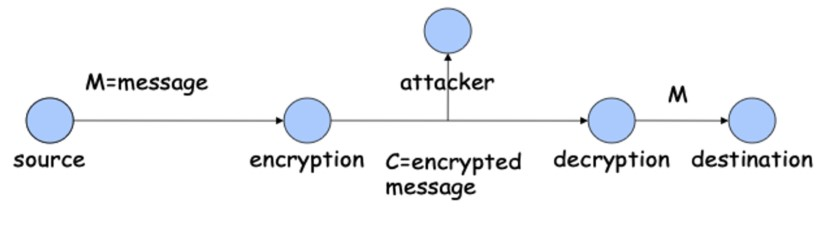
\includegraphics[scale = 1.2]{img/cl1.jpg}
        \label{cl1}
        \caption{First encryption strategy}
    \end{figure}

    An example of this type of encryption is provided by the \textit{Enigma machine}, adopted by the German militaries during World War II;

    \item The \textbf{encryption algorithm is known}, even by the attacker, but Alice and Bob share some information that is not accessible by the attacker (i.e. it travels trough a secure channel), the \textbf{encryption key}.

    \begin{figure}[h!]
        \centering
        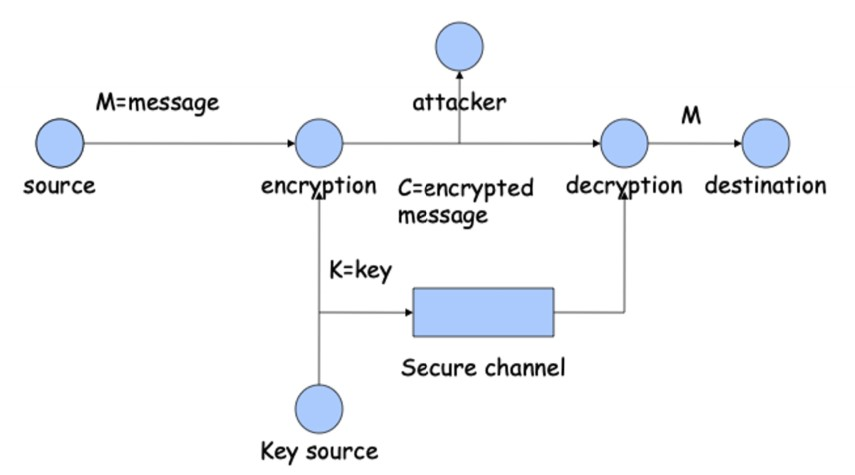
\includegraphics[scale = 1.2]{img/cl2.jpg}
        \label{cl2}
        \caption{Second encryption strategy}
    \end{figure}

    As we can see, in this case both the \textbf{encryption} and the \textbf{decryption} involve the \textbf{secret key} adopted from the source and the destination, and it is usually better than the first strategy, since:

    \begin{itemize}
        \item It is \textbf{simpler} to \textbf{distribute} only one \textbf{key}, rather than an entire encryption algorithm;
        \item If there is an attack, it is \textbf{easier} to \textbf{change key} instead of a whole algorithm.
    \end{itemize}

    For these reasons, this \textbf{second strategy} is \textbf{preferred}.
\end{enumerate}

In general, a \textbf{cryptosystem} (or a \textbf{cipher}) can be defined as a quintuple $(P,C,K,E,D)$, where:

\begin{itemize}
    \item $P$ is the set of \textbf{plaintexts}, i.e. the set of messages we want to share;
    \item $C$ is the set of \textbf{ciphertexts}, i.e. the result of the encryption applied to the plaintexts;
    \item $K$ is the set of \textbf{keys};
    \item $E: k \times P \xrightarrow{} C$ is the \textbf{encryption function}, which takes as input a key and a plaintext, and produces in output an cyphertext;
    \item $D: k \times C \xrightarrow{} P$ is the \textbf{decryption function}, which takes as input a key and a ciphertext, and produces in output a plaintext. Notice that in this case, the input $C$ of the decryption function represents the output of the encryption function.
\end{itemize}

If we consider $x \in P$ (plaintext), $y \in C$ (ciphertext) and $k \in K$, we write $E_k(x)$ and $D_k(y)$ to denote $E(k,x)$ and $D(k,y)$, i.e. the encryption and decryption under the key $k$ of $x$ and $y$, respectively. In this sense, we require that:

\begin{enumerate}
    \item $D(E_k(x)) = x$, i.e. \textbf{decrypting a ciphertext} with the right key gives the \textbf{original plaintext};
    \item Computing $k$ or $x$ given a ciphertext $y$ (which is what the attacker sees, as shown in Picture \ref{cl2}) is \textbf{unfeasible}, meaning that it is so complex that it cannot be done in a reasonable amount of time.
\end{enumerate}

It is important to underline the fact that all the invented ciphers satisfies (1), but some of them do not satisfy (2), as we will see in the following sections.

\subsection{Monoalphabetic ciphers}
We now study some of the most important monoalphabetic ciphers, i.e. ciphers in which the \textbf{letters} of the plaintext are \textbf{mapped} to ciphertext letters based on a \textbf{single alphabetic key}.

\subsubsection{Caesar cipher}
This is probably the \textbf{simplest} and most famous cipher, due to Julius Caesar. The idea is very simple: each \textbf{letter} of a message is \textbf{substituted} with the one that is \textbf{3 positions next} in the alphabet. So, for example, ‘A’ is replaced with ‘D’ and ‘M’ with ‘P’. The substitution can be represented as follows:

\begin{figure}[h!]
        \centering
        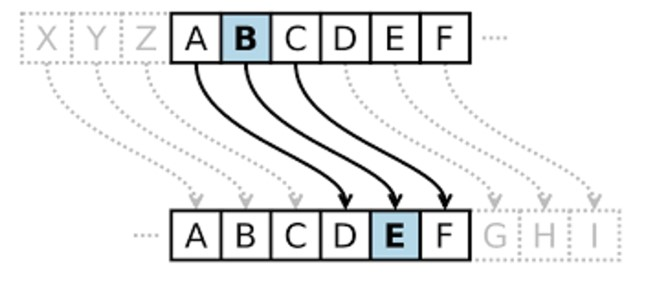
\includegraphics[scale = 1.2]{img/cl3.jpg}
        \label{cl3}
        \caption{Caesar cipher}
\end{figure}

, meaning that each letter in the top alphabet is substituted with the corresponding one in the bottom (rotated) alphabet. For example, the word HOME would be encrypted as KRPH. To \textbf{decrypt} it is enough to apply the \textbf{inverse substitution}.

\begin{figure}[h!]
        \centering
        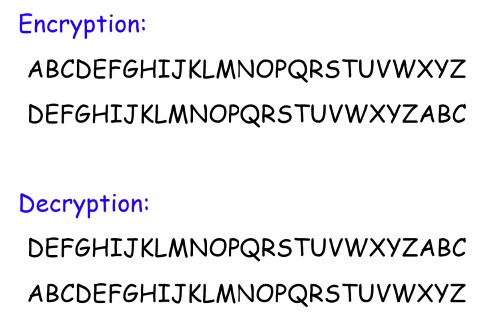
\includegraphics[scale = 1.2]{img/cl4.jpg}
        \label{cl4}
        \caption{Caesar cipher: encryption and decryption}
\end{figure}

In this case:

\begin{enumerate}
    \item The encryption is given by the substitution with the letter in 3 positions next in the alphabet;
    \item The key is 3.
\end{enumerate}

\underline{Example}: we want to decrypt BHV BRX PDGH LW, and we obtain YES YOU MADE IT.

\begin{figure}[h!]
        \centering
        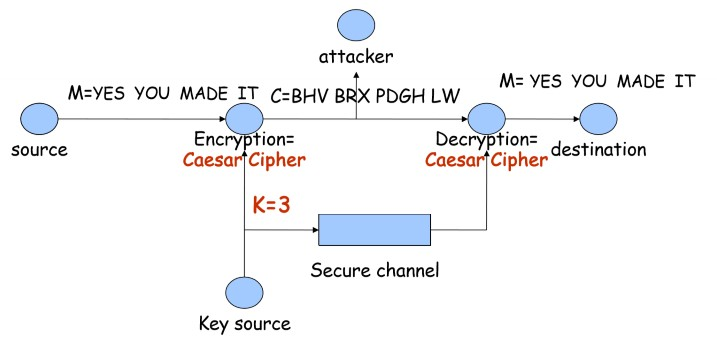
\includegraphics[scale = 1.2]{img/cl5.jpg}
        \label{cl5}
        \caption{Caesar cipher: example}
\end{figure}

Despite being extremely simple, the Ceasar cipher is clearly \textbf{insecure} for many different reasons. First of all, \textbf{once the cipher has been broken} any \textbf{previous} exchanged message is also \textbf{broken}. This is due to the fact that this cipher always works in the same way. There is a famous \textbf{principle} in cryptography, due to Auguste Kerckhoffs, that tells that a \textbf{cipher} should remain \textbf{secure} \textbf{even} if the \textbf{algorithm} becomes \textbf{public}. This is achieved by \textbf{parametrizing} ciphers on a \textbf{key}. The key can be changed and is assumed to be the only secret. This is of course fundamental if we want a cipher to scale and be used by millions of users.

Other Kerckhoffs rules (1883) are:

\begin{enumerate}
    \item The system should be, if not theoretically unbreakable, \textbf{unbreakable in practice};
    \item The \textbf{design} of a system should \textbf{not} require \textbf{secrecy}, and compromise of the system should not inconvenience the correspondents;
    \item The \textbf{key} should be \textbf{memorable} without notes and should be easily changeable;
    \item The cryptograms should be transmittable by a telegraph;
    \item The apparatus or documents should be portable and operable by a single person;
    \item The system should be easy, neither requiring knowledge of a long list of rules nor involving mental strain.
\end{enumerate}

\subsubsection{Shift ciphers}
We now consider a variant of the cipher, called \textbf{shift cipher}, which is parametrized on a key $k$, that we assume to range from 0 to 25. Intuitively, $k$ represents the number of positions in the alphabet that we \textbf{shift} each letter of (since we have 26 letters, we can perform 26 shifts, including the shift of 0 positions). Notice that in this case:

$$
P = C = K = \mathbb{Z}_{26}
$$

, i.e. the plaintexts, the ciphertexts and the keys are the set of integers from 0 to 25. Moreover:

\begin{itemize}
    \item $E_k(x) = (x+k) \mod 26$;
    \item $D_k(y) = (y-k) \mod 26$, where $y = E_k(x)$;
\end{itemize}

Notice that \textbf{Caesar cipher} represents a \textbf{subcase} of \textbf{shift cipher} when $k = 3$.

For example $k$ = 10 gives the following substitution (notice that the bottom alphabet is now shifted to the left by 10 positions):

\begin{figure}[h!]
        \centering
        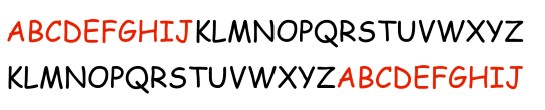
\includegraphics[scale = 1.2]{img/cl6.jpg}
        \label{cl6}
        \caption{Shift cipher: example}
\end{figure}

Does the first property hold? We have to check whether

$$
D_k(E_k(x)) = x
$$

We have that:

$$
D_k((x+k)\mod26) = [(x+k)\mod26 - k]\mod26 = x + (k-k)\mod26 = x\mod26 = x
$$

, so the \textbf{first property} holds. The previous result depends from the fact that $\mathbb{Z}_{26}$ is a group under the addition (not under multiplication). We recall that a group $<G,*>$ is a set $G$ together with a (closed) binary operation $*$ on $G$ s.t.:

\begin{itemize}
    \item The operator is associative, i.e. $(x*y)*z = x*(y*z)$;
    \item There is an element $e \in G$ s.t. $a*e = e*a = e$, the identity element;
    \item For every $a \in G$, there is an element $b \in G$ s.t. $a*b = e$, the inverse element.
\end{itemize}

Notice that $\mathbb{Z}_{26}$ is not closed under multiplication since there's no multiplicative inverse for every element in $\mathbb{Z}_{26}$.

A possible \textbf{attack} for shift cipher is the \textbf{brute force attack}, which consists in trying all the possible 26 keys (i.e. each possible shift): thus, the \textbf{second property does not hold}, since the cipher is \textbf{not secure} if the algorithm becomes public.

\subsubsection{Substitution cipher}
A possible method for overcoming the previous limitation is to consider a \textbf{generic permutation of the alphabet}, so consider a $k$ as a random permutation. Formally, 

$$
P = C = \mathbb{Z}_{26}
$$

and $k = \{\rho|\rho \text{ is a permutation of 0,..,25}\}$. Moreover:

\begin{itemize}
    \item $E_k(x) = \rho(x)$;
    \item $D_k(y) = \rho^{-1}(y)$.
\end{itemize}

An example is provided in Picture \ref{cl7}.

\begin{figure}[h!]
        \centering
        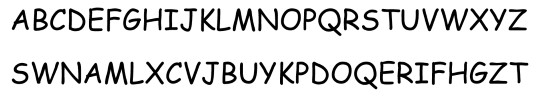
\includegraphics[scale = 1.2]{img/cl7.jpg}
        \label{cl7}
        \caption{Substitution cipher: example}
\end{figure}

Let's see if this cipher satisfy the properties:

\begin{enumerate}
    \item $D_k(E_k(x)) = x$. We have that

    $$
    D_k(\rho(x)) = \rho^{-1}(\rho(x)) = x
    $$
    , so the \textbf{first property is satisfied};
    \item Computing $k$ or $x$ given a ciphertext $y$ is unfeasible. Is the brute force technique still possible in this case? Well, we have 26! possible keys (all the possible permutations of 26 elements), which is approximately $4 * 10^{26} > 2^{88}$, which would be \textbf{unfeasible} even with powerful parallel computers.
\end{enumerate}

However, this cipher is characterized by an important \textbf{limit}, which is of being a \textbf{monoalphabetic cipher}, meaning that it \textbf{maps} a \textbf{letter} \textbf{always} to the very \textbf{same letter}. This preserves the \textbf{statistics} of the plaintext and makes it possible to \textbf{reconstruct the key} by observing the statistics in the ciphertext. For example, vowels e,a,o,i will be easy to identify as they are much more frequent than the other letters.

In this sense, if the attacker knows the used \textbf{cipher} (e.g. monoalphabetic substitution cipher) and the \textbf{language} of the plaintext (e.g. Italian), even without knowing the plaintext and the key he could be able to decrypt the plaintext, by exploiting the statistics of the language of the plaintext. For example, if he knows that the letter S appears 0 times, while letter C appears 15 times, then he can infere that letter C is a transformation of letter A, since it appears a lot of times. For each language we can build a chart of the most frequent letters/bigrams/trigrams, as showed in Picture \ref{cl8_9}.

\begin{figure}[h!]
        \centering
        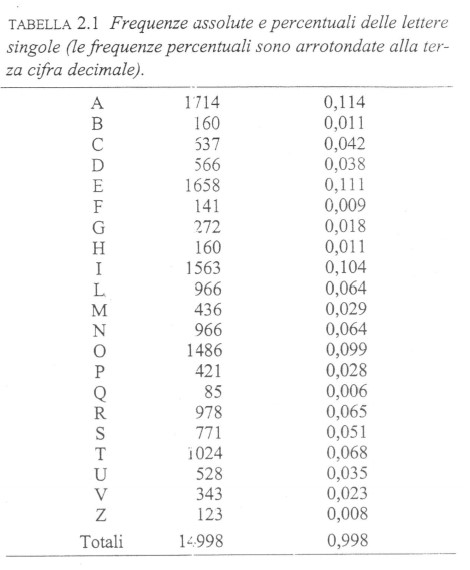
\includegraphics[scale = 1.2]{img/cl8.jpg}
        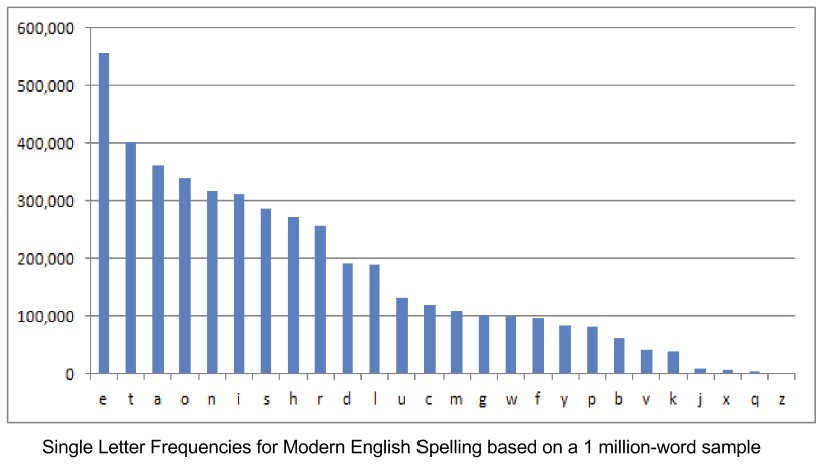
\includegraphics[scale = 1.2]{img/cl9.jpg}
        \label{cl8_9}
        \caption{Language statistics}
\end{figure}

Other deductions can be made from the fact that, for example, in Italian the frequency of letter I and L increases at the beginning of the sentences, while the one of A,E,I,O,U at the end of the words etc.. 

In this sense, a possible approach for decrypting a monoalphabetic substitution cipher could be the following:

\begin{enumerate}
    \item We \textbf{order} the letters of the ciphertext into decreasing frequencies;
    \item We \textbf{substitute} with letters in decreasing order as in the corresponding tables (depending on the language), by eventually exchanging letters with similar frequencies and by also exploiting digraphs and trigraphs frequently used,
\end{enumerate}

\subsection{Polyalphabetic ciphers}
We have seen that \textbf{monoalphabetic} ciphers are prone to \textbf{statistical attacks}, since they preserve the statistical structure of the plaintext. To overcome this issue, it is important that the same plain symbol is not always mapped to the same encrypted symbol. When this happens the cipher is called \textbf{polyalphabetic}.

\subsubsection{Vigenére cipher}
This simple polyalphabetic cipher works on \textbf{“blocks”} of $m$ letters with a key of length $m$. For example, if we consider the text "THISISAVERYSECRETMESSAEG" and the key "FLUTE", the plaintext is splitted into blocks of length 5, and the key FLUTE is repeated as necessary and used to encrypt each block, as showed in Picture \ref{poly1}.

\begin{figure}[h!]
        \centering
        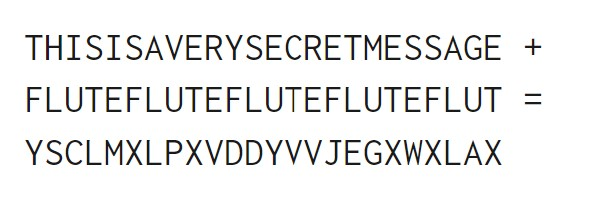
\includegraphics[scale = 1.2]{img/poly1.jpg}
        \label{poly1}
        \caption{Vigenére cipher: example}
\end{figure}

Formally, $P = C = K = \mathbb{Z}_{26}^m$, where $\mathbb{Z}_{26}^m$ is $\mathbb{Z}_{26}\times\mathbb{Z}_{26}\times\ldots\times\mathbb{Z}_{26}$, $m$ times. Encryption and decryption are defined as follows:

\begin{itemize}
    \item $E_{k1, .., km}(x_1, .., x_m) = (x_1 + k_1, .., x_m + k_m)\mod26$;
    \item $D_{k1, .., km}(y_1, .., y_m) = (y_1 - k_1, .., y_m - k_m)\mod26$
\end{itemize}

In the example above, $k_1 = \text{F}$, $k_2 = \text{L}$ etc..

The first \textbf{strength} of this cipher is that since the \textbf{number of possible keys} is $26^m$ (i.e. the number of possible keys is given by the total number of possible sequences of $m$ letters), for $m$ big enough this \textbf{prevents} \textbf{brute force attacks}. Another strength is given by the fact that \textbf{one letter} is \textbf{not always mapped} to the \textbf{same one} (unless the are at a distance that is multiple of $m$). For example the fist two letters “I” are encrypted as “C” and “M”, respectively. While the “S” in position 6 and the last one are both encrypted as “X” using the “F” of “FLUTE”. They are, in fact, at distance 15 which is a multiple of 5. Thus, the \textbf{histogram} of the \textbf{frequencies} is \textbf{flat}, and the flatness increases with the increase of the key length. 

\paragraph{Breaking Vigenére cipher: the Friedman method} Even if Vigenére cipher hides the statistic structure of the plaintext better than monoalphabetic ciphers, it still preserve most of it. There are two famous methods to break this cipher. The first is due to Friedrick Kasiski (1863) and the second to Wolfe Friedman (1920). We illustrate the latter since it is more suitable to be mechanized. Both are based on the following steps:

\begin{enumerate}
    \item Recover the \textbf{length} $m$ of the \textbf{key}. The intuition is that once we know $m$, we know that at distance $m$ we'll find the same letter of the key, thus the letters at distance $m$ form a monoalphabetic cipher;
    \item Recover the \textbf{key}.
\end{enumerate}

\textbf{STEP 1: recover \textit{m}}

The Friedman method uses statistical measures to recover the length $m$ of the key. In particular, we consider the \textbf{index of coincidence}, which is defined as:

$$
I_c(x) = \frac{\sum_{i = 1}^{26} f_i (f_i - 1)}{n (n-1)} \approx \sum_{i = 1}^{26} p_i^2
$$
, where:

\begin{itemize}
    \item $x$ represents the text for which the index of coincidence is computed;
    \item $f_i$ represents the frequency of the $i$-th letter in the text;
    \item $n$ is the length of the text;
    \item $p_i$ represents the probability of the $i$-th letter, and it is computed as $p_i = \frac{f_i}{n}$.
\end{itemize}

Intuitively, the index of coincidence measures the \textbf{probability} that \textbf{two letters}, chosen at \textbf{random} from the text $x$, are the \textbf{same}. Indeed, the index is computed by multiplying the probability that the first letter is the $i$-th ($\frac{f_i}{n}$) and the probability that the second letter is the $i$-th ($\frac{f_i - 1}{n-1}$): in this case we subtract 1 since the first letter has been already fixed).

\underline{Example}: we compute the index of coincidence of the text "the index of coincidence". We have that:

$$
\frac{\text{c}(3 * 2) + \text{d}(2 * 1) + \text{e}(4 * 3) + \text{f}(1 * 0) + \text{h}(1 * 1) + ...}{21 * 20} = 0.0809
$$

If we consider the random text "bmqvszfpjtcsswgwvjlio", the index has value $0.0286$: as we can see, the index of coincidence of a random sentence is smaller that the one of a normal sentence. 

More specifically, notice that the \textbf{value} of the index is \textbf{minimum}, with value $1/26 \approx 0.038$, for texts composed of \textbf{letters} chosen with \textbf{uniform probability} $1/26$ while it is \textbf{maximum}, with value $1$, for texts composed of just a \textbf{single letter} repeated $n$ times. It is, in fact, a \textbf{measure} of how \textbf{non-uniformely letters} are \textbf{distributed} in a \textbf{text}. For this reason, each \textbf{natural language} has a characteristic \textbf{index of coincidence}: for English the value is approximately $0.065$. 

In general, using frequencies analysis, we saw that if \textbf{frequencies} are \textbf{flat} we have a \textbf{polyalphabetic cipher}, if we have \textbf{peaks} and valleys of frequencies we have a \textbf{monoalphabetic cipher}. If the \textbf{value} of the \textbf{index of coincidence} is \textbf{minimum} ($\approx 0.038$) we have a \textbf{polyalphabetic cipher}, if it is $\approx 0.065$ we have a \textbf{monoalphabetic cipher} (same as English, just a permutation of letters).

Now the question is: how do we recover the length $m$ of the key using the Friedman method, and in particular the concept of index of coincidence? Well, the idea is to find the length by brute-forcing, following this algorithm:

\begin{figure}[h!]
        \centering
        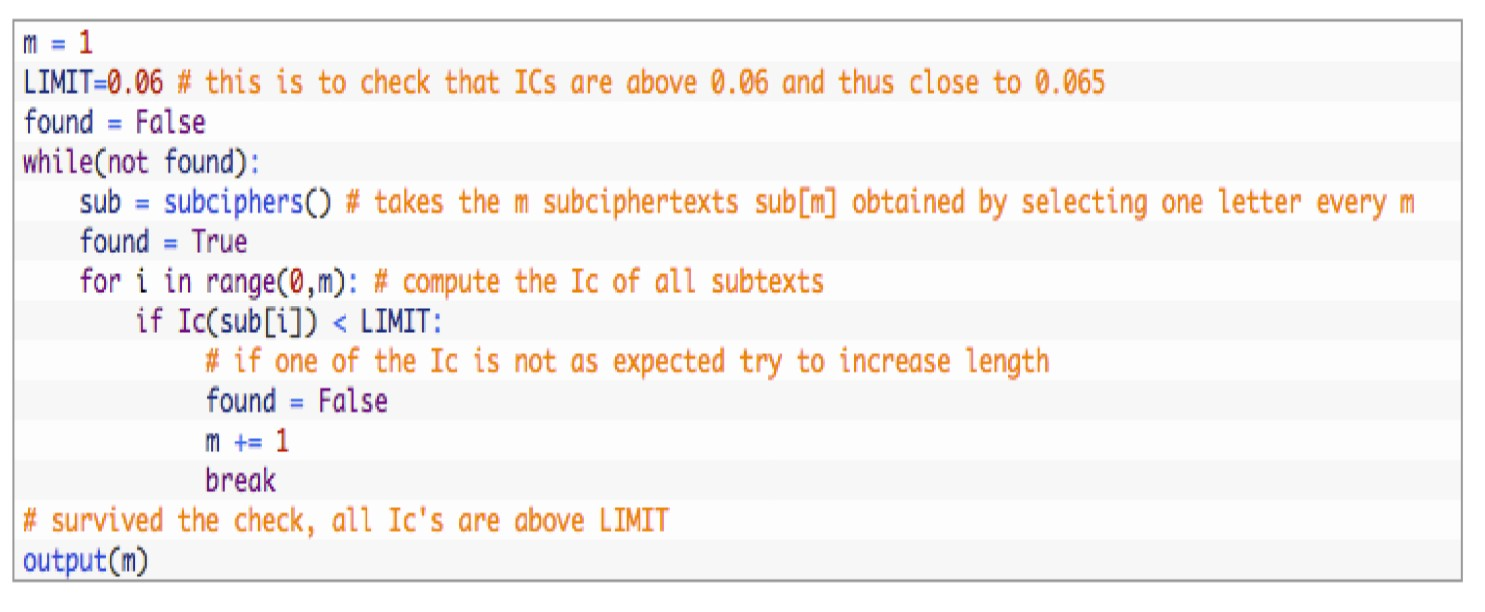
\includegraphics[scale = 0.9]{img/poly2.jpg}
        \label{poly2}
        \caption{Friedman method: estimating $m$}
\end{figure}

As we can see, the idea of the algorithm is the following:

\begin{enumerate}
    \item We \textbf{initialize} the value of $m$ to 1 (a value $m = 0$ does not make sense);
    \item We consider the $m$ \textbf{sub-ciphertexts} obtained by selecting one letter every $m$ (e.g. for $m = 2$ we get the two sub-ciphertexts composed of only the letters in odd positions and even positions, respectively);
    \item Then, we compute the \textbf{index of coincidence} of all the sub-ciphertexts, increasing the value of $m$ if the current index has a value smaller than $0.065$ (the IC of the English language). We require that the index of coincidence of all the subtexts is close to the characteristic index of the plaintext language. Typically, the bigger is the index the higher is the probability that the frequencies of the letters are close to the one of the plaintext language. It is thus enough to choose a lower bound such as 0.06 and check that the ICs are above that;
    \item The loops stops when $IC(\text{sub-ciphertext}) \geq 0.065$.
\end{enumerate}

\textbf{STEP 2: recover the key}
Once we have found the length $m$ of the key, we need to \textbf{find the key}. We consider a \textbf{text} composed of \textbf{letters} at \textbf{distance} $m$ from the first one, and the ones at distance $m$ from the second one. They have different shifts, how can we find the \textbf{relative right shift}? An example is provided in Picture \ref{poly3}.

\begin{figure}[h!]
        \centering
        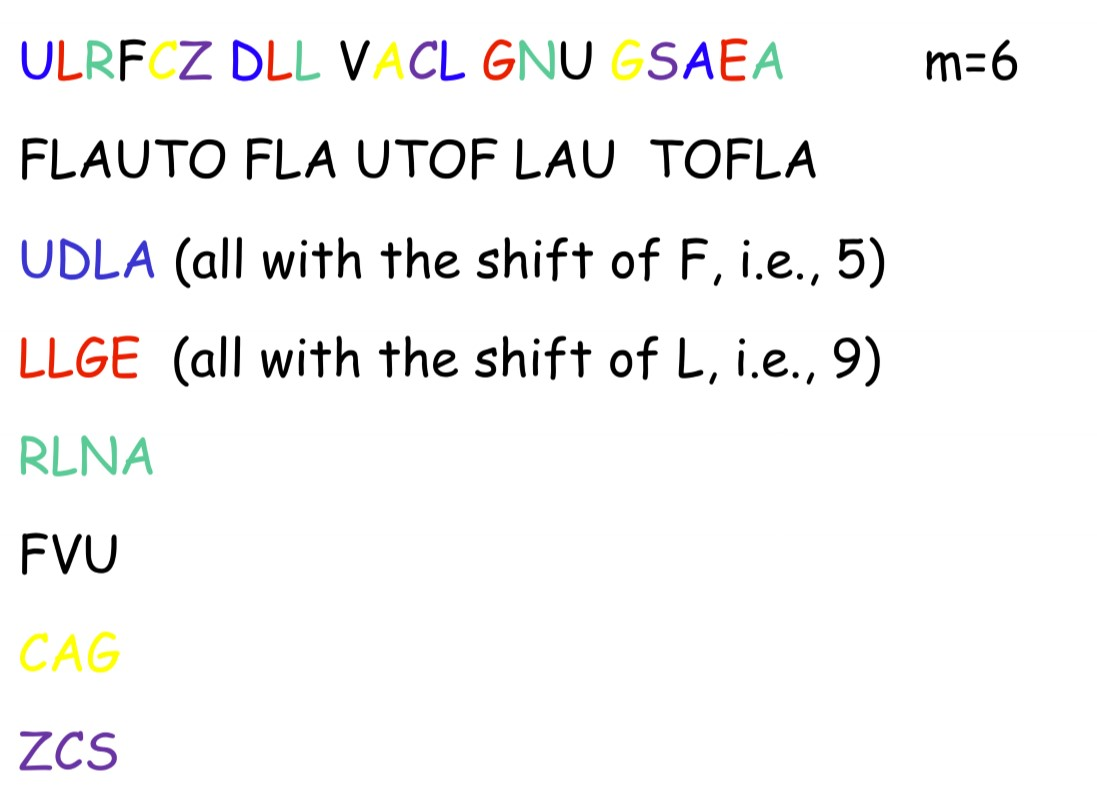
\includegraphics[scale = 0.75]{img/poly3.jpg}
        \label{poly3}
        \caption{Examples of shifts}
\end{figure}

Our goals now are:

\begin{enumerate}
    \item Determine the \textbf{shift} between the first letter of the key and the other $m-1$ letters;
    \item Determine the \textbf{first letter} (brute force on 26 possible letters) and, by exploiting the shifts we've just computed, determine the remaining letters of the key.
\end{enumerate}

We find the \textbf{relative shift} between two sub-ciphers by using the \textbf{mutual index of coincidence}, which is defined as:

$$
MI_c (x,x') = \frac{\sum_{i = 1}^{26} f_i f_i'}{n n'} = \sum_{i = 1}^{26} p_i p_i'
$$
, where:

\begin{itemize}
    \item $x$ represents the first text for which the mutual index of coincidence is computed;
    \item $x'$ represents the second text for which the mutual index of coincidence is computed;
    \item $f_i$ represents the frequency of the $i$-th letter in the text $x$;
    \item $f_i'$ represents the frequency of the $i$-th letter in the text $x'$;
    \item $n$ is the length of the text $x$;
    \item $n'$ is the length of the text $x'$;
    \item $p_i$ represents the probability of the $i$-th letter in text $x$, and it is computed as $p_i = \frac{f_i}{n}$;
    \item $p_i'$ represents the probability of the $i$-th letter in text $x'$, and it is computed as $p_i' = \frac{f_i'}{n'}$.
\end{itemize}

Intuitively, the mutual index of coincidence represents the \textbf{probability} that \textbf{two letters} taken from two texts $x$ and $x'$ are the \textbf{same}. 

The idea is to \textbf{shift one sub-cipher} until the \textbf{mutual index} of coincidence with the first sub-cipher becomes \textbf{close} to the one of the plaintext language. When this happens, we know that the applied shift is the relative shift between the two sub-ciphers and, consequently, between the corresponding letters of the key. This is encoded in the following algorithm. In fact, what we do, is to select the relative shift that maximizes the mutual index of coincidence.

\begin{figure}[h!]
        \centering
        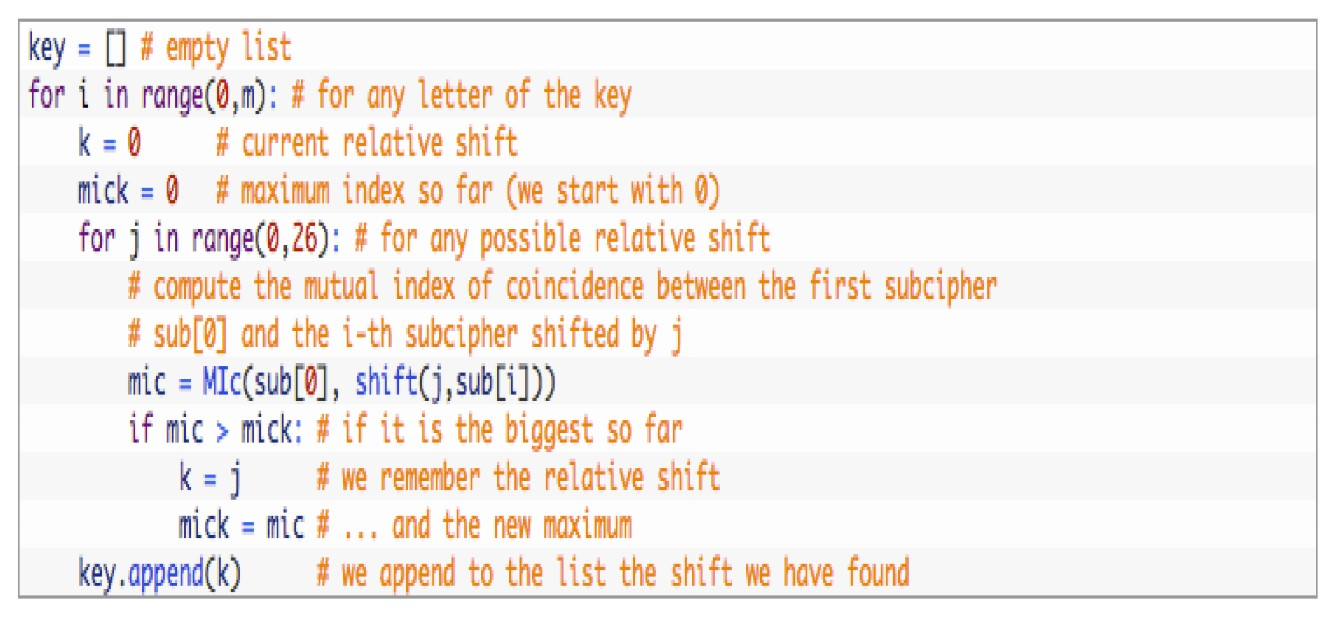
\includegraphics[scale = 0.9]{img/poly4.jpg}
        \label{poly4}
        \caption{Friedman method: finding the key}
\end{figure}

We \textbf{repeat} this \textbf{for each letter of the key}, and we obtain the \textbf{list of relative shifts}. For example key = [0,4,6,3,9] means that the second letter of the key is equal to the first plus 4 while the third is the first plus 6 and so on. The final step is to try all the possible 26 first letter of the key, giving 26 possible keys (this step could be avoided computing the MIc with a reference text written in the plaintext language).

\subsubsection{Properties}
In general, polyalphabetic ciphers are more \textbf{difficult} to be \textbf{decrypted}, but still are \textbf{not strong enough} (we presented a method for attacking Vigenére cipher).

\subsection{Known-plaintext attacks}
So far, we have considered \textbf{attackers} that \textbf{only know the ciphertext} $y$ and try to \textbf{find} either the \textbf{plaintext} $x$ or the \textbf{key} $k$. In practice, it is often the case that an \textbf{attacker} can \textbf{guess part of the plaintext}. Think of encrypted messages: a message always have a standard header in a certain format and it is often easy to guess part of the information in it. Thus if a message is split into blocks which are encrypted under the same key, it is reasonable to assume that an attacker can deduce part of the plaintext. Also, if a key is reused to encrypt many plaintexts, it can occur that in the future one of the plaintext is leaked (because its security is no more relevant). This gives the attacker knowledge of a pair $(x,y)$ \textbf{plaintext, ciphertext}.

For these reasons, in cryptography we often consider so-called \textbf{known-plaintext attacks}, i.e., we assume the attacker knows some pairs $(x’,y’), (x'',y''), ..$ of plaintexts/ciphertexts. The challenge, given $y$, is to find the relative $x$ or the $k$. We illustrate this kind of attacks on a classical cipher.

In general, the possible attacks we can consider are:

\begin{itemize}
    \item \textbf{Ciphertext-only attacks}: in a ciphertext-only attack the \textbf{attacker} is \textbf{assumed} to have access only to a set of \textbf{ciphertexts} (e.g., monoalphabetic ciphers, polyalphabetic ciphers). In this case the \textbf{limit} is that it is \textbf{easy to find} the \textbf{correspondence} between \textbf{letters} in the \textbf{plaintext} and in the \textbf{ciphertext};
    \item \textbf{Known-plaintext attacks}: the attacker knows some \textbf{pairs} $(x',y'), (x'', y''), ..$ of plaintexts/ciphertexts;
    \item \textbf{Chosen-plaintext attack (CPA)}, which presumes that the attacker can ask and obtain the \textbf{ciphertexts} for \textbf{given plaintexts};
    \item \textbf{Chosen-ciphertext attack (CCA)}, where the cryptanalyst can gather information by obtaining the \textbf{decryptions} of \textbf{chosen ciphertexts}. 
\end{itemize}

\subsubsection{The Hill cipher}
This cipher is polyalphabetic and generalizes the idea of Vigenére by introducing \textbf{linear transformations} of blocks of plaintext. 

Formally, ${\cal P} = {\cal C} = \mathbb{Z}_{26}^m$, while ${\cal K} = \{ K \ | \ K  \text{ is an invertible mod 26 } m\times m \text{ matrix} \}$. Encryption and decryption are defined as follows:

\begin{itemize}
    \item $E_k (x_1, .., x_m) = (x_1, .., x_m) K \mod 26$, i.e. we multiply the message and the matrix, modulo 26;
    \item $D_k (y_1, .., y_m) = (y_1, .., y_m) K^{-1} \mod 26$, i.e. we multiply the encrypted message and the inverse of the matrix, modulo 26.
\end{itemize}

\underline{Example}: let us assume $M = \text{message } = (x_1, x_2) = (5,9)$, and $
K = \begin{bmatrix}
5 & 11 \\
8 & 3 
\end{bmatrix}
$

To \textbf{encrypt} $M$, we have to:

\begin{itemize}
    \item Take $M = (x_1, .., x_m)$ and $K$ which is a \textbf{matrix};
    \item Compute $(x_1,...,x_m) K \mod 26$.
\end{itemize}

Thus, $E_k (5,9) = (5,9) * \begin{bmatrix}
5 & 11 \\
8 & 3 
\end{bmatrix} \mod 26 = (25 + 72, 55 + 27) \mod 26 = (19,4)$

To \textbf{decrypt} $M$, we have to:

\begin{itemize}
    \item Compute the \textbf{inverse} of $K$, i.e., $K^{-1}$ ($K$ is invertible);
    \item Compute $(y_1, .., y_m) K^{-1} \mod 26$.
\end{itemize}

The \textbf{inverse} of $K$ is computed as:

$$
K^{-1} = \text{det}^{-1}(K) \begin{bmatrix}
3 & -11 \\
-8 & 5 
\end{bmatrix} \mod 26 = \text{det}^{-1} (K) \begin{bmatrix}
3 & 15 \\
18 & 5 
\end{bmatrix} \mod 26
$$

Now,

$$
\text{det}(K) = (15 - 88) \mod 26 = 5
$$

, and to compute $\text{det}^{-1} (K)$ (i.e. the inverse mod 26 of 5) we need to find a number in the interval [0,25] that multiplied by 5 mod 26 gives 1. In this case the number is 21 ($5 * 21 \mod 26 = 1$). Thus, $\text{det}^{-1} (K) = 21$. Notice that it is not always the case that the multiplicative inverse modulo exists. We will discuss this more in detail when introducing public key cryptography and RSA. We now have to solve:

$$
K^{-1} = \text{det}^{-1} (K) \begin{bmatrix}
3 & 15 \\
18 & 5 
\end{bmatrix} \mod 26 = 21 \begin{bmatrix}
3 & 15 \\
18 & 5 
\end{bmatrix} \mod 26 = \begin{bmatrix}
63 & 315 \\
378 & 105 
\end{bmatrix} \mod 26 = \begin{bmatrix}
11 & 3 \\
14 & 1 
\end{bmatrix}
$$

Thus, 

$$
D_k(19,4) = (19,4) * \begin{bmatrix}
11 & 3 \\
14 & 1 
\end{bmatrix} \mod 26 = (265, 62) \mod 26 = (5,9)
$$

Assume, now, that the \textbf{attacker} knows (at least) $m$ \textbf{pairs} of plaintexts/ciphertexts, where $m$ is the block length, and his goal is to \textbf{find} the relative $x$ or $k$ given $y$. We know that:

\begin{align*}
    (y_1^1, .., y_m^1) = (x_1^1, .., x_m^1) K \mod 26 \\ 
    \hdot \\
(y_1^m, .., y_m^m) = (x_1^m, .., x_m^m) K \mod 26
\end{align*}

, where each $x^i$ represents a plaintext, and each $y^i$ represents a ciphertext. Moreover, the previous system of equations can be written as:

$$
Y = XK \mod 26
$$

, where $X = \begin{bmatrix}
x_1^1 & \hdots & x_m^1 \\
\hdots & \ddots & \hdots \\
x_1^m & \hdots & x_m^m
\end{bmatrix}$ and $Y = \begin{bmatrix}
y_1^1 & \hdots & y_m^1 \\
\hdots & \ddots & \hdots \\
y_1^m & \hdots & y_m^m
\end{bmatrix}$. 

It is now clear that if $X^{-1}$ exists, we obtain:

$$
X^{-1}Y \mod 26 = X^{-1} X K \mod 26
$$

, but $X^{-1}X = 1$, so $K = X^{-1}Y \mod26$.

The \textbf{Hill cipher} is a \textbf{linear transformation of a plaintext block} into a \textbf{cipher block}. The above attack shows that this kind of \textbf{transformation} is \textbf{easy to break} if enough \textbf{pairs} of \textbf{plaintexts} and \textbf{ciphertexts} are \textbf{known}. \textbf{Modern ciphers}, in fact, always contain a \textbf{non-linear component} to prevent this kind of attacks.

\underline{Example}: assume that the attacker has the pairs $(5,9) \xrightarrow{} (19,4)$ and $(2,5) \xrightarrow{}(24,11)$, and $m = 2$. How can we find $K$? Firstly, we need to compute $X^{-1}$: if this matrix exists, we can derive $K$ from the formula above.

\begin{equation*}
    \begin{align*}
        X^{-1} &= \text{det}(X)^{-1} \begin{bmatrix}
5 & -9 \\ -2 & 5 
\end{bmatrix} \mod 26 \\ &= \text{det}(X)^{-1} \begin{bmatrix}
5 & 17 \\
24 & 5 
\end{bmatrix} \mod 26 \\ &= 15  \begin{bmatrix}
5 & 17 \\
24 & 5 
\end{bmatrix} \mod 26 \\ &= \begin{bmatrix}
23 & 21 \\
22 & 23 
\end{bmatrix}      
    \end{align*}
\end{equation*}

Then, $K = X^{-1}Y \mod 26 = \begin{bmatrix}
23 & 21 \\
22 & 23 
\end{bmatrix} \begin{bmatrix}
19 & 4 \\
24 & 11 
\end{bmatrix} \mod 26 = \begin{bmatrix}
5 & 11 \\
8 & 3 
\end{bmatrix}$

\subsection{Euclidean algorithm}
We now consider an \textbf{algorithm} for computing in an \textbf{efficient} way the operation of \textit{inverse modulo $n$}. We begin by introducing the \textbf{Euclidean algorithm}, which is used to computed $\text{gcd}(c,d)$ represented in Picture \ref{eu1}.

\begin{figure}[h!]
        \centering
        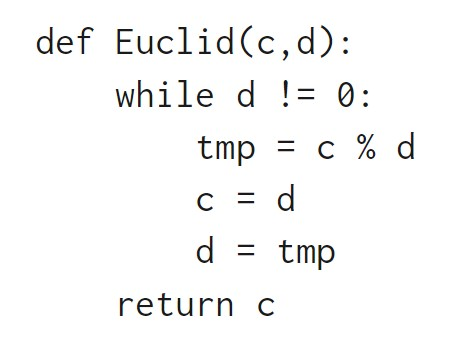
\includegraphics[scale = 0.9]{img/eu1.jpg}
        \label{eu1}
        \caption{Euclidean algorithm}
\end{figure}

In this case, the idea is that, to compute $\text{gcd}(c,d)$, when $d \neq 0$, we can compute $\text{gcd}(d,c \mod d)$, since it can be easy seen that they're the same.

\underline{Example}: $\text{gcd}(5,15) = 5$

This algorithm terminates in $O(k^3)$, given that the \textbf{number of iterations} is $O(k)$. This latter fact can be proved by observing that every 2 steps we at least halve the value $d$. Assume by contradiction that after one step this is not true, i.e., $c \mod d > \frac{d}{2}$. Next step will compute $d \mod (c \mod d) = d - (c \mod d) < \frac{d}{2}$ giving the thesis. We know that halving leads to a logarithmic complexity, i.e., linear with respect to the number of bits $k$.

We now \textbf{extend} the \textbf{algorithm} so to compute the \textbf{inverse modulo} $d$ whenever $gcd(c,d)=1$. We substitute the computation of $c\mod d$ with:

$$
q = c/d
$$

, i.e. an integer division, and

$$
\text{tmp} = c - qd
$$

, which represents the operation $c \mod d$.

\underline{Example}: $12 \mod 5 = 2$, $q = \frac{12}{5}$ and $\text{tmp} = 12 - 2*5 = 2$.

We add two extra variables $e$ and $f$ and we save the initial value of $d$ in $d_0$, as follows:

\begin{figure}[h!]
        \centering
        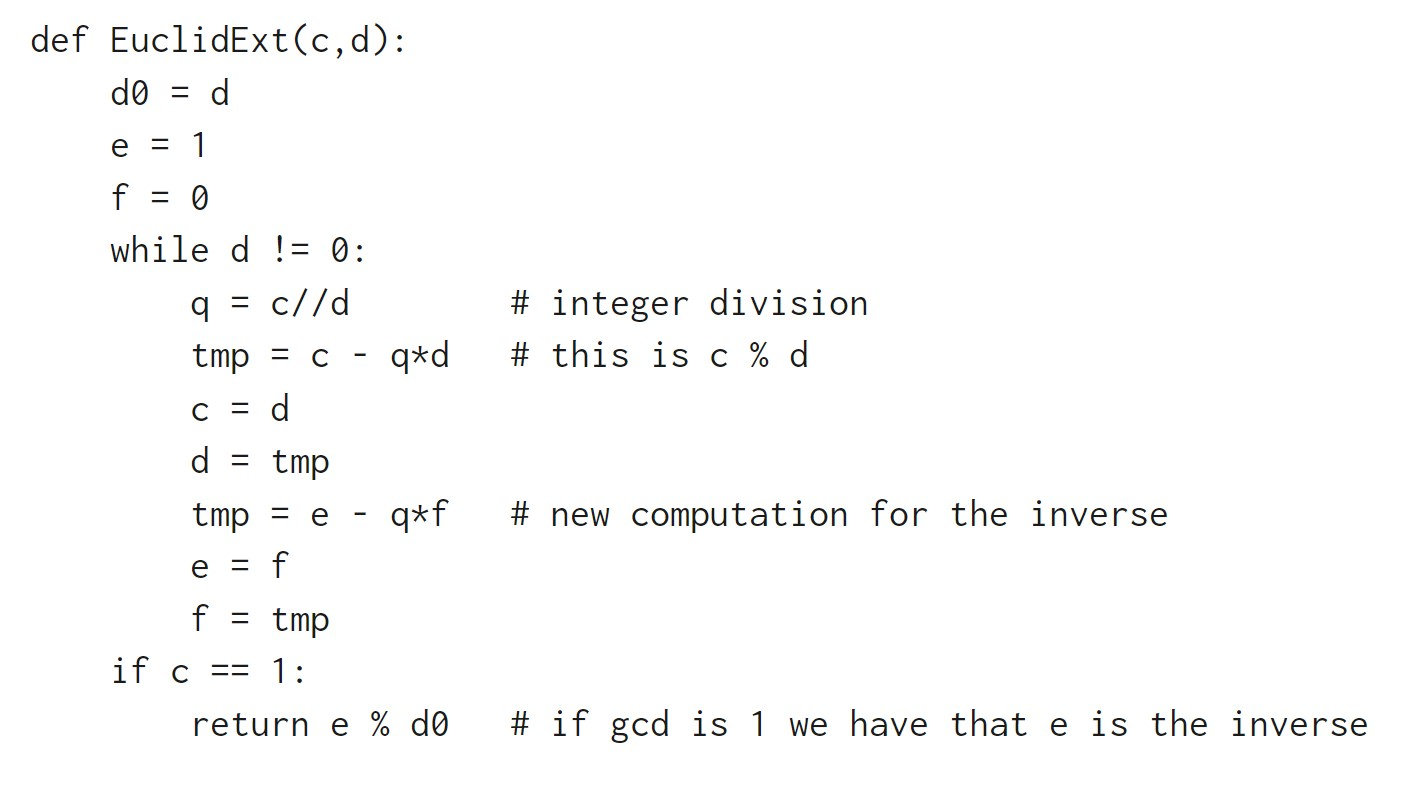
\includegraphics[scale = 0.9]{img/eu2.jpg}
        \label{eu2}
        \caption{Extended euclidean algorithm}
\end{figure}

\underline{Example}: the inverse between 5 and 17 can be computed using $\text{EuclidExt}(5,17) = 7$.

\subsection{Stream ciphers}
So far, we have illustrated cryptosystems that “reuse” the same key to encrypt letters or blocks of the plaintext. This is usually referred to as \textbf{block ciphers}.

\begin{figure}[h!]
        \centering
        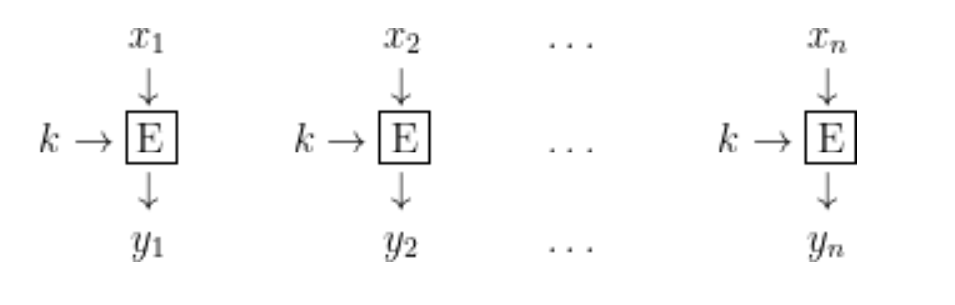
\includegraphics[scale = 1.0]{img/stream1.png}
        \label{stream1}
        \caption{Block cipher}
\end{figure}

This scheme can be \textbf{generalized} by considering a \textbf{stream of keys} instead of a fixed one. Let $z_1, z_2, \ldots, z_n$ be such a stream. The idea is to \textbf{encrypt} the \textbf{first letter} of the plaintext with $z_1$, the \textbf{second} with $z_2$ and so on. It does not matter much if we encrypt a letter or a block, the important difference is that the used key is always different.

\begin{figure}[h!]
        \centering
        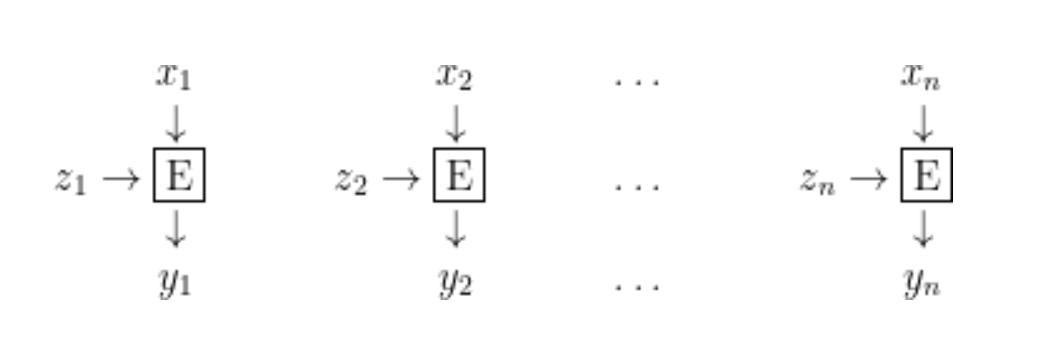
\includegraphics[scale = 1.0]{img/stream2.png}
        \label{stream2}
        \caption{Cipher using different keys}
\end{figure}

Having a \textbf{different key} for \textbf{each letter} or block of the plaintext is of course \textbf{appealing} but \textbf{not} much \textbf{practical}. The stream of key is thus usually derived starting from an initial key $k$. To make the \textbf{stream more complex} it can also \textbf{depend} on \textbf{previous part of the plaintext}. In general we say that 

$$z_i = f_i(k,x_1,\ldots,x_{i-1})$$

, i.e. the $i$-th key depends on $k$ and on the previous $i-1$ letters (or blocks).

To understand why a key $z_i$ cannot depend on plaintexts with indexes greater than or equal to $i$, it is useful to reason on the decryption scheme:

\begin{figure}[h!]
        \centering
        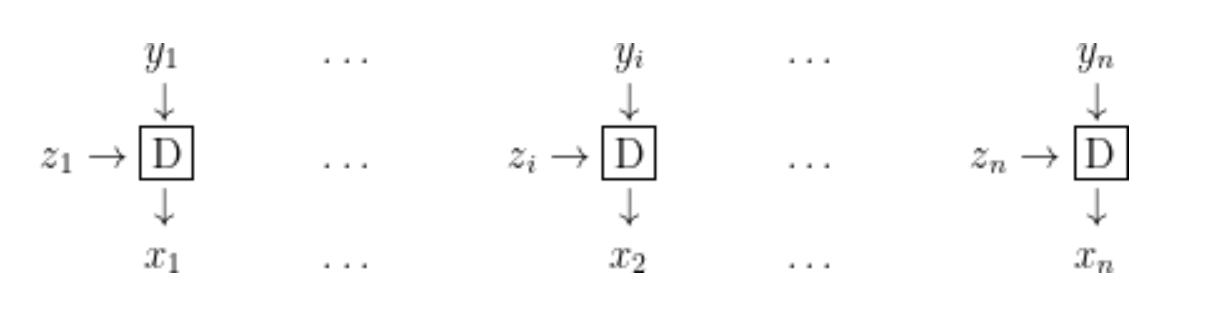
\includegraphics[scale = 1.0]{img/stream3.png}
        \label{stream3}
        \caption{Decryption of a cipher using different keys}
\end{figure}

Now, $z_1 = f_1(k)$ meaning that we can compute it with not knowledge of the plaintext. To compute $z_2 = f_2(k,x_1)$, instead, we need to know $x_1$. As a consequence, we have to decrypt $y_1$ with $z_1$ before computing $z_2$. Once we have this key we can decrypt $x_3$ and compute $z_3$, and so on. The values are thus computed in the following sequence: $z_1,x_1,z_2,x_2, \ldots, z_n,x_n$. It should be evident, now, that we cannot let $z_i$ depend, e.g., on $x_i$ as we would need that plaintext to compute the key.

Notice that \textbf{block ciphers} are, clearly, a \textbf{simple instance} of \textbf{stream ciphers} where $z_i = k$ for all $i$. It is also useful to classify these ciphers depending on certain properties of the key stream:

\begin{itemize}
    \item \textbf{Periodic} stream ciphers;
    \item \textbf{Synchronous} stream ciphers;
    \item \textbf{Asynchronous} stream ciphers;
\end{itemize}

\subsubsection{Periodic stream ciphers}
A stream cipher is \textbf{periodic} if its key stream has the following form $z_1,z_2,\ldots,z_d,z_{1},z_2,\ldots,z_d,z_1\ldots$, i.e., if it \textbf{repeats} after $d$ steps.

Note that \textbf{Vigenére ciphers} can be seen as a \textbf{stream cipher} acting on \textbf{single letters} and with a \textbf{periodic key stream}. For example, if we want to formalize the cipher giving $({\cal P},{\cal C},{\cal K},E,D)$  and defining the key stream $z_i$, we have that:

\begin{itemize}
    \item $E_{z_i}(x_i)=(x_i+z_i) \mod 26$;
    \item $D_{z_i}(y_i)=(y_i-z_i) \mod 26$;
    \item $z_i = k_{i \mod m}$.
\end{itemize}

\subsubsection{Synchronous stream ciphers}
A stream cipher is \textbf{synchronous} if its \textbf{key stream does not depend on plaintexts}, i.e., $z_i = f_i(k)$ for all $i$. When this happens, we have that the key stream can be generated starting from $k$ and independently on the plaintext. This is particularly useful to improve efficiency: we do not need to obtain $x_{i}$ to compute $z_{i+1}$. In fact, the key stream can be generated offline, before the actual ciphertext is received.

As an example, \textbf{Vigenére ciphers} can be seen as a \textbf{synchronous stream cipher}.

\subsubsection{Asynchronous stream ciphers}
This is the general case where $z_i = f_i(k,x_1,\ldots,x_{i-1})$. As mentioned above, we need to decrypt and compute the keys stream at the same time, as a key can depend on previous plaintexts. 

We give a simple example of a cipher of this class, called \textbf{Autokey}. We let ${\cal P}={\cal C}={\cal K}=\mathbb{Z}_{26}$. $E_z(x) = x+z \mod 26$ and $D_z(y) = y-z \mod 26$, i.e., \textbf{encryption} and \textbf{decryption} are exactly as in a \textbf{shift cipher}. The key stream is defined as $z_1 = k$ and $z_i = x_{i-1}$ for $i\geq 2$, meaning that the first key in the stream is the initial key k while the next keys are the same as the previous plaintext.

\begin{figure}[h!]
        \centering
        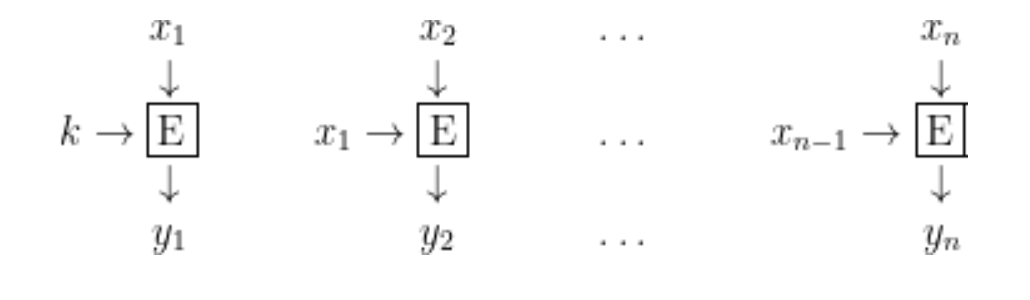
\includegraphics[scale = 1.0]{img/stream4.png}
        \label{stream4}
        \caption{Autokey cipher}
\end{figure}

\underline{Example}: consider the autokey cipher, and assume that the plaintext is the word "networksecurity", what is the encryption using $k = 5$ (recall: $E_z(x) = x+z \mod 26$)? The corresponding numbers are 13, 4, 19, 22, 14, 17, 10, 18, 4, 2, 20, 17, 8, 19, 24, so the encryption is $z_1 = 5$, $z_2 = x_1 = 13$, $z_3 = x_2 = 4$ etc.., so the result numbers are 18, 17, 23, 15, 10, 5, 1, 2, 22, 6, 22, 11, 25, 1, 17, and the corresponding ciphertext is SRXPKFBCWGWLZBR. For the encryption, we have that $D_z(y) = y-z \mod 26$, so we can use $k = 5$ to find the first letter $x_1$ of the plaintext: $x_1 = (18-5) \mod 26 = 13$. Then, we can use $x_1$ as a key to find $x_2$ : $x_2 = (17-13) \mod 26 = 4$ etc..

Notice that the \textbf{autokey} cipher is \textbf{insecure}, since there are only 26 different keys.

\subsection{Perfect ciphers}
We now discuss a \textbf{theoretical result} on the security of cryptosystems. We ask whether \textbf{perfect ciphers} exists, i.e., ciphers that can never be broken, even with after an unlimited time (informal definition). Interestingly, we will see that these ideal ciphers \textbf{exist} and \textbf{can be implemented in practice} but they are, in fact, \textbf{unpractical}. The theory, developed by \textbf{Claude Shannon}, assumes an \textbf{only-ciphertext} model of the \textbf{attacker}, i.e., the attacker only knows the ciphertext $y$ and tries to find plaintext $x$ or key $k$.

Another informal definition of perfect cipher is the following: a cipher system is said to offer perfect secrecy if, on \textbf{seeing} the \textbf{ciphertext} the interceptor gets \textbf{no extra information} about the \textbf{plaintext} than he had before the ciphertext was observed. In a cipher system with perfect secrecy the interceptor is “forced” to guess the plaintext.

\subsubsection{Probability distribution}

We call:

\begin{itemize}
    \item $p_{\cal P}(x)$ the \textbf{probability} of a \textbf{plaintext} $x$ to occur;
    \item $p_{\cal K}(k)$ the \textbf{probability} of a certain \textbf{key} $k$ to be used as encryption key.
\end{itemize}

These two probability distributions induce a \textbf{probability distribution} on the \textbf{ciphertexts}. In fact, given a plaintext and a key there exists a unique corresponding ciphertext. We can compute such a probability distribution as follows:

$$
p_{\cal C}(y) = \displaystyle \sum_{k \in {\cal K}, \exists x . E_k(x)=y} {p_{\cal K}(k) p_{\cal P}(D_k(y))}
$$

Given a \textbf{ciphertext} $y$ we look for \textbf{all the keys} that \textbf{can give} such a \textbf{ciphertext} from some \textbf{plaintext} $x$. We then sum the probability of all such keys times the probability of the corresponding plaintext.

\underline{Example}: consider the following toy-cipher with $P = \{a,b\}$, $K = \{k_1,k_2\}$, $C = \{1,2,3\}$. The encryption is defined by the following table:

\begin{table}[h!]
    \centering
    \begin{tabular}{c|c|c}
        $E$ & $a$ & $b$ \\
        \hline 
        $k_1$ & 1 & 2 \\
        $k_2$ & 2 & 3
    \end{tabular}
    \caption{Caption}
    \label{tab:my_label}
\end{table}

We now let $p_p(a) = 3/4$, $p_p(b) = 1/4$, $p_k(k_1) = p_k(k_2) = 1/2$. Let us now compute $p_c(1)$:

$$
p_c(y) = \sum_{k \in \mathcal{K}, \exists x . E_k (x) = y} p_{k} (k) p_p(D_k(y))
$$

Thus, $p_c(1) = p_k(k_1) p_p(D_k(1)) = 1/2 * 3/4 = 3/8$.

\subsubsection{Conditional probability}

We can also compute the \textbf{conditional probability} of a \textbf{ciphertext} $y$ with respect to a \textbf{plaintext} $x$. This gives a measure of how likely is a certain ciphertext once we fix a plaintext.

$$p_{\cal C}(y|x) = \displaystyle \sum_{k \in {\cal K}, E_k(x)=y} {p_{\cal K}(k) }$$

It is simply the sum of the probability of all keys giving $y$ from $x$.

\underline{Example}: the conditional probability of ciphertext 1 w.r.t. the two plaintexts $a$ and $b$ is:

$$p_{\cal C}(1|a) = \displaystyle \sum_{k \in {\cal K}, E_k(x)=y} {p_{\cal K}(k) } = p_{\cal K}(k1) = 1/2$$
$$p_{\cal C}(1|b) = \displaystyle \sum_{k \in {\cal K}, E_k(x)=y} {p_{\cal K}(k) } =0$$
Notice, in particular, that 1 can never be obtained from $b$.

Once we have these values, the idea is to compute the \textbf{conditional probability} of a \textbf{plaintext} with respect to a \textbf{ciphertext}. This is very related to the \textbf{security} of the cipher, since it is a measure of how likely is a plaintext once a ciphertext is observed (which is what the attacker is usually interested to know). Interestingly, this conditional probability can be computed through that \textbf{Bayes theorem}:

$$p_{\cal P}(x|y) =\displaystyle \frac{p_{\cal P}(x)p_{\cal C}(y|x)}{p_{\cal C}(y)}$$

This conditional probability is quite useful when we'll prove that a cipher is perfect if $\forall x,y$, $p_{\cal P}(x|y) = p_{\cal P}(x)$.

\underline{Example}: we can now compute the probabilities of plaintexts a and b with respect to ciphertext 1. We obtain:

$$p_{\cal P}(a|1) = \displaystyle \frac{p_{\cal P}(a)p_{\cal C}(1|a)}{p_{\cal C}(1)} = \displaystyle \frac{3/4 \times 1/2}{3/8} = 1$$

$$p_{\cal P}(b|1) = \displaystyle \frac{1/4 \times 0}{3/8} = 0$$

Thus, when observing 1 we are sure it is plaintext $a$ and that it's not plaintext $b$, meaning that this cipher is completely insecure. The same happen if we compute the probabilities of $a$ and $b$ when observing 3 (in this case we're sure that it is plaintext $b$ and not $a$, i.e. $p_{\cal P}(b|3) = 1$ and $p_{\cal P}(a|3) = 0$). For ciphertext 2 we have an interesting, less extreme, situation. We obtain, in fact, $p_{\cal P}(a|2) = 3/4$ and $p_{\cal P}(b|2) = 1/4$, thus $a$ is more likely than $b$ when 2 is observed. This might suggest that even for this ciphertext the attacker gains information (even if partial) about the plaintext. However, it is important to notice that $p_{\cal P}(a) = 3/4, p_{\cal P}(b) = 1/4$, i.e., that the probability of the two plaintexts, when 2 is observed, is exactly the one they occur in a message. In fact, observing 3 does not change anything.

\subsubsection{Formal definition}

We now give the definition of perfect cipher:

\textbf{Definition (Perfect cipher)}. A cipher is \textbf{perfect} if and only if $p_{\cal P}(x|y)=p_{\cal P}(x)$ for all $x \in {\cal P}$ and $y \in {\cal C}$.

Intuitively, a cipher is perfect if \textbf{observing} a \textbf{ciphertext} $y$ gives \textbf{no information} about any of the possible \textbf{plaintexts} $x$. 

The cipher in the example is far from being perfect, but it satisfies the above definition for ciphertext 2. Concerning ciphertext 3, we have that $p_{\cal P}(a) = 3/4 \neq p_{\cal P}(a|3) = 0$, and $p_{\cal P}(b) = 1/4 \neq p_{\cal P}(b|3) = 1$, so the property does not hold.

Another possible definition is the following: if we consider a completely \textbf{bipartite graph} composed by \textbf{plaintexts} and \textbf{ciphertexts}, as the one in Picture \ref{perfect1}, a cipher is defined as \textbf{perfect} if there is some \textbf{key} that \textbf{maps} any \textbf{message} to any \textbf{ciphertext} with \textbf{equal probability}. In this sense, the weights of the graph will all have the same weight equal to $1/n$. 

\begin{figure}[h!]
        \centering
        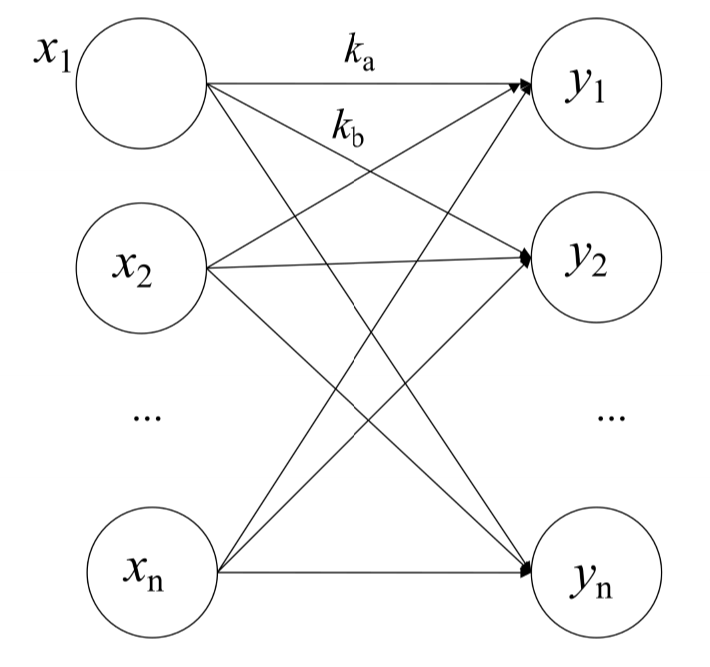
\includegraphics[scale = 0.65]{img/perfect1.png}
        \label{perfect1}
        \caption{Completely bipartite graph}
\end{figure}

\underline{Exercise}: prove that shift cipher with $p_{\cal K}(k) = \frac{1}{|{\cal K}|}=\frac{1}{26}$, i.e., with keys picked at random for each letter of the plaintext, is a perfect cipher. In other words, if we change key any time (not feasible in practice) and we encrypt a letter, then the shift cipher becomes perfect, i.e. unbreakable.

\underline{Solution}: the idea for solving this exercise is to rely on the formal definition we gave above. By using the conditional probability, if we show that $p_{\cal C}(y|x) = p_{\cal C}(y)$ for every $x$ and $y$, then $p_{\cal P}(x|y) = p_{\cal P}(x)$ for every $x$ and $y$, so the cipher is perfect. 

We recall that a shift cipher is defined as:

\begin{itemize}
    \item ${\cal P}={\cal C}={\cal K}=\mathbb{Z}_{26}$;
    \item $E_k(x) = (x+k) \mod 26$;
    \item $D_k(y) = (y-k) \mod 26$.
\end{itemize}

We compute the probability of a generic ciphertext $y$ as:

\begin{array}{rcl} p_{\cal C}(y) &=&\displaystyle \sum_{k \in {\cal K}, \exists x . E_k(x)=y} {p_{\cal K}(k) p_{\cal P}(D_k(y))}\\&=&\displaystyle \frac{1}{26}\sum_{k \in {\cal K}, \exists x . E_k(x)=y} { p_{\cal P}(D_k(y))}\\&=&\displaystyle \frac{1}{26}\sum_{k \in {\cal K}} { p_{\cal P}(y-k \mod 26)}\\&=&\displaystyle \frac{1}{26}\sum_{x \in {\cal P}} { p_{\cal P}(x)}=\frac{1}{26}\end{array}

Notice that:

\begin{itemize}
    \item The first step comes from the fact that each $p_{\cal K}(k)$ is independent of we key we choose, since it is a constant value equal to $\frac{1}{26}$;
    \item The last two steps hold since for each key $k$, we always have a plaintext that gives $y$ when encrypted under $k$. This plaintext is exactly $y-k \mod 26$. So the constraint $\exists x . E_k(x)=y$ always holds and $D_k(y) = y-k \mod 26$;
    \item Then, it is sufficient to observe that $y-k \mod 26$ for all possible keys gives exactly the set of all possible plaintexts ${\cal P}$ and the sum of all their probabilities gives 1.
\end{itemize}

We can now compute

$$p_{\cal C}(y|x) = \displaystyle \sum_{k \in {\cal K}, E_k(x)=y} {p_{\cal K}(k) } = p_{\cal K}(y-x \mod 26) = \frac{1}{26}$$

Here it is enough to observe that, given $x$ and $y$, there exists a unique key that encrypts $x$ as $y$, which is precisely $y-x\mod 26$ (derived from $y = (x+k) \mod 26$). 

Now Bayes theorem gives:

$$p_{\cal P}(x|y) =\displaystyle \frac{p_{\cal P}(x)p_{\cal C}(y|x)}{p_{\cal C}(y)}=\frac{p_{\cal P}(x)\frac{1}{26}}{\frac{1}{26}} = p_{\cal P}(x)$$

which gives the thesis.

We have seen that if we change key any time we encrypt a letter, a cipher as simple as the shift cipher becomes perfect, i.e., unbreakable. We now present two general results that, in fact, show that this strong requirement is indeed necessary and we cannot hope to develop perfect ciphers without it.

\subsubsection{Important theorems}
\textbf{Theorem 1.} Let $p_{\cal C}(y)>0$ for all $y$. A cipher is perfect \textbf{only if} $|{\cal K}| \geq |{\cal P}|$.

The theorem states a \textbf{necessary condition} of a cipher to be perfect: it must be that the number of keys is at least the same as the number of plaintexts. In other words:

$$
\text{perfect cipher } \xrightarrow{} |\cal K| \geq |\cal P| 
$$

and, conversely,

$$
|K| < |P| \xrightarrow{} \text{ not perfect cipher}
$$

Thus, besides the formal definition, we have a very easy way of proving that the cipher is not perfect

\textbf{Proof}: we first notice that by Bayes theorem we have that a cipher is perfect if an only if $p_{\cal C}(y|x)=p_{\cal C}(y)$ for all $x \in {\cal P}$ and $y \in {\cal C}$. If we fix $x$ we obtain that for each $y$, $p_{\cal C}(y|x)=p_{\cal C}(y)>0$ meaning that there exists at least one key $k$ such that $E_k(x) = y$ (otherwise we would have $p_{\cal C}(y|x)=0$). Notice also that all such keys are different since $E_k$ is a function and we have fixed $x$. In fact, $x$ cannot be mapped to two different ciphertexts by the same key (otherwise $E_k$ would not be a function). Thus we have at least one key for each ciphertext meaning that $|{\cal K}| \geq |{\cal C}|$. Since, for any cipher, $E_k$ injects the set of plaintexts into the set of ciphertext, we also have $|{\cal C}| \geq |{\cal P}|$, which gives the thesis $|{\cal K}| \geq |{\cal P}|$.

\textbf{Theorem 2.} Let $|{\cal P}| = |{\cal C}| = |{\cal K}|$. A cipher is perfect \textbf{if and only if}:

\begin{enumerate}
    \item $p_{\cal K}(k) = \frac{1}{|{\cal K}|} \quad \forall k \in {\cal K}$;
    \item For each $x \in {\cal P}$ and $y \in {\cal C}$ there exists exactly one key $k$ such that $E_k(x)=y$.
\end{enumerate}

Intuitively, the theorem states that for a cipher to be \textbf{perfect} (under the hypothesis that the size of the set of plaintexts, ciphertexts and key is the same) \textbf{keys} should be \textbf{picked at random} for any \textbf{encryption} and each plaintext is mapped into each ciphertext through a unique key.

Conversely, in order to show that a cipher is not perfect, we need to show that either condition (1) or (2) does not hold.

\textbf{Proof}: we prove that a perfect cipher implies the two above conditions. We leave the other side of the implication as an exercise. In Theorem 1 we have seen that, for perfect ciphers, if we fix $x$ we obtain that for each $y$ that $p_{\cal C}(y|x)=p_{\cal C}(y)>0$ meaning that there exists at least one key $k$ such that $E_k(x) = y$ and all of these keys are different. Thus we have $|{\cal K}| \geq |{\cal C}|$. In this theorem we have assumed $|{\cal K}| = |{\cal C}|$, meaning that all of these keys k are unique (otherwise we would have $|{\cal K}| > |{\cal C}|$). Since this holds for each $x$ and $y$ we have proved condition 2. To prove condition 1, it is enough to notice that $p_{\cal C}(y|x)=p_{\cal K}(k)$, i.e., the probability of $y$ given $x$ is equal to the probability of the unique key $k$ that encrypts $x$ into $y$. Thus, $p_{\cal K}(k) = p_{\cal C}(y|x)=p_{\cal C}(y)$ (only one key $k$ maps $x$ into $y$). If we fix $y$ and we consider all possible plaintexts $x$ we obtain all possible keys $k$ and for all of them it holds $p_{\cal K}(k) =p_{\cal C}(y)$, with $p_{\cal C}(y)$ constant. Given that the sum of the probability of all keys must be 1, we obtain $p_{\cal K}(k) = \frac{1}{|{\cal K}|}$ which proves condition 1.

\subsubsection{The one-time-pad}
We conclude giving a famous \textbf{example of a perfect cipher} that has been used in practice. This cipher has been used for the telegraph and is a binary variant of Vigenére with keys picked at random. More precisely we have ${\cal P} = {\cal C}= {\cal K} = \mathbb{Z}_2^d$ (i.e. plaintext, ciphertext and keys can be either 0 or 1, i.e. binary) with $p_{\cal K}(k) = \frac{1}{|{\cal K}|} = \frac{1}{2^d}$ for all $k \in {\cal K}$. Encryption is defined as $E_{(k_1, \ldots, k_d)}(x_1,\ldots,x_d) = (x_1 \oplus k_1, \ldots, x_d \oplus k_d)$ where $\oplus$ is the bitwise XOR operation. We recall that the XOR operation is defined as follows: 

$$
101 \text{ XOR } 011 = 110
$$

We notice that the premise of Theorem 2 holds (set sizes are the same by definition of the cipher). Also condition 1 holds, i.e., $p_{\cal K}(k) = \frac{1}{|{\cal K}|}$ by definition of the cipher. We only need to prove condition 2. Let $x \in {\cal P}$ and $y \in {\cal C}$. We have that the unique key giving $y$ from $x$ is computed as $x \oplus y$, i.e., $(x_1 \oplus y_1, \ldots, x_d \oplus y_d)$. We thus conclude that the cipher is perfect.

Despite being a perfect cipher, we notice how one-time-pad is pretty unfeasible in practice, since it needs to change the key each time.

\subsubsection{Recap}
Shannon theory on perfect ciphers shows that such ideal ciphers exist but require as many keys as the possible plaintexts, and keys need to be picked at random for each encryption. Even if this makes such ciphers unpractical, the one-time-pad has been used for real transmission. The setup consisted of two identical books with thousands of  “random” keys. Each key was used once (from which the name one-time). Once the book had been used completely, new shared books were necessary.

\newpage
\subsection{Exercises}

\begin{enumerate}
    \item Decrypt the following ciphertext using substitution cipher (the language is English):

    \begin{figure}[h!]
        \centering
        
\includegraphics[scale = 0.41]{img/ex1.jpg}
        \label{ex1}
        % \caption{Friedman method: finding the key}
    \end{figure}

    \item Decrypt the following ciphertext using Vigenére cipher (the key is "FLUTE"): STWXXWJ;

    \item Write a program that decrypts the following ciphertext (Vigenére cipher):

    \begin{figure}[h!]
        \centering
        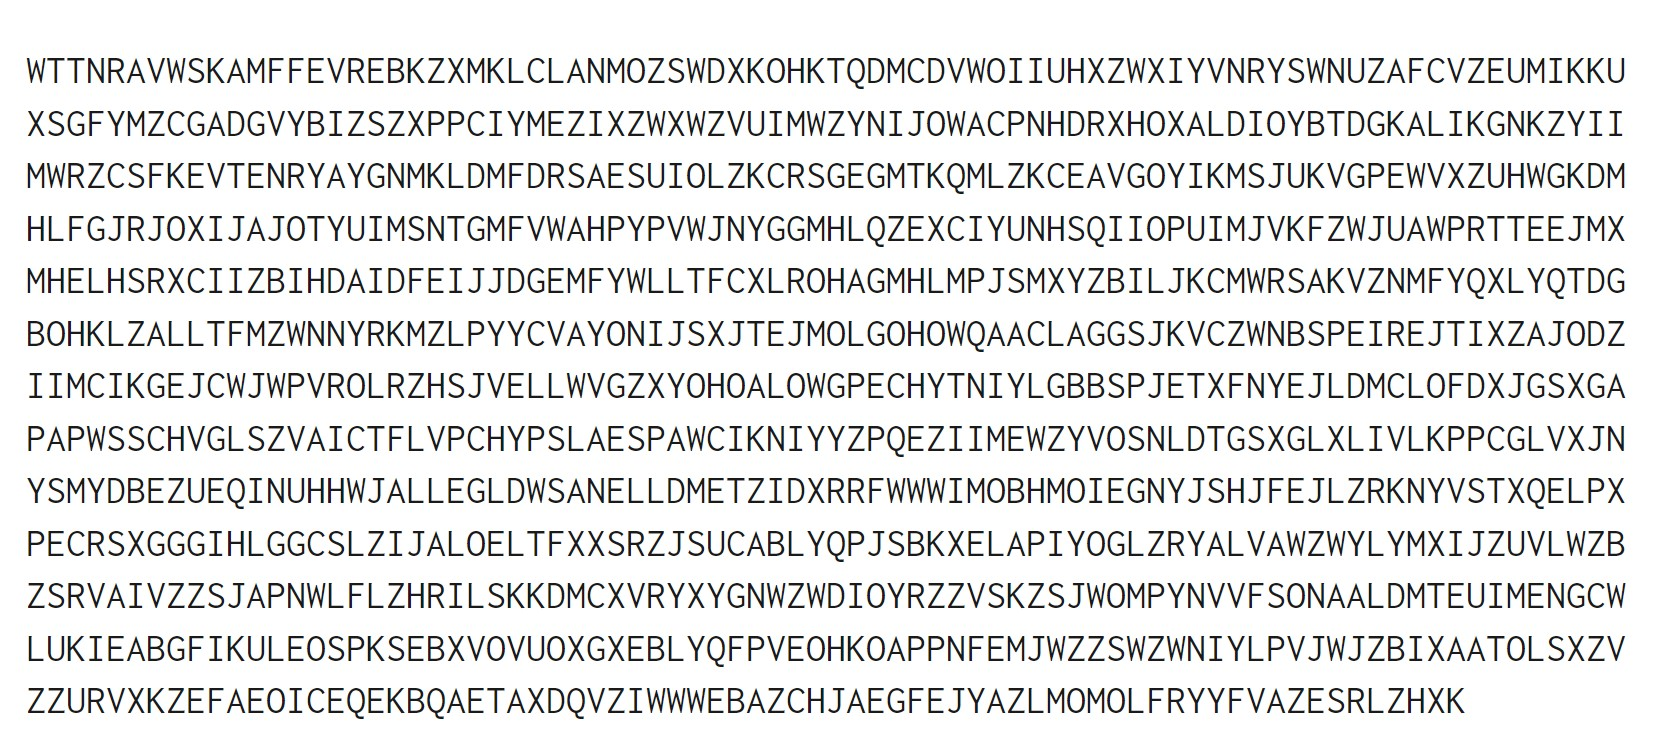
\includegraphics[scale = 0.7]{img/ex3.jpg}
        \label{ex3}
        % \caption{Friedman method: finding the key}
    \end{figure}
    
    \item Encrypt and decrypt message $(2,5)$ using the Hill cipher with $K =  \begin{bmatrix}
5 & 11 \\
8 & 3 
\end{bmatrix};$

    \item Encrypt and decrypt message $(1,3)$ using the Hill cipher with $K = \begin{bmatrix}
1 & 2 \\
4 & 3 
\end{bmatrix}$;

    \item Encrypt and decrypt message $(3,2)$ using the Hill cipher with $K = \begin{bmatrix}
3 & 1 \\
1 & 2 
\end{bmatrix}$

    Solution on slide 2 of L11;

    \item Suppose that we know that FRIDAY has been encrypted as PQCFKU using the Hill cipher, so we have (FRIDAY, PQCFKU). What is the key $K$? Assume $K$ is a 2x2 matrix. Solution on slide 29 of L5;

    \item Compute $\text{gcd}(17,2)$;

    \item Suppose $X = \begin{bmatrix}
5 & 17 \\
8 & 3 
\end{bmatrix}$ and $Y = \begin{bmatrix}
15 & 16 \\
2 & 5 
\end{bmatrix}$. We know that if $X^{-1}$ exists, then $K = X^{-1}Y \mod 26$. Compute $X^{-1}$ using the extended euclidean algorithm and retrieve $K$. Solution on slides 34-35-36 of L5;

    \item Compute $\text{EuclidExt}(14,17)$;

    \item Compute $\text{EuclidExt}(17,5)$. Solution on slide 38 of L5;

    \item Decrypt the following ciphertext, which was encrypted using a \textit{shift cipher}: BEEAKFYDJXUQYHYJIQRYHTYJIQFBQDUJIIKFUHCQD. Solution on slide 27 of L5;

    \item Try to break the following ciphertext encrypted with the autokey cipher: GUAAMLXOOVTMRVTKXOWSSDXNVJSTVTACALTNQFTPNIHUXRPWLV;

    \item Try to extract the plaintext from this word encoded using the autokey cipher. Notice that we do not know the key $k$: FTPNIH. Solution on slide 31-32 of L6;

    \item Prove that the cipher with the following encryption function $E_k(x_1, .., x_d) = (x_1 + k, .., x_d + k) \mod 26$ is not perfect. Use both the formal definition and the theorem 1 discussed in class. Solution on slide 3-4 of L7;

    \item Consider the following cipher with:

    \begin{itemize}
        \item $P = \{a,b\}$;
        \item $K = \{k_1, k_2, k_3\}$;
        \item $C = \{1,2,3,4\}$;
        \item $E_{k_1}(a) = 1$, $E_{k_2}(a) = 2$, $E_{k_3}(a) = 3$, $E_{k_1}(b) = 2$, $E_{k_2}(b) = 3$, $E_{k_3}(c) = 4$
    \end{itemize}

    We now let $p_p(a) = 1/4$, $p_p(b) = 3/4$, $p_{k}(k_1) = 1/2$, $p_{k}(k_2) = p_k(k_3) 1/4$. Compute $p_p(a|1)$, $p_p(a|2)$, $p_p(a|3)$, $p_p(a|4)$, $p_p(b|1)$, $p_p(b|2)$, $p_p(b|3)$, $p_p(b|4)$.
    
\end{enumerate}
\section{Modern cryptography}

\subsection{Composition of ciphers}
So far, we have seen simple historical ciphers and we have discussed how to break them. \textbf{Modern ciphers}, however, are based on very \textbf{simple operations}, such as substitution, XOR, …, that are \textbf{combined} in a smart way so to make the overall algorithm strong and really hard to analyse. It is important to keep in mind that \textbf{combining simple ciphers} does not \textbf{always} \textbf{improve security}. 

For example, consider the shift cipher composed twice. We first shift by $k_1$ and then by $k_2$ modulo 26, as represented in Picture \ref{comp1}.

\begin{figure}[h!]
        \centering
        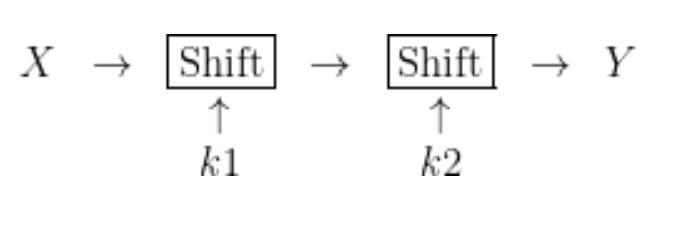
\includegraphics[scale = 1.0]{img/comp1.png}
        \label{comp1}
        \caption{Composition of two shift ciphers - 1}
\end{figure}

It is clear that this is equivalent to shifting by $k_1+k_2$ modulo 26, meaning that applying twice the cipher is the same as applying it once with a key given by the sum of the two keys.

\begin{figure}[h!]
        \centering
        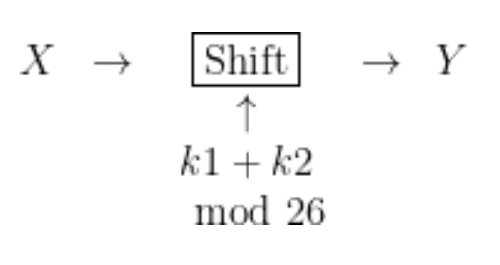
\includegraphics[scale = 1.0]{img/comp2.png}
        \label{comp2}
        \caption{Composition of two shift ciphers - 2}
\end{figure}

This informal reasoning can be made more precise.

\textbf{Definition (Composition)}. We consider two ciphers $S^1=({\cal P}^1,{\cal C}^1,{\cal K}^1,E^1,D^1)$ and $S^2=({\cal P}^2,{\cal C}^2,{\cal K}^2,E^2,D^2)$. We let ${\cal P}^1={\cal C}^1={\cal P}^2={\cal C}^2$, that we note as ${\cal P}$ and ${\cal C}$ in the following. In this way the output of one cipher is for sure a possible plaintext for the second cipher. We can now define \textbf{composition} as $S^1 \times S^2 = ({\cal P},{\cal C},{\cal K}^1\times{\cal K}^2,E,D)$ with

$$
E_{(k1,k2)}(x) = E^2_{k2}(E^1_{k1}(x))
$$

$$
D_{(k1,k2)}(y) = D^1_{k1}(D^2_{k2}(y))
$$

As we can see, in order to encrypt a plaintext $x$ using a composition of two ciphers with keys $k1$ and $k2$ we must:

\begin{enumerate}
    \item \textbf{Encrypt} $x$ using the \textbf{first encryption function} (using $k1$);
    \item \textbf{Encrypt} the \textbf{result} of (1) using the \textbf{second encryption function} (using $k2$).
\end{enumerate}

\underline{Example}: consider the composition of the two shifts above. Formally we have that $E^1_k(x) = E^2_k(x) = x+k \mod 26$. Thus,

\begin{equation}
    \begin{align*}
        E_{(k1,k2)}(x) &= E^2_{k2}(E^1_{k1}(x)) = (x + k1 \mod 26) + k2 \mod 26\\ 
        &= x + (k1+k2 \mod 26) \mod 26 = E^1_{k1+k2 \mod 26}(x)
    \end{align*}
\end{equation}

This proves that composing the shift cipher twice is equivalent to applying it once using as a key the sum of the two keys $k1$ and $k2$, modulo 26.

\subsubsection{Idempotent ciphers}
We have seen that the shift cipher, when repeated twice is equivalent to itself with a different key. When this happens, the cipher $S$ is said to be \textbf{idempotent}, written $S \times S = S$. In this case we know that iterating the cipher will be of no use to improve its security. Even if we repeat it $n$ times we will still get the initial cipher, i.e., $S^n = S$.

We have mentioned that modern ciphers are based on simple operations composed together. Another ingredient is, in fact, \textbf{iteration}. Almost any modern cipher repeats a \textbf{basic core of operations} for a certain number of \textbf{rounds}. It is thus necessary that such core operations do not constitute an idempotent cipher.

It can be proved that if we have two \textbf{idempotent} \textbf{ciphers} that commute, i.e., such that $S^1 \times S^2 = S^2 \times S^1$, then their \textbf{composition} is also \textbf{idempotent}. In this case, we know that iterating their composition is useless. To see why this holds consider one iteration of their composition (recall that function composition is associative):

$$
\begin{array}{ll}(S^1 \times S^2) \times (S^1 \times S^2)\\ = S^1 \times (S^2 \times S^1) \times S^2 &\mbox{ associative property}\\ = S^1 \times (S^1 \times S^2) \times S^2 &\mbox{ commutative property}\\= (S^1 \times S^1) \times (S^2 \times S^2) &\mbox{ associative property}\\ = S^1 \times S^2 &\mbox{ idempotence of the initial ciphers} \end{array}
$$

\subsubsection{Recap}
We have seen examples of how algebraic properties, such as commutativity, can help simplifying the analysis of a cipher. When developing a robust cipher we need to avoid as much as possible that operations can be rearranged, swapped, simplified.

\subsection{The AES cipher}
The \textbf{Advanced Encryption Standard} (AES) has been selected by the National Institute of Standards and Technology (NIST) after a five-year long competition. The original name of the cipher is Rijndael from the names of the two inventors, the cryptographers Joan Daemen and Vincent Rijmen. As any modern cipher, AES is the \textbf{composition} of rather \textbf{simple operations} and contains a \textbf{non-linear component} to \textbf{avoid} \textbf{known-plaintexts attacks} (as the one we have seen on the Hill cipher). The composed operations give a \textbf{non-idempotent cipher} that is \textbf{iterated} for a fixed number of \textbf{rounds} (the longer the key, the more rounds are executed).

Rijndael has been selected because it resulted to be the best one providing:

\begin{itemize}
    \item High \textbf{security} guarantees;
    \item High \textbf{performance};
    \item \textbf{Flexibility} (different key length).
\end{itemize}

All of these \textbf{features} are, in fact, \textbf{crucial} for any modern cipher. Its predecessor, the Data Encryption Standard (DES) is still in use after almost 40 years, in a variant called Triple DES (3DES), which aims at improving the key length. In fact, DES key of only 56 bits is too short to resist brute-forcing on modern, parallel computers.

\subsubsection{Mathematical background}
AES works on the \textbf{Galois Field} with $2^8$ elements noted $\mathbf{GF}(2^8)$. Intuitively, it is the \textbf{set} of all \textbf{8-bit digits} with \textbf{sum} and \textbf{multiplications} performed by interpreting the bits as (binary) \textbf{coefficients of polinomials}. For example, element $11010011$ can be seens as $x^7 + x^6 + x^4 + x + 1$ while $00111010$ is $x^5+x^4+x^3 + x$. The sum will thus be $x^7+x^6+x^4+x+1+x^5+x^4+x^3+x=x^7+x^6+x^5+x^3+1$, since two 1’s coefficient becomes 0, modulo 2, and the term disappears (for example $x + x = 2x = 0x = 0$). We see that \textbf{sum} and \textbf{subtraction} are just the \textbf{bit-wise XOR} of the binary numbers, i.e., $11010011 \oplus 00111010 = 11101001$ which is $x^7+x^6+x^5+x^3+1$.

\textbf{Product} is done \textbf{modulo} the \textbf{irreducible polinomial} $x^8 + x^4 + x^3 + x + 1$. Irreducible means that it cannot be written as the product of two other polinomials (it is, intuitively, the equivalent of primality). 

For example, $(x^7 + x^6 + x^4 + x + 1) \times (x^5+x^4+x^3 + x)$ gives

$$x^{12} + x^{11} + x^9 + x^6 + x^5+x^{11}+x^{10}+x^8+x^5+x^4+x^{10}+x^9+x^7+x^4+x^3+x^8+x^7+x^5+x^2+x$$

, which is reduced to

$$x^{12}+x^6+x^5+x^3+x^2+x$$

Now, the next step is to \textbf{divide} $x^{12}+x^6+x^5+x^3+x^2+x$ by the \textbf{irreducible polynomial} $x^8 + x^4 + x^3 + x + 1$, and find the remainder. In general, long division of polynomials is similar to long division of whole numbers, and when we divide two polynomials we can check the answer using:

$$
\text{dividend} = (\text{quotient} \cdot \text{divisor}) + \text{remainder}
$$

or, equivalently,

$$
\text{dividend} / \text{divisor} = \text{quotient} + \frac{\text{remainder}}{\text{divisor}} 
$$

In our example, dividing $x^{12}+x^6+x^5+x^3+x^2+x$ by $x^8 + x^4 + x^3 + x + 1$ and finding the remainder results as follows:

\begin{enumerate}
    \item Since $x^{12}/x^8 = x^4$, we shift 4 bits to the left the divisor;
    \item Then, we perform a XOR operation between the dividend and the divisor;
    \item Since the results contains 9 bits, which is too much, we perform another XOR operation between the previous result and the divisor;
    \item Finally, we retrieve the remainder, which results to be $11000101$, i.e., $x^7 + x^6 + x^2 + 1$.
\end{enumerate}

$$
\begin{array}{ccccccccccccc}1&0&0&0&0&0&1&1&0&1&1&1&0 \\ 1&0&0&0&1&1&0&1&1 \\\hline & & & &1&1&1&0&1&1&1&1&0\\ & & & &1&0&0&0&1&1&0&1&1 \\\hline & & & & &1&1&0&0&0&1&0&1 \end{array}
$$

This operation is \textbf{quadratic} in general, with respect to the number of bits (8). It can be optimized with the following linear algorithm (which is, in fact, a working python code):

\begin{figure}[h!]
        \centering
        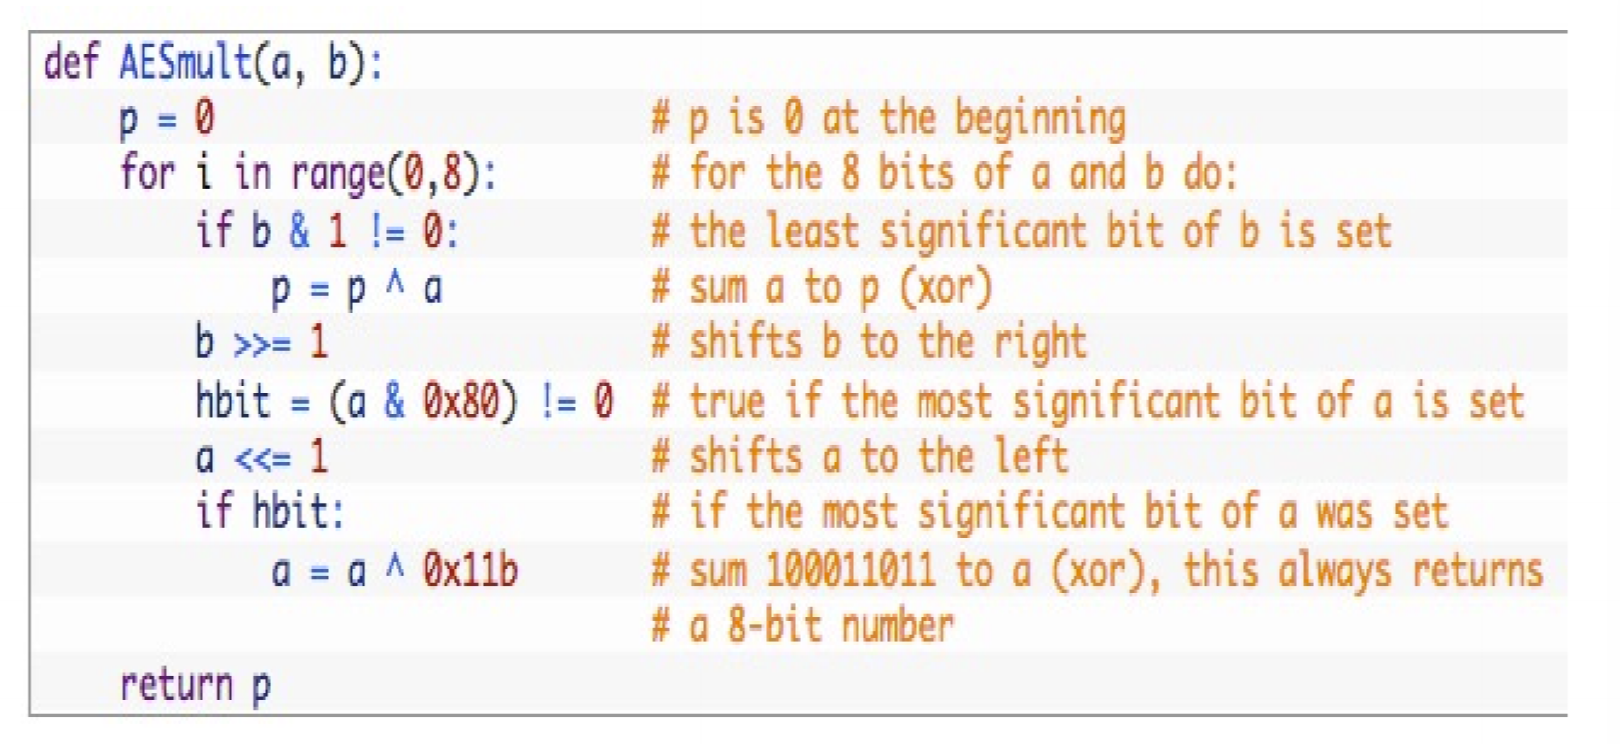
\includegraphics[scale = 0.8]{img/aes1.png}
        \label{aes1}
        \caption{Product - optimization}
\end{figure}

The \textbf{optimization} works as follows:

\begin{enumerate}
    \item We let $a$ to be the binary representation of the coefficients of the first term of the multiplication, and $b$ the binary representation of the coefficients of the second one;
    \item We let $p = 00$;
    \item We perform a XOR operation between $a$ and $p$, and we update $p$ with the result of this operation;
    \item Then, $b$ is shifted to the right and $a$ is shifted to the left meaning that we respectively divide and multiply by $x$ the two polynomials. Now we erase the least significant bit of $b$ and we add a 0 to $a$:
    \begin{itemize}
        \item If the least significant bit was a 1, we continue performing the XOR operation between the new $a$ and $p$;
        \item Otherwise, we skip the XOR operation. 
    \end{itemize}
    \item When $a$ becomes more than $2^8$ we need to XOR to it the modulus $100011011$, i.e. $0x11b$, to keep it 8-bits long.
\end{enumerate}

An example is provided in Picture \ref{aes8}.

\begin{figure}[h!]
        \centering
        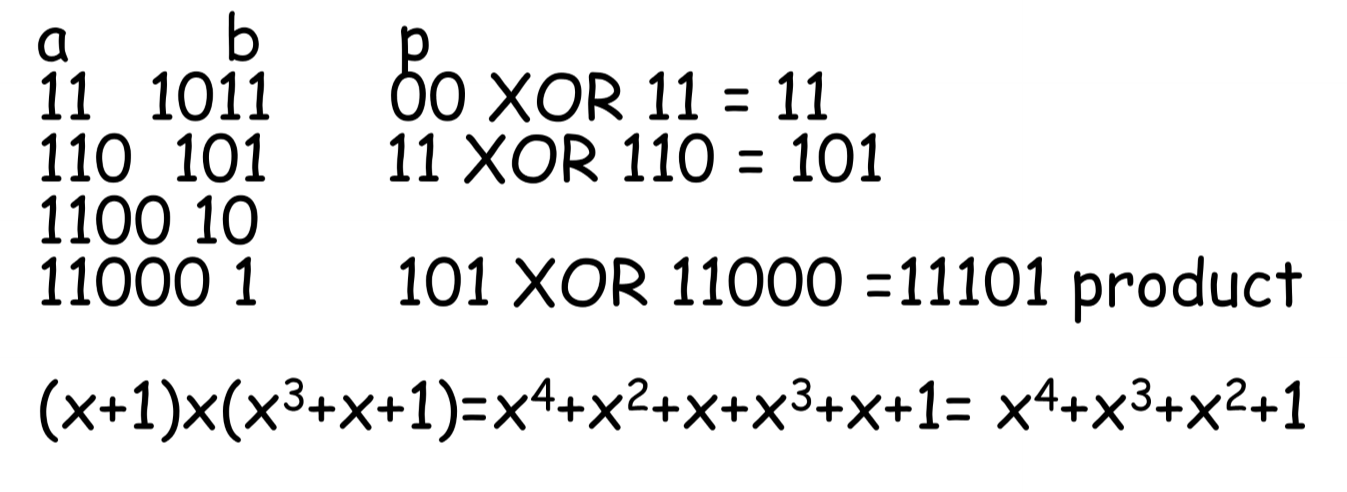
\includegraphics[scale = 0.65]{img/aes8.png}
        \label{aes8}
        \caption{Product - optimization: example}
\end{figure}

The \textbf{correctness} of this algorithm derives from the \textbf{invariant} which states that after each loop: 

\begin{itemize}
    \item $ab+p$ is the product of the initial $a$ and $b$ (all operation does in the Galois Field);
    \item Since $b$ is 0 at the end, we have that $p$ will contain the product.
\end{itemize}

\subsubsection{The AES cipher}
Now that we have introduced the basic operation used to implement AES we can describe the cipher. The official \textbf{description} of \textbf{AES} is available on-line.

AES operates on a \textbf{4×4 matrix} of bytes. We have that 16 bytes are 128 bits which is, in fact, the block size. \textbf{Plaintext} bytes $b_1,\ldots,b_{16}$ are copied in the matrix by columns following this scheme:

$$  \begin{bmatrix}b_1&b_5&b_9&b_{13}\\b_2&b_6&b_{10}&b_{14}\\b_{3}&b_7&b_{11}&b_{15}\\b_4&b_8&b_{12}&b_{16}
    \end{bmatrix}
$$

Cipher \textbf{keys} have lengths of 128, 192, and 256 bits. AES has \textbf{10 rounds} for 128-bit keys, \textbf{12 rounds} for 192-bit keys, and \textbf{14 rounds} for 256-bit keys. Rijndael was designed to handle additional block sizes and key lengths, however they are not adopted in the AES standard. A round is composed of different operations, all of which are invertible:

\begin{enumerate}
    \item \textbf{AddRoundKey}: the round \textbf{key} (see Key Expansion, below) is bitwise \textbf{XOR}-ed with the \textbf{block}. A round key is thus 128 bits, independently of the chosen key size.

    \begin{figure}[h!]
        \centering
        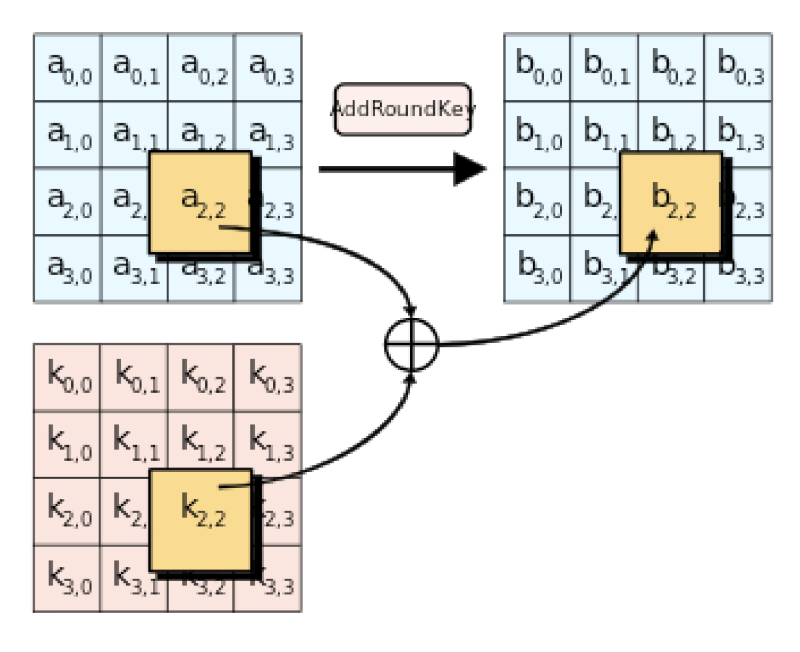
\includegraphics[scale = 0.8]{img/aes2.png}
        \label{aes2}
        \caption{AddRoundKey operation}
    \end{figure}

    In this example, $b_{2,2} = a_{2,2} \text{ XOR } k_{2,2}$.
    
    \item \textbf{SubBytes}: a \textbf{fixed }\textbf{non-linear substitution}, called \textbf{S-box}, is applied to each byte of the block. The substitution is reported below. Given a \textbf{byte} in hexadecimal notation, the \textbf{first digit} is used to select a \textbf{row} and the \textbf{second} one to select a \textbf{column}. For example, $0x25$ would be the third row (2) and the sixth column (5) giving $0x3f$.

    \begin{figure}[h!]
        \centering
        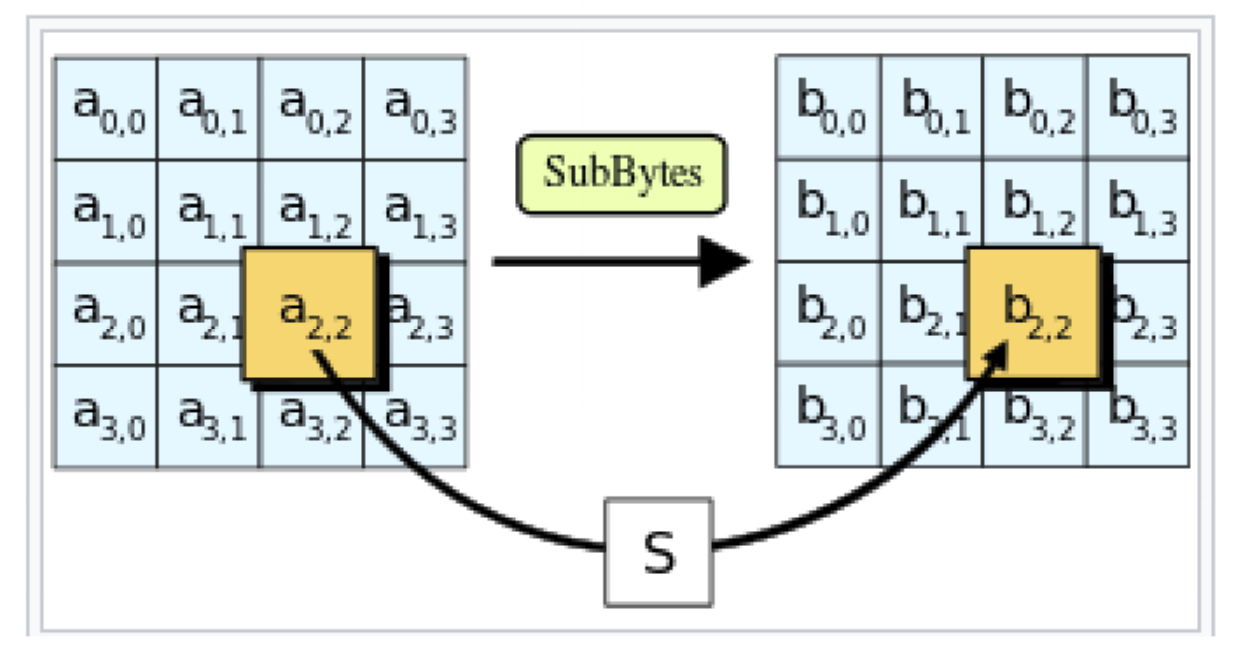
\includegraphics[scale = 0.65]{img/aes3.png}
        \label{aes2}
        \caption{SubBytes operation}
    \end{figure}

    The S-box is represented below:

    \begin{figure}[h!]
        \centering
        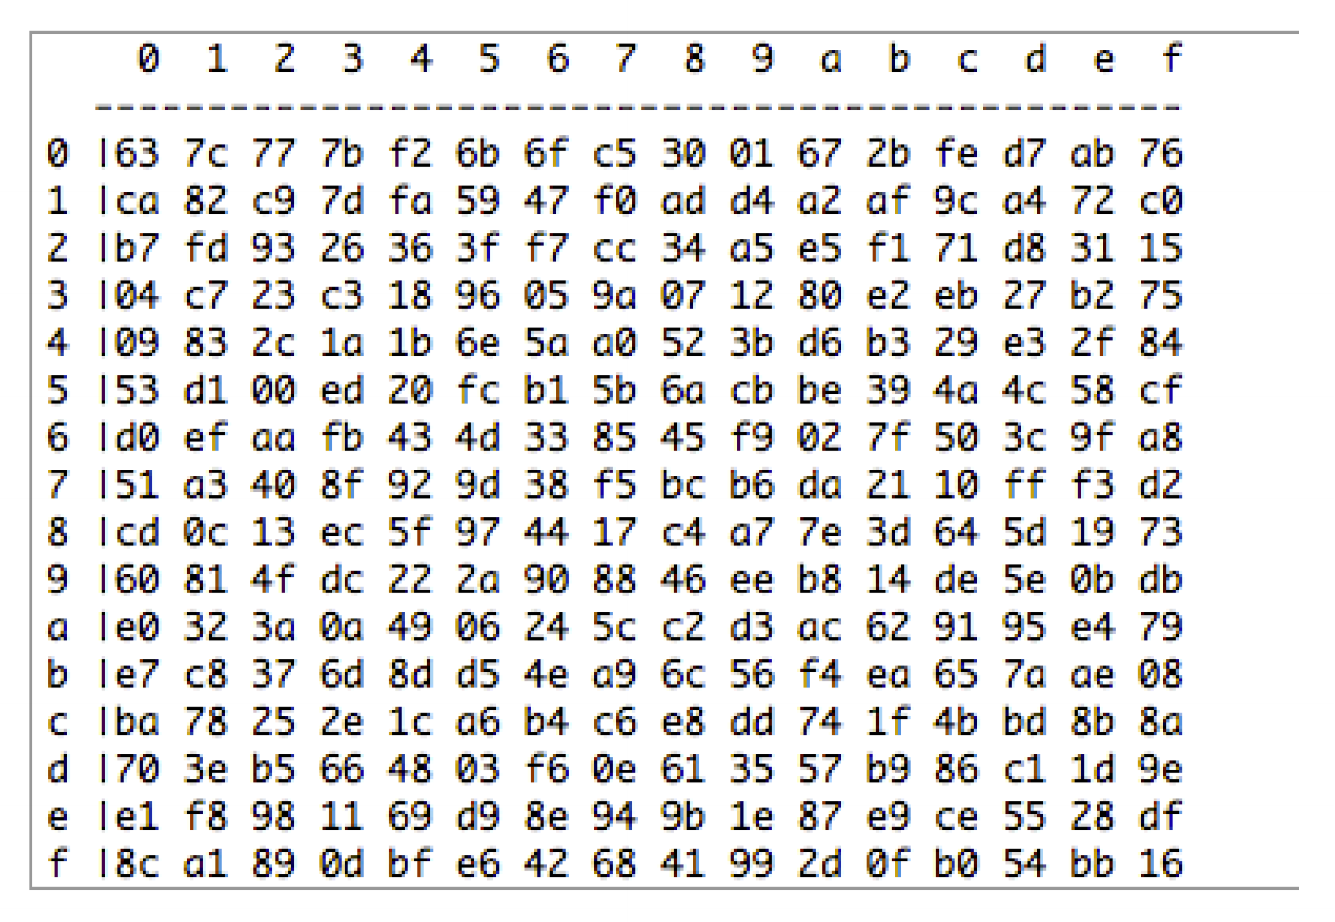
\includegraphics[scale = 0.8]{img/aes4.png}
        \label{aes4}
        \caption{S-box}
    \end{figure}

    Notice that S-box is secure because the attacker cannot easily retrieve $b_{2,2}$, since $2^{16}$ possible values exist. Moreover, this S-box has been obtained by taking, for each byte, its \textbf{multiplicative inverse} in the finite field (that can be computed efficiently via an algorithm that we will see later on), noted $b_7, \ldots, b_0$, and applying the affine transformation $b_i = b_i \oplus b_{i+4 \mod 8} \oplus b_{i+5 \mod 8} \oplus b_{i+6 \mod 8}\oplus b_{i+7 \mod 8} \oplus c_i$, with $c_i$ representing the i-th bit of $01100011$. The above transformation can be written as:

    \begin{figure}[h!]
        \centering
        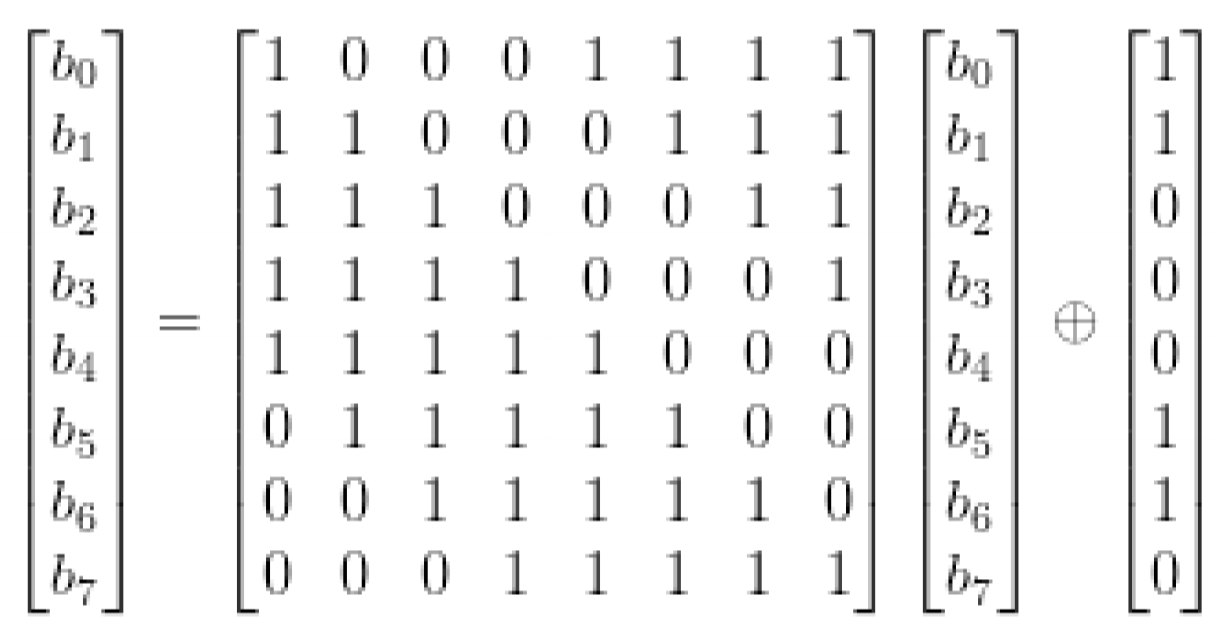
\includegraphics[scale = 0.65]{img/aes5.png}
        \label{aes5}
        \caption{Generation of the S-box}
    \end{figure}

    Using multiplicative inverses is known to give \textbf{non-linear properties}, while the affine transformation complicates the attempt of algebraic reductions.

    \item \textbf{ShiftRows}: \textbf{rows} of the block matrix are \textbf{shifted} to the left by 0,1,2,3, respectively. The shift is circular:

    \begin{figure}[h!]
        \centering
        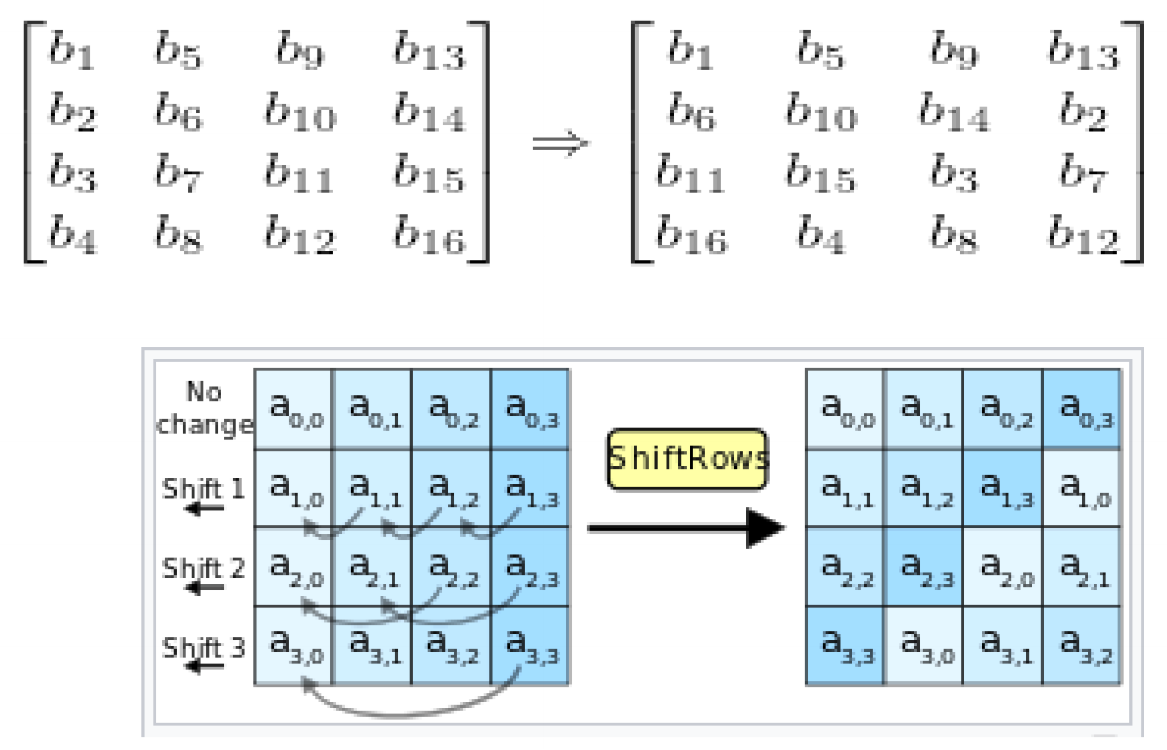
\includegraphics[scale = 0.8]{img/aes6.png}
        \label{aes6}
        \caption{ShiftRows operation}
    \end{figure}

    \item \textbf{MixColumns}: columns of the block matrix are multiplied by the following matrix:

    \begin{figure}[h!]
        \centering
        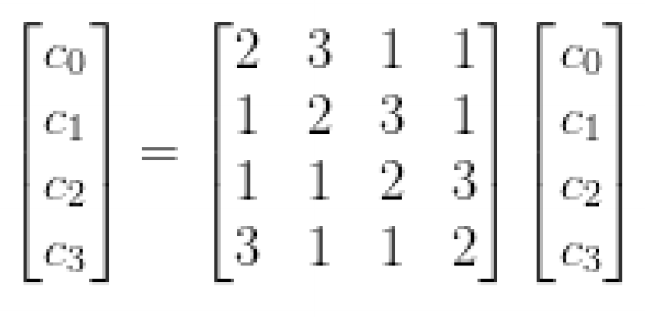
\includegraphics[scale = 0.8]{img/aes7.png}
        \label{aes7}
        \caption{MixColumns operation}
    \end{figure}

    For example the first byte of each column is computed as $2c_0 \oplus 3c_1 \oplus c_2 \oplus c_3$.

    \underline{NOTE}: this fixed matrix is obtained by considering each column as a four-term polynomial with coefficients in $\mathbf{GF}(2^8)$. The columns are then multiplied modulo $x^4 + 1$ with a fixed polynomial $a(x)$, given by $a(x) = 3x^3 + x^2 + x + 2$. This specific modulus is such that, e.g., $x^4$ becomes $x^0$, $x^5$ becomes $x^1$ and so on..

    \item \textbf{Key Expansion} (not covered during the lecture): we have mentioned that AES uses round keys in the AddRoundKey step. These keys are in fact derived from the initial AES key as follows. 
    
    \textbf{Keys} are represented as \textbf{arrays of words} of 4 bytes. So, for example, a 128 bit key will be 4 words of 4 bytes, i.e., 16 bytes. This is expanded into an array of size $4 * (N_r + 1)$, where $N_r$ is the \textbf{number of rounds}. In this way we obtain 4 different words of key for each round.
    
    Let $N_k$ note the \textbf{number of words} of the \textbf{initial key} (e.g. 4 for 128 bits). The first $N_k$ words of the key array are the same as the initial key. Next $i$-th word is obtained from the previous $i-1$ word, possibly transformed as described below, XOR-ed with word $i$-$N_k$. The transformation happens only for words in position multiple of $N_k$ and consists of a cyclic left shift of word bytes by one position (\textit{RotWord}) followed by a byte-wise application of the S-box (\textit{SubWord}) and a XOR with a round constant (\textit{Rcon}). This constant at step $j$ is the word $[x^{j-1},0x00,0x00,0x00]$ with $x^{j-1}$ computed in the Galois field, meaning $02^{j-1}$ since polynomial $x$ is the binary number $00000010$, i.e., $0x02$.

    The pseudocode for this phase is represented Picture \ref{aes9}.

    \begin{figure}[h!]
        \centering
        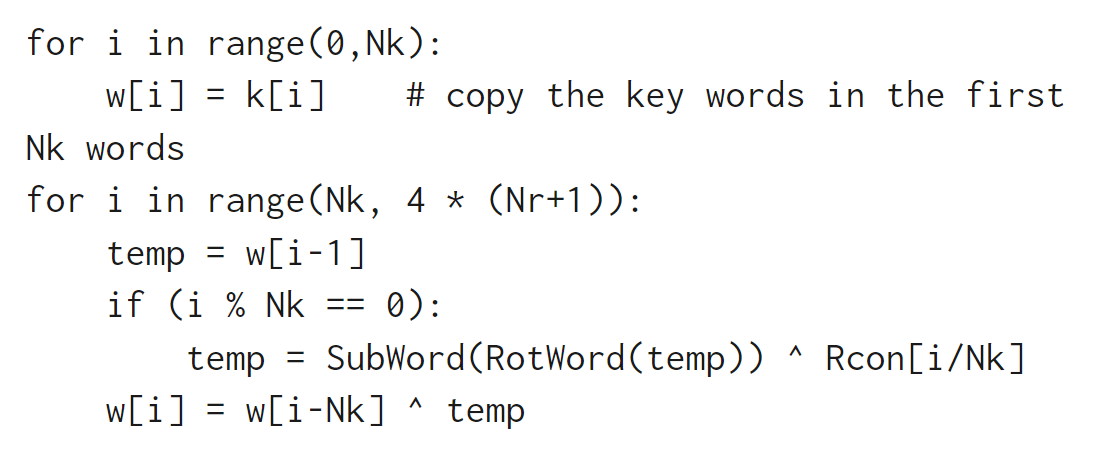
\includegraphics[scale = 0.8]{img/aes9.png}
        \label{aes9}
        \caption{Key Expansion operation}
    \end{figure}

    IMPORTANT NOTE: for 256 bit key, when i-4 is a multiple of $N_k$ \textit{SubWord} is applied to $w[i-1]$ before the XOR. This has been omitted in the code for the sake of readability. Moreover, note that of course the first byte of \textit{Rcon} can be precomputed.

\end{enumerate}

Here is the \textbf{overall scheme} for AES assuming that variable state is initialized with the 4x4 matrix of the plaintext (see above) and $w[]$ has been initialized by key expansion.

\imageLabel{img/aes10.png}{0.8}{Scheme of AES - Encryption}{aes10}

Notice that in the \textbf{last round we do not perform} the \textit{MixColumn} \textbf{operation}.

\textbf{Decryption} is computed by \textbf{applying inverse operations}.

\imageLabel{img/aes11.png}{0.8}{Scheme of AES - Decryption}{aes11}

Notice that:

\begin{enumerate}
    \item \textit{AddRoundKey} is unchanged since XOR is the inverse of itself;
    \item \textit{InvShiftRows} trivially amounts to revert the shifts on the row (to the right instead of left);
    \item \textit{InvSubBytes} is computed by using the following inverse substitution of the S-Box:

    \imageLabel{img/aes12.png}{0.8}{Inverse S-Box}{aes12}

    \item Finally, \textit{InvMixColumns} is given by the following operation:

    \imageB{img/aes13.png}{0.8}

    For example the first byte of each column is computed as $0e c_0 \oplus 0b c_1 \oplus 0d c_2 \oplus 09 c_3$.

    \textbf{NOTE}: this fixed matrix is obtained by considering each column as a four-term polynomial with coefficients in $\mathbf{GF}(2^8)$. The columns are then multiplied modulo $x^4 + 1$ with the inverse of the fixed polynomial $a(x)$, given by $a^{-1}(x) = 0b x^3 + 0d x^2 + 09 x + 0e$.
    
\end{enumerate}

The algorithm for decryption is written in a form similar to the one for encryption but operations are not in the same order. It can, in fact, become the very same algorithm by noticing that:

\begin{enumerate}
    \item \textit{SubBytes} and \textit{ShiftRows} commute. It does not matter if we first apply the byte-wise substitution or if we first shift the rows. The final result will be the same. Of course, the same holds for the inverse transformations;

    \item \textit{InvMixColumns}$(\text{state} \oplus \text{roundKey})$ = \textit{InvMixColumns}(\textit{state}) $\oplus$ \textit{InvMixColumns}(\textit{roundKey}). This allows for inverting the two functions, provided that \textit{InvMixColumns} is applied to the all the round keys.

\end{enumerate}

Call $dw$ the array containing the round keys transformed via InvMixColumns. The final decryption algorithm is represented in Picture \ref{aes16}.

\imageLabel{img/aes16.png}{0.8}{Decryption algorithm}{aes16}

This is exactly the same as the one for encryption, but with the inverse functions. Having the same algorithm for encryption and decryption simplifies a lot implementations, especially if they are done in hardware.

The final scheme of the AES algorithm is provided in Picture \ref{aes14}: note that AES is a symmetric key algorithm.

\imageLabel{img/aes14.png}{0.8}{AES algorithm}{aes14}

Finally, we recall the fact that the security of AES depends on the number of rounds that are executed: the more rounds, the more secure the algorithm is.

\subsection{Block cipher modes of operation}
When using block ciphers we have to face the problem of encrypting \textbf{plaintexts} that are \textbf{longer} than the \textbf{block size}. We then adopt a \textbf{mode of operation}, i.e., a \textbf{scheme} that repeatedly applies the \textbf{block cipher} and allows for encrypting a plaintext of arbitrary size.

\subsubsection{Electronic CodeBlock mode (ECB)}
This is the simplest mode and is, in fact, what we have done so far with classic ciphers: the \textbf{plaintext} $X$ is split into \textbf{blocks} $x_1,x_2,\ldots,x_n$ whose \textbf{size} is exactly the same as the size of the \textbf{cipher block}. Each \textbf{block} is then \textbf{encrypted} independently using the fixed \textbf{key} $k$. For example, a substitution cipher applies to letters. What we do is to split the plaintext into single letters that are encrypted independently.

\image{img/bcm1.png}{0.90}{ECB: Encryption}

\textbf{Decryption} is done, as expected, by reversing the scheme:

\image{img/bcm2.png}{0.90}{ECB: Decryption}

\underline{\textbf{Advantage}}: this scheme has the advantage of being very \textbf{simple} and \textbf{fast}, especially on \textbf{multi-core computers}. Notice, in fact, that each single encryption/decryption can be performed \textbf{independently}.

\underline{\textbf{Disadvantages}}: the \textbf{security} of the scheme, however, is \textbf{poor}. Indeed:

\begin{enumerate}
    \item It mainly conveys all the \textbf{defects} of \textbf{monoalphabetic classic ciphers}: equal plaintext blocks are encrypted in the same way. This allows for the construction of a code-book (from which the mode name) mapping ciphertexts back to plaintexts. It is often the case, in practice, that part of a plaintext is fixed due to the message format, for example. Think of a mail starting with “Dear Alice, …”. If we know a part of the plaintext, we know how the blocks containing that part are encrypted. We can use this information to decrypt other parts of the message, whenever we see the same block occurring.

    Picture \ref{bcm5} provides an immediate visualization of the codebook problem described above.

    \imageLabel{img/bcm5.png}{0.8}{Attack on ECB}{bcm5}

    \item Another crucial limitation of this mode is the complete \textbf{absence of integrity}: an \textbf{attacker} in the middle might duplicate, swap, eliminate encrypted blocks and this would correspond to a plaintext where the same blocks are duplicated, swapped, eliminated. Again, having information about the format of the plaintext, an attacker might be able to obtain a different meaningful plaintext. How critical is this attack really depends on the application. But it is not a good idea to leave such an easy opportunity.
    
\end{enumerate}

\subsubsection{Cipher Block Chaining mode (CBC)}
This mode solves or mitigates all the issues of ECB discussed above: it \textbf{prevents} \textbf{equal plaintexts} to be \textbf{encrypted} the \textbf{same way} and, at the same time, it provides a \textbf{higher degree of integrity}, even if it is not yet satisfactory on this aspect. The idea is to \textbf{“chain” encryption of blocks} using the \textbf{previous encrypted block}. The first block is chained with a special number called \textit{Initialization Vector} (\textit{IV}) that is kept secret together with key $k$.

\image{img/bcm3.png}{0.90}{CBC: Encryption}

\textbf{Decryption} is as follows:

\image{img/bcm4.png}{0.90}{CBC: Decryption}

\underline{\textbf{Advantage}}: as mentioned above, \textbf{CBC} \textbf{never encrypts the same plaintext block in the same way}, preventing the code-book attack. \textbf{Integrity} is improved, but is not yet completely satisfactory. If an attacker swaps, duplicates or eliminates encrypted blocks this will result in at least one corrupted plaintext block. Notice however that this might be unnoticed at the application level and, again, we cannot leave to the application the whole task of checking integrity of decrypted messages.

\underline{\textbf{Disadvantage}}: using \textbf{XOR} introduces a \textbf{new weakness}: the \textbf{attacker} manipulating \textbf{one bit} of an \textbf{encrypted block} $y_i$ obtains that the \textbf{same bit of plaintext} $x_{i+1}$ is also \textbf{manipulated}. At the same time $x_i$ is corrupted.

\subsubsection{Output FeedBack mode (OFB)}
We now see two modes of operation that “transform” block ciphers into stream ciphers. The general idea is to use the block cipher to generate a complex key stream. Encryption is then performed by just XOR-ing the plaintext blocks with the keys of the stream. Intuitively, this is like one-time-pad with a generated key stream. The more the stream is close to a random stream the more the cipher will be close to a perfect one.

\image{img/bcm6.png}{0.90}{OFB: Encryption}

Notice that key generation is completely independent of the plaintext and ciphertext. In fact, it is possible to generate the key stream offline, having key k, and perform encryption later on, when necessary. Decryption simply consists of “swapping the arrows” when performing the XOR: ciphertexts are XOR-ed with the key stream to recover the plaintexts.

\image{img/bcm7.png}{0.90}{OFB: Decryption}

Notice that the generation of the key stream is, in fact, CBC encryption of a zero plaintext (indeed, notice that in this case we do not have the top level $x_i$ XOR $y_{i-1}$). It is thus possible to reuse CBC implementations to compute it. Notice also that the plaintext blocks can be smaller that the size of the block cipher. In that case it is possible to use part of the key and use the remaining part for the next block. For example, if the size of the block is 128 bits (like in AES), and we have to encrypt single bytes we have that one key can be split into $128/8 = 16$ keys of 8 bits, each used to encrypt a single byte.

\underline{\textbf{Advantages}} 

\begin{itemize}
    \item This cipher is very efficient (key can be precomputed using CBC) and allows for the encryption of streams of plaintexts;
    \item Key stream is generated through a block cipher which makes it very hard to be predicted;
    \item Finally, notice that it works very well when IV changes every time we encrypt a new block.
\end{itemize}

\underline{\textbf{Disdvantages}} 

\begin{itemize}
    \item This stream cipher is synchronous since the key stream is independent of the plaintext. As a consequence, if we reuse the same IV with the same key we obtain the same key stream. Since encryption is XOR, attacking the cipher is the same as attacking one-time-pad when the key is used more than once. Thus, the IV must be changed any time we encrypt a new message under the same key k;
    \item Moreover, an attacker in the middle can arbitrarily manipulate bits of the plaintext by swapping the corresponding bits in the ciphertext. No decrypted blocks will be corrupted. For this reason this mode should only be used in application where integrity of the exchanged message is not an issue or is achieved via additional mechanisms. An example could be satellite transmissions where an attacker is extremely unlikely to be in the middle and confidentiality is the only issue. In this setting, absence of integrity becomes useful to avoid noise propagation: an error on one bit will only affect one bit of the plaintext.
\end{itemize}

\underline{NOTE}: there exists a variation of OFB, called \textbf{Counter mode} (\textbf{CTR}), where IV is a random number (nounce) and a counter. The random number can be sent in clear (the bit should change and any new stream generation), and the counter changes the value during the stream generation. This mode is widely used in practice.

\image{img/bcm10.png}{1.8}{CTR: Encryption}

\subsubsection{Cipher FeedBack mode (CFB)}
This mode mitigates the problems of OFB by making the key stream dependent on the previous encrypted element. To preserve the ability of encrypting plaintexts of size less than or equal to the size of the block of the cipher (e.g. a single byte), this mode uses a shift register that is updated at each step: the register is shifted to the left the number of bits of previous ciphertext (8 for a byte), and such a ciphertext is copied into the rightmost bits of the register.

\image{img/bcm8.png}{0.90}{CFB: Encryption}

In this sense, in the first phase we use IV, and in the following ones we use blocks of the previous outputs ($\text{IV}|y_1$ or $y_{n-2}|y_{n-1}$). Decryption is as follows:

\image{img/bcm9.png}{0.90}{CFB: Decryption}

As for OFB, the key stream is generated and then XOR-ed to the ciphertexts to reconstruct the plaintexts.

\underline{\textbf{Advantage}}: this mode provides a higher degree of integrity with respect to OFB: whenever one bit of one ciphertext is modified, the next BSize/CSize plaintexts are corrupted, where BSize is the size of the block of the cipher (e.g., 128 bites) and CSize is the size of the single ciphertext (e.g., 8 bits). For example, with AES and 8 bits of plaintext/ciphertext sizes, we have $128/8 = 16$ corrupted decryptions. This number corresponds to the number of left shifts necessary for a ciphertext to exit the shift register. 

\underline{\textbf{Disadvantage}}: on the other hand, this cipher is slower than OFB as it requires the previous ciphertext to compute the next, meaning that parallelization is impossible when encrypting. Moreover, for noisy transmissions (e.g., satellite, TV, ..) it has the problem of propagating an error on a single bit over the next BSize/CSize plaintexts, which are completely corrupted.

\subsection{More block ciphers}
There are many other ciphers in use, in addition to AES. We list some here giving a very brief summary of their features.

\subsubsection{Data Encryption Standard (DES)}
This is the predecessor of AES. It has been published in 1975 and derives from Lucifer (IBM). It has been the most used and implemented cipher in the history and it is currently used in many application, especially in the triple version below (this version uses 3 keys of 56 bits, which make it invulnerable to brute force attacks). 

DES major problem is the key-length (only 56 bits) that is considered vulnerable with modern parallel computers. Indeed, notice that this key length ony generates $2^{56}$ possible keys, so it is prone to brute force attacks. There are also some analytical results which demonstrate theoretical weaknesses in the cipher, although they are infeasible to mount in practice.

\paragraph{Operations}

The DES cipher takes a fixed-length string of plaintext bits and transforms it through a series of complicated operations into another ciphertext bit string of the same length. We have that:

\begin{itemize}
    \item The block size is 64 bits;
    \item Key is of 56 bits (8 for error correction)
\end{itemize}

The operations are the following:

\begin{itemize}
    \item 16 identical rounds;
    \item Initial permutation (IP) and final permutation (FP, inverse operation);
    \item Before the main rounds, the block is divided into two 32-bit halves and processed alternately:

    \begin{itemize}
        \item The first half is XOR-ed with the result of F, and the result is given as input to the F of the following round;
        \item The second half is provided as input to the F function, and it is also XOR-ed with the result of the F function of the following round.
    \end{itemize}
\end{itemize}

\image{img/des1.png}{0.90}{DES: operations}

\paragraph{Feistel function}

This function is composed of the following operations:

\begin{enumerate}
    \item E: permutation and expansion (from 32 to 48 bits);
    \item Key-mixing (key schedule), where the 48 bits are XOR-ed with a subkey of 48 bits, extracted from the original key (56 bits) using permutation and circular shifts;
    \item Substitution using S-box, and compression (results 32 bits). In this case, from 8 blocks of 6 bits we retrieve 8 blocks of 4 bits;
    \item P: permutation.
\end{enumerate}

\image{img/des2.png}{0.60}{F function}

The result of the F function is a 32-bit information, which is consistent with the previous schema, since it is XOR-ed with half of the original block of 64 bits. The alternation of substitution from the S-boxes, and permutation of bits from the P-box and E-expansion provides so-called "confusion and diffusion” (Shannon).

\paragraph{Confusion and diffusion}

\begin{itemize}
    \item Confusion: the process drastically changes data from the input to the output (e.g., by translating data through a non-linear table created from the key);
    \item Diffusion: changing a single character of the input will change many characters of the output.
\end{itemize}

\subsubsection{International Data Encryption Algorithm (IDEA)}
This cipher was proposed in 1990 as a substitute of DES. It is currently adopted in many applications. 

This cipher is not based on non-linear substitutions (S-Boxes); instead, confusion and diffusion are obtained by a combination of three operations: XOR, sum and multiplication modulo 216. Patent issues have reduced the popularity of this cipher. Compared to other, IDEA performance is not so high.

\subsubsection{Blowfish and Twofish }
Blowfish has been proposed in 1993. It is a cipher with peculiar features: it is very fast, compact and simple to implement, with a very highly configurable security: key length is variable up to 448 bits which allows for security/speed trade-off. As DES it is based on XOR and S-Boxes which are not fixed but computed using the cipher itself and the actual key. These key-dependent S-Boxes make brute-forcing particularly expensive: for each key it is necessary to generate the S-Boxes which takes 522 iterations of the algorithm.

Twofish is one of the finalists of AES and is the “successor” of Blowfish. Both ciphers have been developed by Bruce Schneier.

\subsubsection{RC2, RC5, RC6}
This is a family of ciphers developed by Ron Rivest (one of the fathers for RSA public-key cipher). RC5 (1994) has the peculiar feature of using data dependent rotations. Moreover, the cipher is extremely simple but requires a complex key-expansion procedure: each round is just two XORs, two sums modulo and two rotations. This cipher is highly configurable on the number of rounds, key-length and word-length, which allows for a sophisticate trade-off between security and performance.
RC6 has been one of the AES finalists.

\subsection{Meet-in-the-middle attack - 3DES}
One technique to strengthen ciphers is iteration. We have seen that all modern ciphers are based on rounds, i.e., repetitions of the same core algorithm. We might wonder what happens if we iterate a whole cipher such as DES or AES. There is at least a good reason for that: increasing key length. DES, for example, has a 56-bit key that is considered weak nowadays. If we iterate the cipher using a different key we obtain a key pair (k1,k2) of 112 bits which is, in principle, too hard to break (but we will see that this is not the case).

\subsubsection{3DES}
It is a triple iteration of DES. The aim is to increase the key-length. Due to the meet-in-the-middle attack, the triple key of 168 bits is, in fact, equivalent in strength to a key of 112 bits. Meet-in-the-middle is also the reason why 2DES makes no sense: the 112-bit key could be broken in a 256  time/space complexity brute force attack. 3DES is implemented, for example, in SSH, TLS/SSL and is adopted in many commercial applications. Moreover, bank circuits and credit card issuers use it in smartcard based applications and for PIN protection.

\paragraph{DES is non-idempotent}
We know that iteration makes sense only if the cipher is not idempotent, otherwise the result of its composition would be the same cipher, so it would be useless. The following informal argument suggests that modern ciphers are very unlikely to be idempotent. We reason on DES but the same reasoning would apply to different block ciphers.

DES has a block size of 64 bits. If we list all the $2^{64}$ possible blocks and we pick one DES key, the cipher will map each of these blocks into a different block. Since encryption must be invertible, this mapping is injective. Thus, in any block cipher, a key corresponds to a permutation of all the possible plaintext blocks.

\imageB{img/des3.png}{0.60}

So, for example, 0 (64 zero bits) is mapped to 3214112, 1 to 213210312421 and so on. 

Now, the number of permutations of $2^{64}$ elements is $2^{64}!$ which is enormously big compared to the $2^{56}$ DES keys. We reason as follows: the way a DES key selects a specific permutation is “complex” (otherwise the cipher would be weak). We can thus think of DES keys as selecting a random subset of $2^{56}$ permutations among the $2^{64}!$ possible ones. Now, the probability that the composition of two such permutations is still in this subset is, intuitively, $2^{56} / 2^{64}!$ which is a very small, negligible number. This means that it is really unlikely that 2 iterations of DES (and of any modern block cipher, in fact) correspond to a single encryption under a different key.

As far as DES is concerned, it has been formally proved that it is not idempotent.

\paragraph{Meet-in-the-middle}
We thus consider DoubleDES (2DES), i.e., the iteration of DES twice.

\textit{Is it really true that now, in order to break the cipher, we have to try all the possible key pairs?}

The answer is ‘NO’. We can do better by exploiting the so called Meet-in-the-middle attack. It is a known-plaintext scenario, i.e., the attacker knows pair of plaintext/ciphertext $(X,Y), (X’,Y’), (X'',Y''), ..$ all encrypted under the same key $K$. The idea is:

\begin{enumerate}
    \item Select one pair, say $(X,Y)$, and try to decrypt $Y$ with all the possible second keys $k2$;
    \item All the resulting values $Z$ are stored into a table together with the key, which is indexed by $Z$;
    \item Now we try to encrypt under all the possible first keys $k1$ the plaintext $X$ and we look the obtained value into the table. If we find a match we test the resulting pair $(k1,k2)$ on all the other plaintext/ciphertext pairs and, if all the tests succeeds, we give it as output.
\end{enumerate}

The attack is illustrated below:

\imageB{img/des4.png}{0.50}

The computational cost of this attack is $2^{57}$ steps and $2^{56}$ space. In fact, first step takes $2^{56}$ steps to build a table which is $2^{56}$ entries. Second step takes at most $2^{56}$ steps to find the right key. We thus have $2^{56}$ + $2^{56}$ = $2^{57}$ steps.

\paragraph{False keys}

It is very important that, whenever a pair $(k1,k2)$ for $(X,Y)$ is found, it is tested against other pairs $(X’,Y’)$. It could be the case, in fact, that a key pair is fine for $(X,Y)$ but it is not the right key pair. This can happen more frequently than expected. 

To estimate the number of these false keys we assume that plaintexts are mapped to ciphertext uniformly by the possible keys. In other words, the number of keys mapping $X$ into $Y$ is approximatively the same as the number of keys mapping $X$ into any other ciphertext $Y’$. This assumption typically holds for any good cipher for which observing $Y$ gives very little information about the plaintext $X$. Having a non-uniform distribution would imply that the plaintexts mapped by more keys into $Y$ are more likely than the ones mapped by less keys.

Under this assumption, we can then estimate the number of false keys as $|K|/|C|$, i.e., the number of keys divided by the number of ciphertexts which is, for 2DES, $2^{112}/2^{64} = 2^{48}$. This huge number of possible keys encrypting $X$ into $Y$ can be reduced very quickly by testing keys on more pairs. The probability that a false key is also OK for $(X’,Y’)$ is just 1 over the number of all the possible ciphertexts (we have only one good case $Y’$ over all the possible $2^{64}$ ciphertexts) giving $1⁄2^{64}$ (which is the result of $2^{48} * 1/2^{64}$). Thus, the number of false keys is reduced to $2^{48}⁄2^{64} = 1⁄2^{16}$. If we try on one more pair we get $1⁄2^{80}$, and so on. In summary, with 3 available pairs of plaintext/ciphertext we can run the attack having a negligible probability of getting a false key.

\subsubsection{Recap}
The cost in time is thus basically the same as the one for a single iteration of DES. For this reason, 2DES is never used in practice and, instead, we have a triple iteration known as triple-DES (3DES). This gives a 168-bit triple key $(k1,k2,k3)$. The meet-in-the-middle attack is still possible but it reduces the cost in time to 2112 with a table of size 256 entries. The idea is to build the table by decrypting $Y$ under all $k3$ and then try all the pairs $(k1,k2)$, as illustrated below.

\imageB{img/des5.png}{0.50}

\subsection{Asymmetric-key ciphers}
All the ciphers we have studied so far use the \textbf{same key} $K$ both for \textbf{encryption} and \textbf{decryption}. This implies that the source and the destination of the encrypted data have to \textbf{share} $K$. For this reason, this kind of ciphers are also known as \textbf{symmetric-key ciphers}. This aspect becomes \textbf{problematic} if we want cryptography to \textbf{scale} to big systems with many users willing to communicate securely. Unless we have a centralized service to handle keys (that we will discuss later), for $N$ users this would require $N(N-1)/2$, i.e., $O(N^2)$, keys. For example, for a LAN with 1000 users we would have $\approx 500000$ keys. These keys should be pre-distributed to users in a secure way (e.g., offline). This is totally \textbf{impractical} and would never scale on a wide-area network such as the Internet.

The above argument has been one of the main motivation leading to the \textbf{development} of \textbf{asymmetric-key cryptography}. In \textbf{1976} Diffie and Hellman suggested the existence of this revolutionary ciphers, which are based on the idea that a user $A$ has one \textbf{encrypting} and one \textbf{decrypting} \textbf{key}, which are \textbf{different} but \textbf{correlated} (this is why they are called asymmetric). The characteristic is that the \textbf{encrypting key} is \textbf{public}, while the \textbf{decrypting key} is a \textbf{secret} known only by $A$. In this sense, for $N$ users we have $N$ \textbf{public} keys, which are used for \textbf{encryption}, and $N$ \textbf{private} keys, which are used for \textbf{decryption}. The public key is published in a public list and is known by everybody, even the attacker, and they are correlated with private keys, but the knowledge of the public key does not give any information about the private key.

\subsubsection{Definition}
Intuitively, if we denote with $PK_A$ the public key of $A$ and with $SK_A$ the secret key of $A$, then:

\begin{itemize}
    \item $B$ sends an encrypted message $E_{PK_A}(M)$ to $A$;
    \item $A$ receives it and decrypts it as $D_{SK_A}(E_{PK_A}(M))=M$.
\end{itemize}

Moreover, encryption and decryption algorithms are such that

$$D_{SK_A}(E_{PK_A}(M))=M$$

holds. We can notice that any user can perform the encryption $E_{PK_A}$, so our goal is to define a decryption function that is unfeasible to broke, otherwise the cipher would be useless.

More formally, an asymmetric-key cipher is a \textbf{quintuple} $({\cal P},{\cal C},{\cal K}_S\times{\cal K}_P,E,D)$ with $E : {\cal K}_P \times {\cal P} \rightarrow {\cal C}$ and $D : {\cal K}_S \times {\cal C} \rightarrow {\cal P}$ (\textit{which was the tuple for symmetric ciphers?}) and such that:

\begin{enumerate}
    \item It is \textbf{computationally easy} to generate a \textbf{key-pair} $(SK, PK) \in{\cal K}_S\times{\cal K}_P$;
    \item It is \textbf{computationally easy} to compute $y = E_{PK}(x)$;
    \item It is \textbf{computationally easy} to compute $x = D_{SK}(y)$;
    \item \textbf{Decryption} under $SK$ of a plaintext $x$ \textbf{encrypted} under $PK$ gives the initial \textbf{plaintext} $x$. Formally, $D_{SK}(E_{PK}(x)) = x$;
    \item It is \textbf{computationally infeasible} to compute $SK$ knowing $PK$ and $y$;
    \item It is \textbf{computationally infeasible} to compute $D_{SK}(y)$ knowing $PK$ and $y$ and without knowing $SK$;
\end{enumerate}

Intuitively, instead of one key we now have a \textbf{key pair} $(SK,PK)$ composed of a \textbf{private} and a \textbf{public} key, respectively. \textbf{Encryption} is performed under $PK$ while \textbf{decryption} under $SK$. Thus, \textbf{decryption key} is now \textbf{different} from \textbf{encryption key}. 

Items 1,2 and 3 state that it should be \textbf{practical} to \textbf{generate key pairs} and to encrypt/decrypt data. 

Item 4 states that \textbf{decrypting} under the \textbf{private key} a \textbf{plaintext} \textbf{encrypted} under the \textbf{public key} gives the initial \textbf{plaintext}.

Items 5 and 6 state that the \textbf{cipher} should be \textbf{secure} regardless of the secrecy of the public key $PK$.  This is the \textbf{main challenge} behind this kind of cryptography: the \textbf{public} and the \textbf{private} key have to be \textbf{related}, otherwise decryption would never work, but, at the same time, \textbf{computing} the \textbf{private key} from the public key should be \textbf{impossible} in practice (computationally infeasible).

\subsubsection{Security properties}
What security properties do we have?

\begin{itemize}
    \item \textbf{Secrecy}: this property clearly holds, since we're taking into consideration a cipher;
    \item \textbf{Authentication}: this property does not hold, since the receiver cannot retrieve the identity of the sender, because the key for encryption is public, i.e. known to everybody. Thus, in this case to ensure this property we would also need a digital signature.
\end{itemize}

Notice that in the case of symmetric cipher, both the properties hold, since in that case each sender/receiver share a single key, so the authenticity is ensured.

\subsubsection{One-way trap-door functions}
\textbf{Asymmetric-key ciphers} are strictly \textbf{related} to \textbf{one-way trap-door functions}.

\textbf{Definition.} An \textbf{injective}, \textbf{invertible} \textbf{function} $f$ is \textbf{one-way}, if and only if:

\begin{enumerate}
    \item $y = f(x)$ is \textbf{easy} to compute (i.e. encryption is computationally easy);
    \item $x = f^{-1}(y)$ is \textbf{infeasible} to compute (i.e. decryption is computationally hard).
\end{enumerate}

Note that one-way does not refer to the fact the function does not admit an inverse.: \textbf{one-way} functions are \textbf{invertible} but \textbf{computing their inverse} is too \textbf{expensive} to be feasible in practice.

\textbf{Definition.} An \textbf{injective}, \textbf{invertible} \textbf{family of functions} $f_K$ is \textbf{one-way trap-door}, if and only if, given $K$, we have that:

\begin{enumerate}
    \item $y = f_K(x)$ is \textbf{easy} to compute;
    \item $x = f^{-1}_K(y)$ is \textbf{infeasible} to compute \textbf{without knowing the secret trap-door} $S(K)$ relative to $K$.
\end{enumerate}

Thus, intuitively, the trap-door is a hidden way to go back to the pre-image $x$ of the function: \textbf{only knowing the trap-door we can compute the inverse} of $f_K$.

\subsubsection{The Merkle-Hellman knapsack system}
We present now an example cipher that has been broken, but still gives a very immediate idea of how asymmetric-key ciphers relate to one-way trap-door functions. The cipher is based on the following NP-complete problem.

\paragraph{The subset-sum problem} 
Let $s_1, .., s_n$ and $T$ be positive integers: $s_i$ are \textbf{sizes} while $T$ is the \textbf{target}. A \textbf{solution} to the subset-sum problem is a \textbf{subset} of $(s_1, .., s_n)$ whose \textbf{sum} is exactly the \textbf{target} $T$. 

Formally, the solution is a binary tuple $(x_1, .., x_n)$ such that $\sf\sum_{i=1}^{n}{} x_i s_i = T$.


For example, if sizes are $(4,6,3,8,1)$ and $T=11$, we have that $(0,0,1,1,0)$ and $(1,1,0,0,1)$ are solutions, since $3+8 = 11$ and $4+6+1 = 11$.

This \textbf{problem} is \textbf{NP-complete} in general. As a consequence, we can easily obtain a one-way function from it. Notice, in fact, that NP problems have a non-deterministic polynomial solution meaning that checking if a solution is correct can be done in polynomial time. If we define $f(x_1, .., x_n) = \sf\sum_{i=1}^{n}{} x_i s_i$, we have that $f$ is clearly easy to compute but \textbf{inverting} this function amounts to \textbf{finding} $(x_1, .., x_n)$ from a \textbf{target} $T$ which we know to be \textbf{infeasible} for a big $n$.

How can we now introduce a secret trap-door to allow us inverting the function? The trick is to start from a specific instance of the problem that is easy to solve. We consider special \textbf{sizes} that are \textbf{super-increasing}, i.e., such that $\sf s_i > \sum_{j=1}^{i-1} s_j$, for each $i>1$. Intuitively, any $s_i$ is bigger than the sum of all the previous $s_j$. For example (1,3,5,10) is super-increasing while (1,3,5,9) is not. In this special case there is a very \textbf{efficient algorithm} to solve the \textbf{subset-sum problem}. The idea is to \textbf{start} from the \textbf{biggest element} $s_n$ and go back to the first one: if $s_i$ fits into $T$ we pick it (we set $x_i=1$) and we subtract $s_i$ from $T$. Python example code follows.

\image{img/asy1}{0.5}{Solution of the subset-sum problem with super-increasing sizes}

\underline{Example}: subsetSum($[1,3,5,10]$, 11) returns $[1, 0, 0, 1]$, while subsetSum($[1,3,5,10]$, 12) returns the empty list $[]$, since there's no solution in this case.

\paragraph{The cipher}
We now proceed as follows:

\begin{enumerate}
    \item We start from a \textbf{super-increasing} problem $(s_1,\ldots,s_n)$;
    \item We choose a \textbf{prime} $p > \sum_{i=1}^{n}{s_i}$;
    \item We choose a \textbf{random} $a$ such that $1 < a < p$;
    \item We \textbf{transform} the initial super-increasing problem into $(\hat{s_1}, \ldots, \hat{s_n})$, with $\hat{s_i} = a s_i \mod p$. Notice that \textbf{this problem} is \textbf{not super-increasing in general};
\end{enumerate}

The \textbf{trap-door} is composed of the \textbf{initial problem} and values $p$ and $a$, that are kept \textbf{secret}. Intuitively, \textbf{encryption} is done by \textbf{computing the target} for the \textbf{problem} $(\hat{s_1}, \ldots, \hat{s_n})$. Since this is not super-increasing, finding the initial plaintext $x_1, \ldots, x_n$ is \textbf{infeasible} (for a big $n$). However, \textbf{knowing} the \textbf{secret trap-door} we can \textbf{derive} from the \textbf{ciphertext} a \textbf{target} for the initial easy super-increasing problem, and then solve it using the efficient algorithm above. 

More precisely, \textbf{encryption} and \textbf{decryption} are defined as follows:

\begin{itemize}
    \item $E_{PK}(x_1, \ldots, x_n) = \sum_{i=1}^{n}{x_i \hat{s_i}}$;
    \item $D_{SK}(y)$ is the solution of the super-increasing problem $(s_1,\ldots,s_n)$ with target $a^{-1} y \mod p$.
\end{itemize}

Notice that $a^{-1} \mod p$ is guaranteed to \textbf{exist} by the fact $p$ is a \textbf{prime} number. We will prove this in the next lesson. 

The \textbf{correctness} of the above cipher can be proved as follows:

$$\begin{array}{rcl}E_{PK}(x_1, \ldots, x_n) &=& \sum_{i=1}^{n}{x_i \hat{s_i}}\\ & = & \sum_{i=1}^{n}{a x_i  s_i \mod p}\\& = & a\sum_{i=1}^{n}{x_i  s_i \mod p}\end{array}$$


, thus

$$\begin{array}{rcl}a^{-1}E_{PK}(x_1, \ldots, x_n) \mod p &=& a^{-1} a\sum_{i=1}^{n}{x_i  s_i \mod p}\\ &=& \sum_{i=1}^{n}{x_i  s_i \mod p}\\ &=& \sum_{i=1}^{n}{x_i  s_i}\\\end{array}$$

, since we have that $p > \sum_{i = 1}^n s_i$ by construction. 

The previous equations show that the \textbf{transformed target} $a^{-1} y \mod p$ is, in fact, the \textbf{target} for the \textbf{initial}, easy \textbf{problem}.

\underline{Example}: let $(1,2,5,12)$ be a super-increasing problem. We let $p=23$ and $a=6$. We have that $a^{-1} = 4$, since $6 \cdot 4 \mod 23 = 1$. If we compute $s_i \cdot a \mod p$ we obtain $(6,12,7,3)$ which is not super-increasing. Consider now the plaintext $(1,0,0,1)$. We have that $E_{PK}(1,0,0,1) = 6 + 3 = 9$. Now to decrypt we have to compute $a^{-1} \cdot 9 \mod p = 36 \mod 23 = 13$. We finally solve $(1,2,5,12)$ with target 13, which gives the initial plaintext $(1,0,0,1)$.

\subsection{The RSA cipher}
RSA is the most famous \textbf{asymmetric-key cipher}. It is based on a few technical results from number theory that we recall below.

\subsubsection{Background}

\paragraph{The Euler function} The Euler function $\Phi(n)$ returns the number of numbers less than or equal to $n$ that are coprime to $n$. Recall that $i$ and $n$ are coprime iff $gcd(i,n) = 1$, i.e., if the only common divisor is 1. So, for example, we have that $\Phi(3) = 2$ since 1 and 2 are coprime to 3, $\Phi(4) = 2$ since only 1 and 3 are coprime to 4 and so on. We report some values below:

$$\begin{array}{c|c}n & \Phi(n) \\ \hline 1 & 1\\2 & 1\\3 & 2\\4 & 2\\ 5&4\\ 6&2 \\ 7&6 \\ \end{array}$$

We immediately notice that if $n$ is prime then $\Phi(n) = n-1$. In fact, by definition, a prime number $n$ is coprime to all the numbers smaller than $n$. 

There is another situation where $\Phi(n)$ is easy to compute: when $n=p_1 \ldots p_k$ with $p_1 \neq p_2 \neq \ldots \neq p_k$ prime numbers, i.e. multiplication between prime numbers, we have that $\Phi(n) = \Phi(p_1) \ldots \Phi(p_k) = (p_1-1) \ldots (p_k-1)$.

\underline{Example}: consider $15 = 3 \cdot 5$, then $\phi(15) = \phi(3) \cdot \phi(5) = 2 \cdot 4 = 8$. 

We prove this result for $n = pq$ with $p\neq q$ primes (i.e. we want to prove that $\phi(n) = \phi(p) \phi(q) = (p-1)(q-1)$). The numbers less than $n$ that are not coprime to $n$ is exactly the multiples of $p$ and $q$, i.e., $p,2p,\ldots,(q-1)p,q,2q,\ldots,(p-1)q$ that are $(q-1)+(p-1)$. Now we have that $\Phi(n) = pq-1 - (q-1)-(p-1) = pq -q -p +1  = (p-1)(q-1)$.

\underline{Example}: consider $14 = 2 \cdot 7$. Then, $\phi(14) = 13 - 6 - 1 = 6$, where 6 is the number of multiples of 2 up to 14, while 1 is the only multiple of 7 up to 14.

\subsubsection{The cipher}
RSA stands for Rivest-Shamir-Adleman, the authors of the cipher in 1978. 

We let $n = pq$ with $p,q$ big \textbf{prime} numbers (we need a method for generating large prime numbers, we will consider an algorithm): notice that $\phi(n) = (p-1)(q-1)$. We then choose a small $a$, prime with $\phi(n)$ and smaller than $\phi(n)$. 

\underline{Example}: let $n = 3 \cdot 5$, then $\phi(n) = 2 \cdot 4 = 8$. We can choose $a = 7$.

We compute the unique $b$ s.t. $ab \mod \phi(n) = 1$.

\underline{Example}: considering the previous example, we have that $b = 7$, since $7 \cdot 7 \mod 8 = 1$ (not a good example in this case, since $a = b$).

The \textbf{public key} is $(b,n)$ while the \textbf{private key} (secret trapdoor) is $(a,n)$: notice that $a$ is secret, while $b$ and $n$ are known. We let ${\cal P}={\cal C} = \mathbb{Z}_n$. 

\textbf{Encryption} is defined as $$E_{PK}(x) = x^{b} \mod n$$ while \textbf{decryption} is $$D_{SK}(y) = y^{a} \mod n$$

\underline{Example}: let $p = 5$ and $q = 11$, then $n = 5 \cdot 11 = 55$ and $\phi(n) = 4 \cdot 10 = 40$. We choose $a$ coprime to 40 and smaller than 40, in this case $a = 23$. Thus, $SK = (23, 55)$. We compute the unique $b$ s.t. $ab \mod \phi(n) = 1$, in this case $b = 7$ (computed with the extended Euclidean algorithm). Thus, $PK = (7, 55)$. If we consider the encryption of $x = 2$, then

$$
E_{PK}(2) = 2^{7} \mod 55 = 128 \mod 55 = 18
$$

, while the decryption of 18 results to be

$$
D_{SK}(18) = 18^{23} \mod 55 = 2
$$


\subsubsection{Implementation}
As we will discuss, RSA requires a big modulus $n$ of at least 1024 bits. With these sizes, implementation becomes an issue. For example a linear complexity $O(n)$, that is typically considered very good, is prohibitive as it would require at $2^{1024}$ steps. Every operation should in fact be polynomial with respect to the bit-size $k$.

We first observe that basic operations such as \textbf{sum}, \textbf{multiplication} and \textbf{division} can be performed in $O(k), O(k^2), O(k^2)$, respectively, by using simple standard algorithms (the one we use when we compute operations by hand). Reduction modulo $n$ amounts to compute a division which is, again, $O(k^2)$.

\paragraph{Exponentiation}
This operation is used both for \textbf{encryption} and \textbf{decryption}. First notice that we cannot implement exponentiation to the power of $b$ as $b$ multiplications. In fact, public and private exponents can be the same size as $n$. Performing $b$ multiplications would then require $k^2 2^k$ operation, i.e., $O(2^k)$ which is like brute-forcing the secret trapdoor and infeasible for $k \geq 1024$. We thus need to find some smarter, more efficient way to compute this operation.

\newpage
\subsection{Exercises}
\begin{enumerate}
    \item Show that the composition of the shift cipher with the substitution cipher is still a substitution cipher with a different key. Give a constructive way to derive the new key. What happens if substitution is applied before shift? Solution on slide 23-24-25 of L7;
    \item Consider the composition of Vigenére cipher with key ALICE with the shift cipher with key 8. Is the resulting cipher equivalent to a known one? If so, what is the resulting key? Solution on slide 28 of L7;
    \item Show that the composition of Vigenére and the shift cipher is idempotent. Solution on slide 34 of L7;
    \item Multiply $(x^4 + x^3 + 1) \times (x^5 + 1)$. Solution on slide 17 of L8;
    \item Multiply $(x^4 + x^3 + 1) \times (x^5 + 1)$ using the optimized algorithm. Solution on slide 47 of L8;
    \item Multiply $(x^4 + x) \times (x^3 + 1)$ using the optimized algorithm. Solution on slide 39 of L9;
    \item Multiply $(x^5) \times (x^3 + 1)$ using the optimized algorithm. Solution on slide 41 of L9;
    \item Encode the plaintext "Two One Nine Two" with AES, with the key being "Thats my Kung Fu". Solution on slide 21 to 37 of L9;
    \item Write the expressions for CBC encryption and decryption of the $i$-th block and show, formally, that $D^{CBC}_k(E^{CBC}_k(x_i)) = x_i$.
    
    Hint: to avoid defining a special expression for $y_1$, you can let $y_0 = IV$.

    Solution on slide 2 of L10;

    \item Let $(2, 7, 11, 21, 42, 89, 180, 354)$ be a super-increasing sequence, $p=881$ and $a=588$ (secret key). 
    
    \begin{itemize}
        \item Compute the public key $s_i \cdot a \mod p$;
        \item Then compute the encryption and the decryption of letter “a” (look at the ASCII binary encoding of the letter).
    \end{itemize}

    Solution on slide 16-17 of L12;

    \item Generate two distinct prime numbers, $p=11$ and $q=13$. 
    
    Compute possible $PK, SK, EPK(x), DSK(y)$ with $x=2$. Solution on slide 31-32 of L12.

\end{enumerate}

\section{Applied cryptography}
\subsection{Strong authentication based on symmetric-key cryptography}
We have seen that \textbf{passwords} and \textbf{PINs} suffer from \textbf{interception} and \textbf{replay}: an attacker sniffing a password can reuse it arbitrarily to authenticate. This can be improved using \textbf{OTPs}, i.e., passwords that are never reused. But even in this case, if the attacker is in the middle, he can sniff the password in transit and use it to authenticate once.

The problem with passwords and PIN is that we prove their knowledge by exhibiting the secret value. \textbf{Strong authentication} techniques, instead, allow for \textbf{proving} the \textbf{knowledge} of a secret \textbf{without showing it}. This can be achieved by showing a value that depends on the secret but does not allow to compute it.

\subsubsection{Symmetric key authentication protocols}
We discuss \textbf{strong authentication} protocols based on \textbf{symmetric-key cryptography}. The \textbf{secret} shared among the claimant and the verifier is a \textbf{symmetric cryptographic key}. In order to prove the knowledge of the key $K$, and thus her identity, the claimant sends to the verifier a message encrypted under $K$. Since generating an encrypted message without knowing the key is assumed to be infeasible, this proves its knowledge.

The general \textbf{idea} is to have a \textbf{challenge} and a \textbf{response}:

\begin{itemize}
    \item \textbf{Challenge}: the verifier challenges the claimant to send a particular message encrypted under $K$;
    \item \textbf{Response}: the claimant sends the required message.
\end{itemize}

For example, a challenge might be “send me your name encrypted under $K$”. The response from Alice would then be $E_K(A)$. The verifier will decrypt the message and will check that it matches name A. However, even if this does not reveal $K$, if the challenge is always the same an attacker can simple intercept $E_K(A)$ and replay it to authenticate as Alice. We thus have that the \textbf{challenge} should \textbf{never be the same}. A way to achieve this is to add a \textbf{time-variant parameter}.

\paragraph{Sequence numbers}
The challenge becomes “send me your name and your sequence number encrypted under $K$” with response $E_K(A, seq_A)$. We note the protocol as:

$$A \rightarrow B: E_K(A, seq_A)$$

, i.e. "A sending to B the encryption, under the key $K$, of A and $seq_A$.

The sequence number of Alice is initialized to 0, and then increased by 1 every time so that it never repeats. In a sense, we are following the \textbf{same idea} behind \textbf{OTPs}: we \textbf{never} send the \textbf{same response} twice so that it cannot be replayed. The verifier has to store the last sequence number from Alice so that he can decrypt the message and check that both A and the sequence number (increased by 1) match. In this case he accepts Alice identity and increments the sequence number so that it is ready for next authentication.

Sequence numbers have the \textbf{drawback} of requiring the verifier to store the last sequence number of each possible claimant. Moreover it is \textbf{unclear} what to do if for any reason (system or network failure) the \textbf{sequence numbers go out of sync}: restarting from 0 is unacceptable since any old authentication would become reusable by an attacker. An authenticated protocol to resync is necessary but it cannot be based on sequence numbers, of course.

\paragraph{Timestamps}
The challenge is “send me your name and a recent timestamp encrypted under K”. So the protocol is:

$$A \rightarrow B: E_K(A, t_A) $$

, where the timestamp $t_A$ is the time (integer number) at the local clock of Alice when sending the message. The verifier decrypts the message and check that Alice name matches. Then he extracts a local timestamp $t_B$ and verifies that $t_B-t_A < W$ where $W$ is the acceptance-window, i.e., the maximum allowed delay for the received message. For example, if $W$ is 1 minute the timestamp of A have to be at most 1 minute behind the timestamp of B.

In order to \textbf{prevent replays} we should now pick $W$ so that it is \textbf{big enough} to receive honest messages but so small that no replay will ever be accepted. This is very \textbf{hard} in practice since delays on networks can vary a lot. For this reason, $W$ is typically taken \textbf{much bigger} than the \textbf{average delivery time}. To avoid replays, all the received timestamps are buffered so that double-reception of a valid timestamp can be easily checked. Periodically, the expired timestamps (out of $W$) in the buffer are deleted.

For example consider the following message, intercepted by the attacker:

$$A \rightarrow B: E_K(A, t_A)$$ 

Bob accepts Alice identity and stores $t_A$ in the buffer. The attacker $E$ tries a replay still inside $W$ (we write $E(A)$ to note the attacker pretending to be Alice):

$$E(A) \rightarrow B: E_K(A, t_A)$$

The timestamp is still valid but Bob finds it in the buffer and refuses authentication. Later on, when $t_A$ expires it is deleted from the buffer. Any further attempt of replay from the attacker will be refused since $t_A$ is out of $W$.

Timestamps do not require to store any per-user information (such as sequence numbers). It is enough to termporarily buffer the received-and-still-valid timestamps. Moreover, in case synchrony is lost it is enough to synchronize local clocks. It is however important to notice that this \textbf{synchronization} should be \textbf{authenticated} as \textbf{malicious} changes in clocks might easily allow the attacker to make \textbf{old timestamps valid} or to prevent any honest message to be accepted. As for sequence numbers, this authenticated synchronization cannot be implemented based on timestamps.

\paragraph{Nonces}
We have seen that sequence numbers and timestamps are based on some form of authenticated synchronization. We thus need at least one time variant parameter that do not assume any form of synchronization and can be used, if needed, to synchronize sequence numbers and clocks. 

Nonces are “Numbers used only once”, and here the challenge implies an \textbf{additional} \textbf{message} from the \textbf{verifier} to the claimant containing the nonce (notice that in this case we have a 2-steps protocol, while the previous ones were 1-step protocols). The challenge is “send me your name and nonce $N_B$ encrypted under key $K$”.

$$\begin{array}{l} B \rightarrow A: N_B\\A \rightarrow B: E_K(A, N_B) \end{array}$$

Bob generates a random nonce $N_B$ and sends it to Alice. He then decrypts the received message and checks that both A and $N_B$ match. In this case he accepts Alice identity. The nonce is discarded as it is supposed to be used only once.

If nonces are \textbf{big enough} (e.g. 128 bits), picking them at \textbf{random} implies that the \textbf{probability} of \textbf{reusing} the same nonce is \textbf{negligible}. Thus any replay will be prevented since the nonce will mismatch with overwhelming probability. An example follows:
$$\begin{array}{l} B \rightarrow E(A): N'_B\\E(A) \rightarrow B: E_K(A, N_B) \end{array}$$

Bob refuses since $N_B \neq N'_B$.

\paragraph{ISO/IEC 9798-2 protocols}
Protocols from the standard ISO/IEC 9798-2 are exactly as the ones discussed above apart that they enclose the identifier of the verifier B (to prevent reflection) instead of A.

\textbf{One-pass unilateral authentication}, i.e. A wants to authenticate with B

$$A \rightarrow B: E_K(ts_A,B)$$
,where $ts_A$ is a timestamp or a sequence number (then B will check is $ts_B - ts_A < W$).

\textbf{Two-pass unilateral authentication}
$$\begin{array}{l} B \rightarrow A: N_B\\A \rightarrow B: E_K(N_B, B) \end{array}$$

\textbf{Two-pass mutual authentication}: here Alice and Bob authenticate each other.
$$\begin{array}{l} A \rightarrow B: E_K(ts_A,B)\\B \rightarrow A: E_K(ts_B,A) \end{array}$$
where $ts_A$, $ts_B$ are either timestamps or sequence numbers. Notice that this is just the composition of two independent unilateral authentication protocols.

\textbf{Three-pass mutual authentication}
$$\begin{array}{l} B \rightarrow A: N_B\\A \rightarrow B: E_K(N_A,N_B,B)\\ B \rightarrow A: E_K(N_B,N_A)\end{array}$$

This protocol can be understood starting from the composition of two unilateral authentications based on nonces:
$$\begin{array}{l} B \rightarrow A: N_B\\A \rightarrow B: N_A,E_K(N_B,B)\\ B \rightarrow A: E_K(N_A,A)\end{array}$$

Now, including the nonce $N_A$ in the encryption of the second message is harmless and makes the two unilateral authentications tied in a unique mutual authentication session. The same holds for adding $N_B$ in the third message. Moreover, the fact that intended receiver (Bob) is specified in the second message together with challenge $N_A$ (that is now encrypted) makes it possible to remove A from the last message, as it is enough to prevent reflections.

\subsubsection{Attacks on cryptography}
Since challenge-response protocols provide cryptographic material to the attacker it is important to avoid as much as possible scenarios that facilitate cryptanalysis. For example, the protocol:

$$A \rightarrow B: E_K(A, t_A) $$

is likely to provide a \textbf{known-plaintext scenario}, since it is not hard to guess the value of Alice time-stamp, with some approximation. 

More critically, the protocol:

$$\begin{array}{l} B \rightarrow A: N_B\\A \rightarrow B: E_K(A, N_B) \end{array}$$

provides a \textbf{(partial) chosen-plaintext scenario} where the attacker can ask for encryption of any plaintext $A,z$ with arbitrary $z$. In fact it in enough for the attacker to impersonate Bob, noted $E(B)$, and send $z$ as nonce:

$$\begin{array}{l} E(B) \rightarrow A: z\\A \rightarrow E(B): E_K(A, z) \end{array}$$

Alice becomes a sort of “encryption oracle”.

To \textbf{avoid} these \textbf{problems} a typical \textbf{countermeasure} is to \textbf{randomize cryptography}. This can be done in different way. For example, by adding a \textbf{random padding} to the plaintext. At a logical level, we can think of appending a random number $R_A$ that we call “confounder”, as follows:
$$A \rightarrow B: E_K(A, t_A,R_A) $$
and
$$\begin{array}{l} B \rightarrow A: N_B\\A \rightarrow B: E_K(A, N_B, R_A) \end{array}$$
In this way, the known and chosen-plaintext scenario are prevented. When decrypting, the random confounder will be ignored by Bob. We will always assume this form of randomization at the cryptographic level, with no need of making it explicit at the protocol level.

\paragraph{Redundancy}
Consider the following protocol based on sequence numbers (but it also works with timestamps):
$$A \rightarrow B: A,E_K(seq_A) $$
The \textbf{identifier} A is sent in the \textbf{clear} while the \textbf{sequence number} in \textbf{encrypted}. Assume that Bob only checks monotonicity of $seq_A$ (i.e. checks if $seq_A > \text{last sequence}$) so to deal more flexibly with network delays (even if some message is lost the next will be accepted as the sequence number will be bigger than the stored one). In this case, if the attacker sends an arbitrary message:
$$E(A) \rightarrow B: A,z $$
the probability that the decryption of $z$ is a valid number bigger than the stored one is probably very high (especially if we start from small sequence numbers). 

Encrypting arbitrary numbers with no format or message redundancy makes it impossible to check the integrity of the decryption: a random $z$ can always be decrypted in a meaningful arbitrary number. The presence of the identifier mitigates this problem since $z$, once decrypted, should at least match A. If A is $n$ bits long the probability that this happen is $1/2^n$.

As for randomization, there are \textbf{standard techniques} to \textbf{add redundancy}: a simple one is to enclose a \textbf{one-way hash} of the encrypted message, called \textbf{witness}, as in $h(seq_A),E_K(seq_A)$. The hash is a \textbf{proof} that the \textbf{sender} \textbf{knows} the \textbf{content} of the \textbf{message}. When Bob decrypts he checks that the hash of the decrypted message matches the received one. The attacker might send arbitrary $w,z$, but with a hash of 128 bits the probability of passing the test would be $1/2^{128}$, thus negligible. The fact the hash is one-way makes this technique applicable even when it is important to preserve the secrecy of the sent message.

\paragraph{Reflection}
We now discuss another reason why it is \textbf{important} to have the \textbf{identifier} encrypted together with a \textbf{time variant parameter}. Consider the protocol
$$A \rightarrow B: A,E_K(t_A) $$
Suppose that Bob is allowed to run the same protocol to authenticate with Alice using the same shared key $K$:
$$B \rightarrow A: B,E_K(t_B)$$ 
The attacker can pretend to be Bob, written E(B), as follows:
$$\begin{array}{l} A \rightarrow E(B): A,E_K(t_A)\\ E(B) \rightarrow A: B,E_K(t_A) \end{array} $$
The message from Alice trying to authenticate with Bob is sent back (reflection) to Alice in a second session where the attacker pretends to be Bob. If this is fast enough to be in the acceptance window Alice accepts the identity of Bob (who is instead the attacker). Notice that this is not a replay: Alice has never received timestamp $t_A$ before. She has generated but never received it, in fact.

This attack shows that the \textbf{symmetry} of the key is \textbf{dangerous} if there is \textbf{no information in the ciphertext} about who are the intender \textbf{sender} and \textbf{receiver}. As a matter of fact, it is enough to specify A or B, as far as Alice and Bob agree on what they expect to see in the message (even one bit would suffice, to indicate the first in alphabetical order, for example).

\subsubsection{Key exchange}
\textbf{Authentication} is always \textbf{preliminary} to some other task that requires \textbf{identification}. However, it is useless to adopt a strong-authentication protocol and then start an unprotected remote session:

$$\begin{array}{l} A \rightarrow B: E_K(ts_A,B)\\A \rightarrow B: M_A \end{array}$$

The attacker can intercept message $M_A$ and substitute it with a different one. If used in this way, strong-authentication becomes the same as OTPs: the attacker, if in the middle, can impersonate the claimant once.

This can be easily solved by \textbf{exchanging} a \textbf{new (session) key} while \textbf{identifying}. Since strong authentication is based on encrypted responses, one simple technique is to \textbf{enclose} the \textbf{new key} \textbf{inside} the \textbf{ciphertext}. Notice that this is \textbf{not possible} with \textbf{password-based authentication}, unless we use passwords to derive cryptographic keys. We obtain the following.

\paragraph{ISO/IEC 11770-2 protocols}

\textbf{One-pass unilateral key-establishment}
$$A \rightarrow B: E_K(ts_A,B,k_s)$$
,where $ts_A$ is a timestamp or a sequence number (then B will check is $ts_B - ts_A < W$).

\textbf{Two-pass unilateral key-establishment}
$$\begin{array}{l} B \rightarrow A: N_B\\A \rightarrow B: E_K(N_B, B,k_s) \end{array}$$

\textbf{Two-pass mutual key-establishment}, here Alice and Bob authenticate each other.
$$\begin{array}{l} A \rightarrow B: E_K(ts_A,B,k_s^A)\\B \rightarrow A: E_K(ts_B,A,k_s^B) \end{array}$$
,where $ts_A$, $ts_B$ are either timestamps or sequence numbers. The session key is then computed as a function (for example a bitwise XOR) of the two subkeys $k_s = f(k_s^A,k_s^B)$.

\textbf{Three-pass mutual key-establishment}
$$\begin{array}{l} B \rightarrow A: N_B\\A \rightarrow B: E_K(N_A,N_B,B,k_s^A)\\ B \rightarrow A: E_K(N_B,N_A,k_s^B)\end{array}$$

Notice that we have the same protocol, but now we're adding the session keys. As above, the session key is computed as $k_s = f(k_s^A,k_s^B)$.

\subsubsection{Server-based protocols}
The point-to-point protocols we have studied so far assume a \textbf{pre-shared key} $K$ between Alice and Bob. This \textbf{does not scale} if we have many users as we should share different keys for any possible pairs (meaning a squared number of keys with respect to the number of users, and specifically $n(n-1)/2$). Moreover, it is \textbf{unclear} \textbf{how} a \textbf{new user} might \textbf{establish} a \textbf{new key} for each different existing user.

Determining a shared-key for symmetric key cryptography, and securely obtaining the public key for public key cryptography, can be solved using \textbf{trusted intermediary}. For symmetric key cryptography, the trusted intermediary is called a \textbf{Key Distribution Center} (KDC), while for public key cryptography, it is called \textbf{Certification Authority} (CA).

The \textbf{Key Distribution Center} (KDC) is a service for distributing new session keys to any pair of user asking for them. The KDC shares one key with each user U, noted $K_U$, and users do not directly share keys among them. When a new user Alice is added she just needs to register to the KDC and get her key $K_A$.

\paragraph{Communication between A and B}
Suppose that A and B want to communicate using symmetric key cryptography and a trusted KDC. They only know their individual keys, $K_{A-KDC}$ and $K_{B-KDC}$, respectively, for communicating securely with the KDC. One of the most famous key-establishment protocol based on symmetric-key cryptography and on a KDC is the Needham-Schroeder shared-key protocol:

$$\begin{array}{lrcl} 1. & A \rightarrow KDC & : & A,B,N_A\\ 2. & KDC \rightarrow A & : & E_{K_A}(k_s,B,N_A,E_{K_B}(k_s,A)) \\ 3. & A \rightarrow B & : & E_{K_B}(k_s,A) \\4. & B \rightarrow A & : &E_{k_s}(N_B)\\ 5. & A \rightarrow B & : & E_{k_s}(N_B-1)\\\end{array}$$
We describe the protocol in detail:

\begin{enumerate}
    \item Alice sends a request to KDC for communicating with B. The request contains a nonce $N_A$;
    \item KDC sends a message encrypted under Alice’s key containing a new session key $k_s$, the name of Bob and the nonce (which are both checked by Alice), plus a message encrypted for Bob;
    \item Alice forwards the message encrypted for Bob to Bob;
    \item Bob decrypts the message and obtains the pair $(k_s , A)$ representing a new session key $k_s$ to be used with user A. He sends a nonce $N_B$ encrypted under the new session key to check that Alice knows the key (this is called the key confirmation step);
    \item Alice decrypts the nonce sent by Bob, decrements it by 1 and sends it back encrypted. In this way she proves the knowledge of the session key.
\end{enumerate}

To understand what security guarantees are provided by the protocol we reason on the various entities involved:

\begin{itemize}
    \item KDC: it generates two messages encrypted under Alice and Bob keys. In this way the KDC is guaranteed that the new session key will only be accessed by Alice and Bob and each of them will know who is the expected counterpart, since the relative identifiers are encrypted together with the session key. For example, when Alice decrypts her message she knows that the intended party is Bob, since B is included in the encryption;
    \item Alice: she challenges the KDC with a nonce to avoid an attacker in the middle can replay old messages from the KDC. In this way she is guaranteed that the key is a new one and that the KDC is in fact answering her request. The first two messages are similar to the two-pass unilateral key-establishment we already discussed;
    \item Bob: he receives a message (from Alice) encrypted by the KDC. This message does not contain any time-variant parameter so it might be a replay of an old message. To mitigate this, Bob challenges Alice to prove she knows the session key by sending a nonce encrypted under the key. Only knowing $k_s$ it is possible to decrypt the nonce and send back its value, decremented by 1.
\end{itemize}

This approach makes sense in a \textbf{local}, controlled \textbf{environment} (such as computer science department or a private company), but it \textbf{does not scale} to a \textbf{wide area network} such as the Internet, where the entities cannot be all registered under a centralized server.

\subsection{Diffie-Hellman key agreement protocol}
We have seen that sharing secret keys is fundamental for authenticating and running secure sessions. The \textbf{Diffie-Hellman key agreement protocol} allows for ‘magically’ \textbf{establishing} a \textbf{fresh secret key} between Alice and Bob with \textbf{no need of pre-shared keys} or \textbf{secrets} (using an insecure channel). The key can then be used in a symmetric key cipher.

The scheme is based on \textbf{discrete logarithms}. We choose a prime number $p$ and a generator $a$ of $\{1, \ldots ,p-1\}$. A generator $a$ is a number such that $\{ a^1 \mod p, \ldots a^{p-1} \mod p\} = \{ 1, \ldots, p-1 \}$. In other words, if we rise $a$ to all the powers $1, \ldots ,p-1 \mod n$, we obtain all such numbers. In this sense, $a$ can be used to generate the group. 

\example{If $a = 5$ and $p = 23$, we have that $5^1 \mod 23 = 5$, $5^2 \mod 23 = 2$, .., $5^{22} \mod 23 = 1$}

When this happens, we can define the discrete logarithm modulo $p$ of any number $1 \leq b \leq p-1$ as follows: $log_a b$ is the power $i$ such that $a^i \mod p = b$. It is possible to prove that for any prime $p$ there always exists at least one generator $a$ $[1, \text{fact} 2.132]$.

\example{If $b = 2$, then $5^2 \mod 23 = 2$.}

\textbf{Computing} the discrete logarithm modulo $p$ is \textbf{infeasible} for a big prime $p$ such that $p-1$ has at least a big prime factor (this is to prevent the use of the Pohlig–Hellman algorithm which works well only when prime factors of $p-1$ are small). Diffie-Hellman protocol for key agreement picks one of such big primes $p$ and a generator $a$ of $\{1, \ldots, p-1 \}$. The prime $p$ and the generator $a$ are public. Alice and Bob generate two secrets $S_A$, $S_B$ and run the following protocol:

$$\begin{array}{l} A \rightarrow B: a^{S_A} \mod p \\ B \rightarrow A: a^{S_B} \mod p \end{array} $$

Alice and Bob compute the new key respectively as $(a^{S_B})^{S_A} \mod p$ and $(a^{S_A})^{S_B} \mod p$, that clearly give the same value. Computing the secrets $S_A$, $S_B$ from the exchanged messages amounts to compute the discrete logarithm, that we have assumed to be infeasible. Thus, an attacker eavesdropping the exchanged traffic will never be able to compute the new exchanged key.

\image{img/diffie1.png}{0.6}{Diffie-Hellman protocol: scheme}

\example{The prime $p = 23$ and the generator $a = 5$ are public. Alice chooses $S_A = 6$, and Bob chooses $S_B = 15$. What is the new secret key?\\We have $$A \rightarrow B: a^{S_A} \mod p = 5^6 \mod 23 = 8$$ and $$B \rightarrow A: a^{S_B} \mod p = 5^{15} \mod 23 = 19$$ Now, Alice and Bob compute the new key respectively as $$(a^{S_B})^{S_A} \mod p = 19^6 \mod 23 = 2$$ and $$(a^{S_A})^{S_B} \mod p = 8^{15} \mod 23 = 2$$ Alice and Bob now share the secret key $k = 2$.}

\subsubsection{Man-in-the-middle}
Even if Diffie-Hellman protocol has the nice above property about \textbf{key confidentiality}, the fact it is not based on any pre-shared secret makes it completely \textbf{vulnerable} to \textbf{active attackers} that are able to \textbf{intercept} and \textbf{introduce} \textbf{messages} on the network. In particular, an attacker can mount a \textbf{man-in-the-middle attack} where he is able to \textbf{impersonate} Alice with Bob and Bob with Alice. This is easily achieved by establishing two different keys with them, so that he can be in the middle in the subsequent session. The attack works as follows:

$$\begin{array}{cccccl} A  & \rightarrow &  E(B) & & &: a^{S_A} \mod p \\ A & \leftarrow & E(B) & & &: a^{S_E} \mod p \\ & & E(A)  & \rightarrow &  B &: a^{S_E} \mod p \\ & & E(A) & \leftarrow & B &: a^{S_B} \mod p \end{array}$$

Now Alice and Bob respectively share with the attacker keys $k_s^1 = a^{S_AS_E} \mod p$ and $k_s^2 = a^{S_BS_E} \mod p$. Next messages, encrypted under such keys, will all ‘pass through’ the attacker as follows:

$$\begin{array}{cccccl} A  & \rightarrow &  E(B) & & &: E_{k_s^1}(M_A)  \\ & & E(A)  & \rightarrow &  B &: E_{k_s^2}(M_A)   \\ & & E(A) & \leftarrow & B &: E_{k_s^2}(M_B)  \\ A & \leftarrow & E(B) & & &: E_{k_s^1}(M_B)  \end{array}$$

, where we recall that $E(B)$ represents the attacker who pretends to be B.

Alice and Bob believe to communicate in a secure, encrypted way, but the attacker is in fact decrypting and re-encrypting any message they exchange.

\subsubsection{Summary}
\textbf{Diffie-Hellman protocol} is \textbf{secure} only \textbf{against passive attackers}. The absence of any pre-shared secret makes it impossible to authenticate parties. An attacker can easily pretend to be one party and mount man-in-the-middle attacks, as shown above. This protocol can be made secure using digital signatures (so to provide authentication).

\subsection{Strong authentication based on asymmetric-key cryptography}
We have seen that one technique to authenticate and perform session key establishment is to have a \textbf{centralized KDC service} that shares a symmetric key with any registered users. While this solution makes sense in a \textbf{local}, controlled \textbf{environment} (such as a computer science department or a private company), it \textbf{cannot scale} to a wide area network such as the Internet, where entities cannot be all registered under a centralized server.

\textbf{Asymmetric-key protocols} are more \textbf{suitable} in this setting, as they \textbf{allow} for \textbf{authentication} and \textbf{key-establishment} \textbf{without} the \textbf{presence} of \textbf{on-line servers}. We discuss how the previous techniques need to be modified when asymmetric-key cryptography is employed.

\subsubsection{Asymmetric key authentication protocols}
Let us start from a basic, flawed, unilateral authentication protocol based on timestamps inspired to the one we proposed for symmetric-key encryption:
$$A \rightarrow B: E_{PK_B}(A, t_A) $$
Alice sends her name and a valid timestamp to Bob, both encrypted under Bob’s public key $PK_B$. This protocol is far from being correct, since any user can send the very same message to Bob, given that $PK_B$ is public. So, for example, the attacker can easily pretend to be Alice as follows:
$$E \rightarrow B: E_{PK_B}(A, t_E)$$ 
Asymmetric-key encryption never proves the knowledge of a secret as it only requires the knowledge of $PK_B$. Decryption, instead, can be done only when the private key is known. Thus, a correct unilateral authentication protocol can be obtained by challenging Alice to decrypt something. 

The more natural way to achieve this is to adopt a Nonce-based authentication scheme:
$$\begin{array}{l} B\rightarrow A: E_{PK_A}(N_B,B) \\ A\rightarrow B: N_B \end{array}$$
Bob sends a nonce $N_B$ encrypted together with his identifier under the public key of Alice. Only knowing Alice’s private key, it is possible to decrypt the nonce and send back its value in the clear. This proves the knowledge of a secret that only Alice is assumed to possess and provides authentication. The presence of the time-variant nonce prevents possible replays. The reason why it is important to specify the identifier in the first message is to prevent man-in-the-middle attacks. We illustrate this subtle issue on the following mutual-authentication protocol.

The unilateral authentication protocol above can be extended using the Needham-Schroeder public-key protocol (omitted in these notes, for details refere to these notes\footnote{https://secgroup.dais.unive.it/teaching/cryptography/asym-key-authentication/}) in order to provide mutual authentication.

\subsubsection{Signature-based authentication protocols}
Another way to provide \textbf{authentication} and \textbf{key-establishment} using \textbf{asymmetric-key} is combining asymmetric-key \textbf{encryption} and \textbf{digital signatures}. Encryption is needed to protect key confidentiality while signature gives authentication. 

We start from the the basic, flawed unilateral protocol:

$$A \rightarrow B: E_{PK_B}(A, t_A, k_s)$$

However, in this case everybody knows the $PK_B$, so we add a signature from Alice to prove Alice identity: this, in fact, replaces Alice identifier. The timestamp can be sent in the clear. We include Bob’s identifier in the signature since, as we have discussed, it is important to specify the intended receiver of the authenticated exchange. We obtain the following protocol:

$$A \rightarrow B: t_A, E_{PK_B}( k_s,  sign_{A}( B, t_A, k_s )) $$

The problem with this solution is that the message to encrypt will be typically bigger than the size of one block (for RSA, bigger than the modulus since the signature is already, by itself, as big as the modulus). Implementing this protocol would amount to adopt some encryption mode such as CBC, with strong integrity guarantees.

A \textbf{solution} might be to \textbf{separate} \textbf{encryption} and \textbf{signature} as follows:

$$A \rightarrow B: t_A, E_{PK_B}(k_s), sign_{A}( B, t_A, k_s ) $$

A \textbf{symmetric key} is typically much \textbf{smaller} than \textbf{one encryption block} for asymmetric key cryptography (for example, we might have a 1024 bits RSA modulus and a 128 or 256 bits AES symmetric key). The problem with this solution is that signatures sometimes allow for computing the signed message. For example, a “raw” signature implemented as RSA encryption under the private key (with no hash) can be decrypted using the public key, giving the message in the clear and thus the value of the session key. This protocol can be adopted only when the signature scheme prevents the computation of the signed message.

A general solution is thus to \textbf{first encrypt} and then \textbf{sign}.

$$A \rightarrow B: t_A, E_{PK_B}(k_s,A), sign_{A}( B, t_A, E_{PK_B}(k_s,A))$$ 

Since signature can be implemented using hashes we do \textbf{not have length issues} with this protocol. Notice that Alice identifier has been included in the encrypted message since, as usual, we want messages to be explicit about the parties involved in the protocol. More specifically, this \textbf{prevents} that an \textbf{attacker} \textbf{intercepts} the message and signs the (encrypted) key himself. This could be exploited in settings where the protocol gives credit (such as recharging a prepaid card, or getting an award for submitting the solution to a problem). By signing the session key the attacker will get credit for whatever is sent by Alice encrypted under $k_s$. \textbf{Adding} the \textbf{identifier} clearly \textbf{prevents} this \textbf{attack} since Bob will check that the identifier of the signature is the same as the one included in the encrypted message.

\paragraph{Remark} We have seen in numerous examples that when developing an authentication protocols it is important to specify the identifier which is not already implicit in the key. For example if we encrypt under Bob’s public key it is good to specify A. If Alice is signing it is good to include B in the signature.

\paragraph{X.509 strong authentication protocol} If we run the above unilateral authentication protocol twice we basically obtain the X.509 \textbf{strong two-way authentication protocol}:

$$\begin{array}{l} A \rightarrow B: t_A, E_{PK_B}(k^A_s,A), sign_{A}( B, t_A, E_{PK_B}(k^A_s,A)) \\ B \rightarrow A: t_B, E_{PK_A}(k^B_s,B), sign_{B}( A, t_B, E_{PK_A}(k^B_s,B))\end{array} $$

Alice and Bob compute a session key as $k_s = f(k^A_s,k^B_s)$.

\textbf{Mutual authentication} can also be achieved based on nonces as follows:

$$\begin{array}{l} B \rightarrow A: N_B \\ A \rightarrow B: N_A, E_{PK_B}(k^A_s,A), sign_{A}( B, N_A, N_B, E_{PK_B}(k^A_s,A)) \\ B \rightarrow A: E_{PK_A}(k^B_s,B), sign_{B}( A, N_B, N_A, E_{PK_A}(k^B_s,B))\end{array}$$ 

,which is very close to the X.509 strong three-way authentication protocol described here\footnote{https://www.itu.int/rec/T-REC-X.509}.

\subsection{Key management}
We now discuss how keys are managed, stored and checked by parties and KDC servers.

\subsubsection{Symmetric key management}
We have seen that practical authentication protocols based on symmetric keys require the presence of a centralised trusted party that shares one long-term key with each possible user. It is important to have a \textbf{way} to securely \textbf{deal} with these \textbf{keys} so that an attack to the KDC system would not necessarily compromise the keys of all users.

An interesting solution to this problem is provided by \textbf{symmetric key certificates}. The \textbf{trusted party} possesses a \textbf{master key} $K_M$ that it only knows. When a new user $U$ is registered, the respective \textbf{long-term key} $k_U$ is \textbf{generated} and is \textbf{encrypted} under the \textbf{master key} together with the \textbf{identifier} and additional information such as the key lifetime, type, etc. For example, $SCert_U = E_{K_M}(U,k_U,L)$ certifies that user $U$ has key $k_U$ with lifetime $L$.

These \textbf{certificates} can be distributed to users together with their keys and users can freely distribute their certificates to other users, since the encryption under the master key protects the confidentiality of the enclosed keys. The trusted party can completely forget about the keys and ask for certificates when needed. 

\subsubsection{Asymmetric key management}
The idea of certificates is even more important for protocols based on \textbf{asymmetric keys}. In this case, in fact, it is crucial that \textbf{key management} is completely \textbf{decentralised} since we do not want any on-line centralised servers available at each protocol execution.

First notice that the relevant property here is \textbf{authenticity} of \textbf{public keys}. If Alice and Bob want to communicate they need a way to check that public key is the one truly associated with the opposite party. Suppose Alice wants to send Bob a secret message M. It is insecure for Bob to simply send his public key to Alice:

$$\begin{array}{l} B \rightarrow A: PK_B \\ A\rightarrow B: E_{PK_B}(M) \end{array}$$

In fact, an attacker can replace $PK_B$ with his own key:

$$\begin{array}{cccl} E(B) & \rightarrow & A &: PK_E \\ A & \rightarrow & E(B) & : E_{PK_E}(M) \end{array}$$

The attacker can then decrypt the secret message encrypted under his public key.

We need a \textbf{mechanism} that allows Alice to \textbf{check} that the \textbf{received key} is the one belonging to Bob. Public key certificates contains the same informations as the symmetric key ones but, instead of being encrypted under a symmetric master key, they are signed by a Certification Authority (CA), a trusted entity that certifies the authenticity of user’s public keys. For example, $Cert_B = B$, $PK_B$, $L$, $sign_{CA}(B, PK_B, L)$. 

If Alice knows the public key of the CA and Bob sends this certificate, then Alice can check the validity of the key and its association with Bob (B). The protocol becomes:

$$\begin{array}{l} B \rightarrow A: Cert_B \\ A\rightarrow B: E_{PK_B}(M) \end{array}$$

The attacker cannot change the public key as he is not able to forge a signature from the CA.

\paragraph{Certificate chains}
Having just \textbf{root CA’s} signing any certificate in the world \textbf{does not scale} well. It is useful in practice to have different \textbf{levels} of \textbf{certifications} (maybe associated with countries, states, cities, etc.) so that the end user can go the ‘local’ CA. To deal with this \textbf{hierarchical organisation of CA’s} we need to be able to check certificate chains: the root CA certifies the next CA in the hierarchy and so on all the way to the end user. Once we provide the whole \textbf{chain}, it is enough to \textbf{trust} the \textbf{root public key} in order to check all the certificates in the path to the end user.

\image{img/certchain1.png}{0.80}{Certificate chain: example}

Above we illustrate two end users Carol and Dave certified by two different CAs under the same root CA. If Carol wants to communicate with Dave, she needs to send Dave the certificate chain from the root CA to herself: $\mathrm{CA}_1$ certificate signed by $\mathrm{CA}_{root}, \mathrm{CA}_3$ certificate signed by $\mathrm{CA}_1$ and Carol’s certificate signed by $\mathrm{CA}_3$.

\paragraph{Further extensions}
The basic \textbf{hierarchal tree organisation} illustrated above can be extended to multi-trees, where many root CAs are present (as typically happens in browsers): if any users know many root CAs it is enough a chain from one of the roots to a leaf to certify the corresponding user. To avoid storing all the root certificates, root CAs might certify each other so that any root CA is ‘reachable’ by any other.

Interestingly, there are solutions where no centralised authorities are required. In \textbf{Pretty Good Privacy} (PGP) it is proposed a \textbf{web-of-trust}: any \textbf{user} can \textbf{trust} other \textbf{users}. The level of trust might be such that if Alice trusts Bob, any other user certified by Bob is trusted by Alice. In a sense, each user can ‘elect’ other users as CA’s that can be trusted when signing certificates for other users. This can be depicted as a \textbf{general graph} with \textbf{no roots}: a \textbf{path} in the graph represents a \textbf{chain of certificates} from oner user to the other. If we trust the starting user, we can successfully verify the identity and public key of the final user in the path.

\image{img/pgp1.png}{1.0}{PGP: web of trust}

\end{document}
